\documentclass[twoside]{book}

% Packages required by doxygen
\usepackage{calc}
\usepackage{doxygen}
\usepackage{graphicx}
\usepackage[utf8]{inputenc}
\usepackage{makeidx}
\usepackage{multicol}
\usepackage{multirow}
\usepackage{textcomp}
\usepackage[table]{xcolor}

% Font selection
\usepackage[T1]{fontenc}
\usepackage{mathptmx}
\usepackage[scaled=.90]{helvet}
\usepackage{courier}
\usepackage{amssymb}
\usepackage{sectsty}
\renewcommand{\familydefault}{\sfdefault}
\allsectionsfont{%
  \fontseries{bc}\selectfont%
  \color{darkgray}%
}
\renewcommand{\DoxyLabelFont}{%
  \fontseries{bc}\selectfont%
  \color{darkgray}%
}

% Page & text layout
\usepackage{geometry}
\geometry{%
  a4paper,%
  top=2.5cm,%
  bottom=2.5cm,%
  left=2.5cm,%
  right=2.5cm%
}
\tolerance=750
\hfuzz=15pt
\hbadness=750
\setlength{\emergencystretch}{15pt}
\setlength{\parindent}{0cm}
\setlength{\parskip}{0.2cm}
\makeatletter
\renewcommand{\paragraph}{%
  \@startsection{paragraph}{4}{0ex}{-1.0ex}{1.0ex}{%
    \normalfont\normalsize\bfseries\SS@parafont%
  }%
}
\renewcommand{\subparagraph}{%
  \@startsection{subparagraph}{5}{0ex}{-1.0ex}{1.0ex}{%
    \normalfont\normalsize\bfseries\SS@subparafont%
  }%
}
\makeatother

% Headers & footers
\usepackage{fancyhdr}
\pagestyle{fancyplain}
\fancyhead[LE]{\fancyplain{}{\bfseries\thepage}}
\fancyhead[CE]{\fancyplain{}{}}
\fancyhead[RE]{\fancyplain{}{\bfseries\leftmark}}
\fancyhead[LO]{\fancyplain{}{\bfseries\rightmark}}
\fancyhead[CO]{\fancyplain{}{}}
\fancyhead[RO]{\fancyplain{}{\bfseries\thepage}}
\fancyfoot[LE]{\fancyplain{}{}}
\fancyfoot[CE]{\fancyplain{}{}}
\fancyfoot[RE]{\fancyplain{}{\bfseries\scriptsize Generated on Wed Nov 7 2018 15\-:15\-:53 for ohm\-\_\-tsd\-\_\-slam\-\_\-ref by Doxygen }}
\fancyfoot[LO]{\fancyplain{}{\bfseries\scriptsize Generated on Wed Nov 7 2018 15\-:15\-:53 for ohm\-\_\-tsd\-\_\-slam\-\_\-ref by Doxygen }}
\fancyfoot[CO]{\fancyplain{}{}}
\fancyfoot[RO]{\fancyplain{}{}}
\renewcommand{\footrulewidth}{0.4pt}
\renewcommand{\chaptermark}[1]{%
  \markboth{#1}{}%
}
\renewcommand{\sectionmark}[1]{%
  \markright{\thesection\ #1}%
}

% Indices & bibliography
\usepackage{natbib}
\usepackage[titles]{tocloft}
\setcounter{tocdepth}{3}
\setcounter{secnumdepth}{5}
\makeindex

% Hyperlinks (required, but should be loaded last)
\usepackage{ifpdf}
\ifpdf
  \usepackage[pdftex,pagebackref=true]{hyperref}
\else
  \usepackage[ps2pdf,pagebackref=true]{hyperref}
\fi
\hypersetup{%
  colorlinks=true,%
  linkcolor=blue,%
  citecolor=blue,%
  unicode%
}

% Custom commands
\newcommand{\clearemptydoublepage}{%
  \newpage{\pagestyle{empty}\cleardoublepage}%
}


%===== C O N T E N T S =====

\begin{document}

% Titlepage & ToC
\hypersetup{pageanchor=false}
\pagenumbering{roman}
\begin{titlepage}
\vspace*{7cm}
\begin{center}%
{\Large ohm\-\_\-tsd\-\_\-slam\-\_\-ref \\[1ex]\large 0.\-1 }\\
\vspace*{1cm}
{\large Generated by Doxygen 1.8.6}\\
\vspace*{0.5cm}
{\small Wed Nov 7 2018 15:15:53}\\
\end{center}
\end{titlepage}
\clearemptydoublepage
\tableofcontents
\clearemptydoublepage
\pagenumbering{arabic}
\hypersetup{pageanchor=true}

%--- Begin generated contents ---
\chapter{Todo List}
\label{todo}
\hypertarget{todo}{}

\begin{DoxyRefList}
\item[\label{todo__todo000008}%
\hypertarget{todo__todo000008}{}%
Namespace \hyperlink{namespaceohm__tsd__slam__ref}{ohm\-\_\-tsd\-\_\-slam\-\_\-ref} ]ns später ändern  
\item[\label{todo__todo000001}%
\hypertarget{todo__todo000001}{}%
Class \hyperlink{classohm__tsd__slam__ref_1_1OdometryAnalyzer}{ohm\-\_\-tsd\-\_\-slam\-\_\-ref\-:\-:Odometry\-Analyzer} ]add function call in Thread\-Localize if you want to use odometry for rescue purposes  
\item[\label{todo__todo000014}%
\hypertarget{todo__todo000014}{}%
Member \hyperlink{classohm__tsd__slam__ref_1_1SlamNode_abe1e2022599a8ce220de76b142486ea8}{ohm\-\_\-tsd\-\_\-slam\-\_\-ref\-:\-:Slam\-Node\-:\-:\-\_\-localizers} ]was macht das hier? storing \-\_\-grid, \-\_\-thread\-Mapping, x\-Offset and y\-Offset of Thread\-Localize  
\item[\label{todo__todo000015}%
\hypertarget{todo__todo000015}{}%
Member \hyperlink{classohm__tsd__slam__ref_1_1SlamNode_a2941b11fc25f02fad3467297f0260fec}{ohm\-\_\-tsd\-\_\-slam\-\_\-ref\-:\-:Slam\-Node\-:\-:\-\_\-service\-Start\-Stop\-S\-L\-A\-M} ]wofür brauchen wir den service?  
\item[\label{todo__todo000012}%
\hypertarget{todo__todo000012}{}%
Member \hyperlink{classohm__tsd__slam__ref_1_1SlamNode_ad57ec9810293549dc803209a950a776f}{ohm\-\_\-tsd\-\_\-slam\-\_\-ref\-:\-:Slam\-Node\-:\-:\-\_\-x\-Off\-Factor} ]same as \-\_\-x\-Off\-Factor -\/ prüfen, glaub das wird nicht verwendet -- launch file params auch löschen  
\item[\label{todo__todo000013}%
\hypertarget{todo__todo000013}{}%
Member \hyperlink{classohm__tsd__slam__ref_1_1SlamNode_a591fdd2fc92e9fd53112b36f0125cf51}{ohm\-\_\-tsd\-\_\-slam\-\_\-ref\-:\-:Slam\-Node\-:\-:\-\_\-y\-Off\-Factor} ]wofür gibt es die offset factors? im slamnode.\-cpp definier ich ja nochmal launch file params für x\-Offset u y\-Offset -\/ sehe keine Verwendung von \-\_\-y\-Off\-Factor 

prüfen, glaub das wird nicht verwendet -- launch file params auch löschen  
\item[\label{todo__todo000011}%
\hypertarget{todo__todo000011}{}%
Member \hyperlink{classohm__tsd__slam__ref_1_1SlamNode_a5b4ee64a1d3b1ead996762adfc95ad94}{ohm\-\_\-tsd\-\_\-slam\-\_\-ref\-:\-:Slam\-Node\-:\-:call\-Back\-Service\-Start\-Stop\-S\-L\-A\-M} (ohm\-\_\-tsd\-\_\-slam\-\_\-ref\-::\-Start\-Stop\-S\-L\-A\-M\-::\-Request \&req, ohm\-\_\-tsd\-\_\-slam\-\_\-ref\-::\-Start\-Stop\-S\-L\-A\-M\-::\-Response \&res)]nachfragen  
\item[\label{todo__todo000002}%
\hypertarget{todo__todo000002}{}%
Member \hyperlink{classohm__tsd__slam__ref_1_1SlamNode_af35bd7adca13df47579a682ab3bb827d}{ohm\-\_\-tsd\-\_\-slam\-\_\-ref\-:\-:Slam\-Node\-:\-:Slam\-Node} (void)]verwirrend  
\item[\label{todo__todo000003}%
\hypertarget{todo__todo000003}{}%
Member \hyperlink{classohm__tsd__slam__ref_1_1SlamNode_a0dbbdf08b6ac75aba94c882715d7f49e}{ohm\-\_\-tsd\-\_\-slam\-\_\-ref\-:\-:Slam\-Node\-:\-:$\sim$\-Slam\-Node} ()]geht das so mit neuer foreach schleifn? prüfen, wenn Thread\-Localize erstellt ist  
\item[\label{todo__todo000009}%
\hypertarget{todo__todo000009}{}%
Class \hyperlink{structohm__tsd__slam__ref_1_1TaggedSubscriber}{ohm\-\_\-tsd\-\_\-slam\-\_\-ref\-:\-:Tagged\-Subscriber} ]nachfragen  
\item[\label{todo__todo000010}%
\hypertarget{todo__todo000010}{}%
Member \hyperlink{structohm__tsd__slam__ref_1_1TaggedSubscriber_a6d4ad13158333a16725cdc1cdd6ab3c2}{ohm\-\_\-tsd\-\_\-slam\-\_\-ref\-:\-:Tagged\-Subscriber\-:\-:topic} (const std\-::string topic)]was macht bool topic fct?  
\item[\label{todo__todo000019}%
\hypertarget{todo__todo000019}{}%
Member \hyperlink{classohm__tsd__slam__ref_1_1ThreadGrid_a3e1350e3d4943ab408ae9b0935300972}{ohm\-\_\-tsd\-\_\-slam\-\_\-ref\-:\-:Thread\-Grid\-:\-:\-\_\-occ\-Grid\-Content} ]eventuell abändern, veraltet  
\item[\label{todo__todo000018}%
\hypertarget{todo__todo000018}{}%
Member \hyperlink{classohm__tsd__slam__ref_1_1ThreadGrid_ab5153ffea8c253924f5d5f1f05d9aa59}{ohm\-\_\-tsd\-\_\-slam\-\_\-ref\-:\-:Thread\-Grid\-:\-:event\-Loop} (void)]können wir bitttttte die occupied cells berechnung mal durchgehen 

unsigned char$\ast$ color\-Buffer -\/ std\-::vector?  
\item[\label{todo__todo000016}%
\hypertarget{todo__todo000016}{}%
Member \hyperlink{classohm__tsd__slam__ref_1_1ThreadGrid_a23ff222ecd6e64afde2e8c926e40889c}{ohm\-\_\-tsd\-\_\-slam\-\_\-ref\-:\-:Thread\-Grid\-:\-:Thread\-Grid} (obvious\-::\-Tsd\-Grid $\ast$grid, ros\-::\-Node\-Handle $\ast$const nh, const double x\-Offset, const double y\-Offset)]warum prv\-Nh ohne string template $<$$>$  
\item[\label{todo__todo000022}%
\hypertarget{todo__todo000022}{}%
Member \hyperlink{classohm__tsd__slam__ref_1_1ThreadLocalize_a45c7b109a3a9f22e0c60111c58eb0dd3}{ohm\-\_\-tsd\-\_\-slam\-\_\-ref\-:\-:Thread\-Localize\-:\-:\-\_\-assigner} ]wo wird der schmarrn denn verwendet bidde sachamol  
\item[\label{todo__todo000020}%
\hypertarget{todo__todo000020}{}%
Member \hyperlink{classohm__tsd__slam__ref_1_1ThreadLocalize_ad1b612e37ab54ffe1958cac7d5f9c89c}{ohm\-\_\-tsd\-\_\-slam\-\_\-ref\-:\-:Thread\-Localize\-:\-:\-\_\-data\-Mutex} ]either this or flags obsolete  
\item[\label{todo__todo000023}%
\hypertarget{todo__todo000023}{}%
Member \hyperlink{classohm__tsd__slam__ref_1_1ThreadLocalize_a4444f42e17414907a35919adc4904268}{ohm\-\_\-tsd\-\_\-slam\-\_\-ref\-:\-:Thread\-Localize\-:\-:\-\_\-filter\-Reciprocal} ]what is this?  
\item[\label{todo__todo000021}%
\hypertarget{todo__todo000021}{}%
Member \hyperlink{classohm__tsd__slam__ref_1_1ThreadLocalize_a2e9f4af9a78a5c16b1a4966b1e28a27b}{ohm\-\_\-tsd\-\_\-slam\-\_\-ref\-:\-:Thread\-Localize\-:\-:\-\_\-ran\-Eps\-Thresh} ]was ist das?  
\item[\label{todo__todo000007}%
\hypertarget{todo__todo000007}{}%
Member \hyperlink{SlamNode_8h_a502d892a0b86363c94e2f11fb2370346}{T\-H\-R\-E\-A\-D\-\_\-\-T\-E\-R\-M\-\_\-\-M\-S} ]in Thread\-Grid wird im Destruktor thread\-::join() aus boost aufgerufen, um auf Beendigung des Threads zu warten. Slam\-Node erbt aber nicht von Thread\-S\-L\-A\-M, also besitzt es auch kein boost object thread. wäre es denkbar das auch damit zu lösen anstatt diese Zeit hier festzusetzen? 
\end{DoxyRefList}
\chapter{Namespace Index}
\section{Namespace List}
Here is a list of all namespaces with brief descriptions\-:\begin{DoxyCompactList}
\item\contentsline{section}{\hyperlink{namespaceohm__tsd__slam__ref}{ohm\-\_\-tsd\-\_\-slam\-\_\-ref} }{\pageref{namespaceohm__tsd__slam__ref}}{}
\end{DoxyCompactList}

\chapter{Hierarchical Index}
\section{Class Hierarchy}
This inheritance list is sorted roughly, but not completely, alphabetically\-:\begin{DoxyCompactList}
\item \contentsline{section}{ohm\-\_\-tsd\-\_\-slam\-\_\-ref\-:\-:Odometry\-Analyzer}{\pageref{classohm__tsd__slam__ref_1_1OdometryAnalyzer}}{}
\item \contentsline{section}{ohm\-\_\-tsd\-\_\-slam\-\_\-ref\-:\-:Slam\-Node}{\pageref{classohm__tsd__slam__ref_1_1SlamNode}}{}
\item \contentsline{section}{ohm\-\_\-tsd\-\_\-slam\-\_\-ref\-:\-:Tagged\-Subscriber}{\pageref{structohm__tsd__slam__ref_1_1TaggedSubscriber}}{}
\item \contentsline{section}{ohm\-\_\-tsd\-\_\-slam\-\_\-ref\-:\-:Thread\-S\-L\-A\-M}{\pageref{classohm__tsd__slam__ref_1_1ThreadSLAM}}{}
\begin{DoxyCompactList}
\item \contentsline{section}{ohm\-\_\-tsd\-\_\-slam\-\_\-ref\-:\-:Thread\-Grid}{\pageref{classohm__tsd__slam__ref_1_1ThreadGrid}}{}
\item \contentsline{section}{ohm\-\_\-tsd\-\_\-slam\-\_\-ref\-:\-:Thread\-Localize}{\pageref{classohm__tsd__slam__ref_1_1ThreadLocalize}}{}
\item \contentsline{section}{ohm\-\_\-tsd\-\_\-slam\-\_\-ref\-:\-:Thread\-Mapping}{\pageref{classohm__tsd__slam__ref_1_1ThreadMapping}}{}
\end{DoxyCompactList}
\end{DoxyCompactList}

\chapter{Class Index}
\section{Class List}
Here are the classes, structs, unions and interfaces with brief descriptions\-:\begin{DoxyCompactList}
\item\contentsline{section}{\hyperlink{classohm__tsd__slam__ref_1_1SlamNode}{ohm\-\_\-tsd\-\_\-slam\-\_\-ref\-::\-Slam\-Node} \\*Main node management of 2\-D slam, contains sub classes and ros interface }{\pageref{classohm__tsd__slam__ref_1_1SlamNode}}{}
\item\contentsline{section}{\hyperlink{structohm__tsd__slam__ref_1_1TaggedSubscriber}{ohm\-\_\-tsd\-\_\-slam\-\_\-ref\-::\-Tagged\-Subscriber} \\*\hyperlink{structohm__tsd__slam__ref_1_1TaggedSubscriber}{Tagged\-Subscriber} struct creates new datatype of subscribers for ros communication }{\pageref{structohm__tsd__slam__ref_1_1TaggedSubscriber}}{}
\item\contentsline{section}{\hyperlink{classohm__tsd__slam__ref_1_1ThreadGrid}{ohm\-\_\-tsd\-\_\-slam\-\_\-ref\-::\-Thread\-Grid} \\*Class implementing a thread that generates an occupancy grid }{\pageref{classohm__tsd__slam__ref_1_1ThreadGrid}}{}
\item\contentsline{section}{\hyperlink{classohm__tsd__slam__ref_1_1ThreadLocalize}{ohm\-\_\-tsd\-\_\-slam\-\_\-ref\-::\-Thread\-Localize} }{\pageref{classohm__tsd__slam__ref_1_1ThreadLocalize}}{}
\item\contentsline{section}{\hyperlink{classohm__tsd__slam__ref_1_1ThreadMapping}{ohm\-\_\-tsd\-\_\-slam\-\_\-ref\-::\-Thread\-Mapping} \\*Implements a thread updating an obvious\-:Tsd\-Grid }{\pageref{classohm__tsd__slam__ref_1_1ThreadMapping}}{}
\item\contentsline{section}{\hyperlink{classohm__tsd__slam__ref_1_1ThreadSLAM}{ohm\-\_\-tsd\-\_\-slam\-\_\-ref\-::\-Thread\-S\-L\-A\-M} \\*Base class implementing boost thread functionality }{\pageref{classohm__tsd__slam__ref_1_1ThreadSLAM}}{}
\end{DoxyCompactList}

\chapter{File Index}
\section{File List}
Here is a list of all files with brief descriptions\-:\begin{DoxyCompactList}
\item\contentsline{section}{src/\hyperlink{slam__node_8cpp}{slam\-\_\-node.\-cpp} }{\pageref{slam__node_8cpp}}{}
\item\contentsline{section}{src/\hyperlink{SlamNode_8cpp}{Slam\-Node.\-cpp} }{\pageref{SlamNode_8cpp}}{}
\item\contentsline{section}{src/\hyperlink{SlamNode_8h}{Slam\-Node.\-h} }{\pageref{SlamNode_8h}}{}
\item\contentsline{section}{src/\hyperlink{ThreadGrid_8cpp}{Thread\-Grid.\-cpp} }{\pageref{ThreadGrid_8cpp}}{}
\item\contentsline{section}{src/\hyperlink{ThreadGrid_8h}{Thread\-Grid.\-h} }{\pageref{ThreadGrid_8h}}{}
\item\contentsline{section}{src/\hyperlink{ThreadLocalize_8cpp}{Thread\-Localize.\-cpp} }{\pageref{ThreadLocalize_8cpp}}{}
\item\contentsline{section}{src/\hyperlink{ThreadLocalize_8h}{Thread\-Localize.\-h} }{\pageref{ThreadLocalize_8h}}{}
\item\contentsline{section}{src/\hyperlink{ThreadMapping_8cpp}{Thread\-Mapping.\-cpp} }{\pageref{ThreadMapping_8cpp}}{}
\item\contentsline{section}{src/\hyperlink{ThreadMapping_8h}{Thread\-Mapping.\-h} }{\pageref{ThreadMapping_8h}}{}
\item\contentsline{section}{src/\hyperlink{ThreadSLAM_8cpp}{Thread\-S\-L\-A\-M.\-cpp} }{\pageref{ThreadSLAM_8cpp}}{}
\item\contentsline{section}{src/\hyperlink{ThreadSLAM_8h}{Thread\-S\-L\-A\-M.\-h} }{\pageref{ThreadSLAM_8h}}{}
\end{DoxyCompactList}

\chapter{Namespace Documentation}
\hypertarget{namespaceohm__tsd__slam__ref}{\section{ohm\-\_\-tsd\-\_\-slam\-\_\-ref Namespace Reference}
\label{namespaceohm__tsd__slam__ref}\index{ohm\-\_\-tsd\-\_\-slam\-\_\-ref@{ohm\-\_\-tsd\-\_\-slam\-\_\-ref}}
}
\subsection*{Classes}
\begin{DoxyCompactItemize}
\item 
struct \hyperlink{structohm__tsd__slam__ref_1_1TaggedSubscriber}{Tagged\-Subscriber}
\begin{DoxyCompactList}\small\item\em \hyperlink{structohm__tsd__slam__ref_1_1TaggedSubscriber}{Tagged\-Subscriber} struct creates new datatype of subscribers for ros communication. \end{DoxyCompactList}\item 
class \hyperlink{classohm__tsd__slam__ref_1_1SlamNode}{Slam\-Node}
\begin{DoxyCompactList}\small\item\em main node management of 2\-D slam, contains sub classes and ros interface \end{DoxyCompactList}\item 
class \hyperlink{classohm__tsd__slam__ref_1_1ThreadGrid}{Thread\-Grid}
\begin{DoxyCompactList}\small\item\em Class implementing a thread that generates an occupancy grid. \end{DoxyCompactList}\item 
class \hyperlink{classohm__tsd__slam__ref_1_1ThreadLocalize}{Thread\-Localize}
\item 
class \hyperlink{classohm__tsd__slam__ref_1_1ThreadMapping}{Thread\-Mapping}
\begin{DoxyCompactList}\small\item\em Implements a thread updating an obvious\-:Tsd\-Grid. \end{DoxyCompactList}\item 
class \hyperlink{classohm__tsd__slam__ref_1_1ThreadSLAM}{Thread\-S\-L\-A\-M}
\begin{DoxyCompactList}\small\item\em Base class implementing boost thread functionality. \end{DoxyCompactList}\end{DoxyCompactItemize}


\subsection{Detailed Description}
\begin{DoxyRefDesc}{Todo}
\item[\hyperlink{todo__todo000007}{Todo}]ns später ändern \end{DoxyRefDesc}

\chapter{Class Documentation}
\hypertarget{classohm__tsd__slam__ref_1_1SlamNode}{\section{ohm\-\_\-tsd\-\_\-slam\-\_\-ref\-:\-:Slam\-Node Class Reference}
\label{classohm__tsd__slam__ref_1_1SlamNode}\index{ohm\-\_\-tsd\-\_\-slam\-\_\-ref\-::\-Slam\-Node@{ohm\-\_\-tsd\-\_\-slam\-\_\-ref\-::\-Slam\-Node}}
}


main node management of 2\-D slam, contains sub classes and ros interface  




{\ttfamily \#include $<$Slam\-Node.\-h$>$}



Collaboration diagram for ohm\-\_\-tsd\-\_\-slam\-\_\-ref\-:\-:Slam\-Node\-:\nopagebreak
\begin{figure}[H]
\begin{center}
\leavevmode
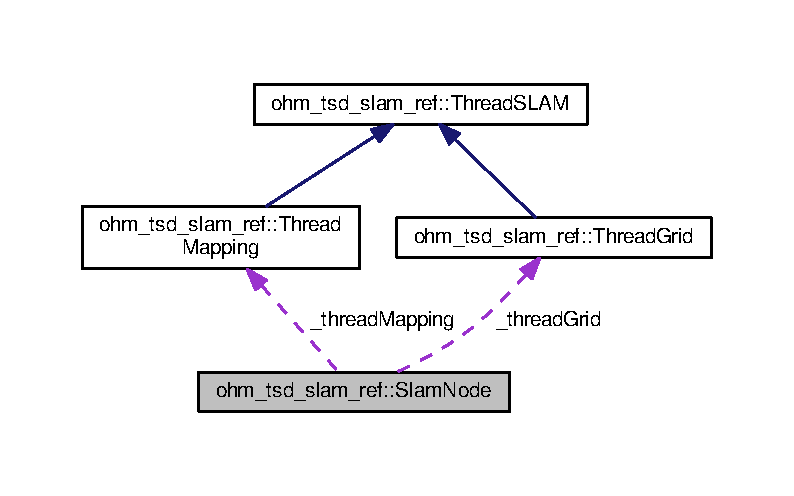
\includegraphics[width=350pt]{classohm__tsd__slam__ref_1_1SlamNode__coll__graph}
\end{center}
\end{figure}
\subsection*{Public Member Functions}
\begin{DoxyCompactItemize}
\item 
\hyperlink{classohm__tsd__slam__ref_1_1SlamNode_af35bd7adca13df47579a682ab3bb827d}{Slam\-Node} (void)
\begin{DoxyCompactList}\small\item\em Constructor. \end{DoxyCompactList}\item 
virtual \hyperlink{classohm__tsd__slam__ref_1_1SlamNode_a0dbbdf08b6ac75aba94c882715d7f49e}{$\sim$\-Slam\-Node} ()
\item 
void \hyperlink{classohm__tsd__slam__ref_1_1SlamNode_a4169535ecfeb3131a67efec9dea2f5c7}{start} (void)
\end{DoxyCompactItemize}
\subsection*{Private Member Functions}
\begin{DoxyCompactItemize}
\item 
void \hyperlink{classohm__tsd__slam__ref_1_1SlamNode_aac99efb88f38b6df5923f6a410f000a4}{run} (void)
\item 
void \hyperlink{classohm__tsd__slam__ref_1_1SlamNode_a21616e87819cf356088b8a2c9697451d}{timed\-Grid\-Pub} (void)
\item 
bool \hyperlink{classohm__tsd__slam__ref_1_1SlamNode_a5b4ee64a1d3b1ead996762adfc95ad94}{call\-Back\-Service\-Start\-Stop\-S\-L\-A\-M} (ohm\-\_\-tsd\-\_\-slam\-\_\-ref\-::\-Start\-Stop\-S\-L\-A\-M\-::\-Request \&req, ohm\-\_\-tsd\-\_\-slam\-\_\-ref\-::\-Start\-Stop\-S\-L\-A\-M\-::\-Response \&res)
\begin{DoxyCompactList}\small\item\em R\-O\-S service used for tilt scanner -\/ stops S\-L\-A\-M when tilt movement is ongoing. \end{DoxyCompactList}\end{DoxyCompactItemize}
\subsection*{Private Attributes}
\begin{DoxyCompactItemize}
\item 
ros\-::\-Node\-Handle \hyperlink{classohm__tsd__slam__ref_1_1SlamNode_a2e2b86d2d3ddff889a33152197e42894}{\-\_\-nh}
\item 
obvious\-::\-Tsd\-Grid $\ast$ \hyperlink{classohm__tsd__slam__ref_1_1SlamNode_a2b737790f425b4397bb7fb39373d4c3e}{\-\_\-grid}
\item 
\hyperlink{classohm__tsd__slam__ref_1_1ThreadMapping}{Thread\-Mapping} $\ast$ \hyperlink{classohm__tsd__slam__ref_1_1SlamNode_afdc6f1e42ee4910090dd49e84aa3cd82}{\-\_\-thread\-Mapping}
\item 
\hyperlink{classohm__tsd__slam__ref_1_1ThreadGrid}{Thread\-Grid} $\ast$ \hyperlink{classohm__tsd__slam__ref_1_1SlamNode_aa8894ed7f5c7413c1cfe5da64e3ac5b5}{\-\_\-thread\-Grid}
\item 
double \hyperlink{classohm__tsd__slam__ref_1_1SlamNode_ad57ec9810293549dc803209a950a776f}{\-\_\-x\-Off\-Factor}
\item 
double \hyperlink{classohm__tsd__slam__ref_1_1SlamNode_a591fdd2fc92e9fd53112b36f0125cf51}{\-\_\-y\-Off\-Factor}
\item 
ros\-::\-Duration $\ast$ \hyperlink{classohm__tsd__slam__ref_1_1SlamNode_a00ff10e215f1e307fca09351b25cc7c5}{\-\_\-grid\-Interval}
\item 
ros\-::\-Rate $\ast$ \hyperlink{classohm__tsd__slam__ref_1_1SlamNode_a09e9b76d84f565257c0aacda187c82ec}{\-\_\-loop\-Rate}
\item 
std\-::vector$<$ \hyperlink{structohm__tsd__slam__ref_1_1TaggedSubscriber}{Tagged\-Subscriber} $>$ \hyperlink{classohm__tsd__slam__ref_1_1SlamNode_a65b1147fbe5c773c55a7e2b640b77d01}{\-\_\-subs\-Laser}
\item 
std\-::vector$<$ \hyperlink{classohm__tsd__slam__ref_1_1ThreadLocalize}{Thread\-Localize} $\ast$ $>$ \hyperlink{classohm__tsd__slam__ref_1_1SlamNode_abe1e2022599a8ce220de76b142486ea8}{\-\_\-localizers}
\item 
ros\-::\-Service\-Server \hyperlink{classohm__tsd__slam__ref_1_1SlamNode_a2941b11fc25f02fad3467297f0260fec}{\-\_\-service\-Start\-Stop\-S\-L\-A\-M}
\end{DoxyCompactItemize}


\subsection{Detailed Description}
main node management of 2\-D slam, contains sub classes and ros interface 

\begin{DoxyAuthor}{Author}

\end{DoxyAuthor}


\subsection{Constructor \& Destructor Documentation}
\hypertarget{classohm__tsd__slam__ref_1_1SlamNode_af35bd7adca13df47579a682ab3bb827d}{\index{ohm\-\_\-tsd\-\_\-slam\-\_\-ref\-::\-Slam\-Node@{ohm\-\_\-tsd\-\_\-slam\-\_\-ref\-::\-Slam\-Node}!Slam\-Node@{Slam\-Node}}
\index{Slam\-Node@{Slam\-Node}!ohm_tsd_slam_ref::SlamNode@{ohm\-\_\-tsd\-\_\-slam\-\_\-ref\-::\-Slam\-Node}}
\subsubsection[{Slam\-Node}]{\setlength{\rightskip}{0pt plus 5cm}ohm\-\_\-tsd\-\_\-slam\-\_\-ref\-::\-Slam\-Node\-::\-Slam\-Node (
\begin{DoxyParamCaption}
\item[{void}]{}
\end{DoxyParamCaption}
)}}\label{classohm__tsd__slam__ref_1_1SlamNode_af35bd7adca13df47579a682ab3bb827d}


Constructor. 

class can be called in 2 modes, run\-Slam or run\-Localize (run method invoked by start method) default mode\-: S\-L\-A\-M mode, generates new empty obvious\-::\-Tsd\-Grid, dimension and resolution can be set by defines in \hyperlink{SlamNode_8h}{Slam\-Node.\-h} L\-O\-C\-A\-L\-I\-Z\-E mode\-: loads content from file at a given path, operates on a fixed model; in the fixed model no push into the grid is needed, no thread mapping (?richtig?) object is instantiated \begin{DoxyRefDesc}{Todo}
\item[\hyperlink{todo__todo000002}{Todo}]verwirrend \end{DoxyRefDesc}
\hypertarget{classohm__tsd__slam__ref_1_1SlamNode_a0dbbdf08b6ac75aba94c882715d7f49e}{\index{ohm\-\_\-tsd\-\_\-slam\-\_\-ref\-::\-Slam\-Node@{ohm\-\_\-tsd\-\_\-slam\-\_\-ref\-::\-Slam\-Node}!$\sim$\-Slam\-Node@{$\sim$\-Slam\-Node}}
\index{$\sim$\-Slam\-Node@{$\sim$\-Slam\-Node}!ohm_tsd_slam_ref::SlamNode@{ohm\-\_\-tsd\-\_\-slam\-\_\-ref\-::\-Slam\-Node}}
\subsubsection[{$\sim$\-Slam\-Node}]{\setlength{\rightskip}{0pt plus 5cm}ohm\-\_\-tsd\-\_\-slam\-\_\-ref\-::\-Slam\-Node\-::$\sim$\-Slam\-Node (
\begin{DoxyParamCaption}
{}
\end{DoxyParamCaption}
)\hspace{0.3cm}{\ttfamily [virtual]}}}\label{classohm__tsd__slam__ref_1_1SlamNode_a0dbbdf08b6ac75aba94c882715d7f49e}
Destructor stop all localization threads \begin{DoxyRefDesc}{Todo}
\item[\hyperlink{todo__todo000003}{Todo}]geht das so mit neuer foreach schleifn? prüfen, wenn \hyperlink{classohm__tsd__slam__ref_1_1ThreadLocalize}{Thread\-Localize} erstellt ist \end{DoxyRefDesc}


\subsection{Member Function Documentation}
\hypertarget{classohm__tsd__slam__ref_1_1SlamNode_a5b4ee64a1d3b1ead996762adfc95ad94}{\index{ohm\-\_\-tsd\-\_\-slam\-\_\-ref\-::\-Slam\-Node@{ohm\-\_\-tsd\-\_\-slam\-\_\-ref\-::\-Slam\-Node}!call\-Back\-Service\-Start\-Stop\-S\-L\-A\-M@{call\-Back\-Service\-Start\-Stop\-S\-L\-A\-M}}
\index{call\-Back\-Service\-Start\-Stop\-S\-L\-A\-M@{call\-Back\-Service\-Start\-Stop\-S\-L\-A\-M}!ohm_tsd_slam_ref::SlamNode@{ohm\-\_\-tsd\-\_\-slam\-\_\-ref\-::\-Slam\-Node}}
\subsubsection[{call\-Back\-Service\-Start\-Stop\-S\-L\-A\-M}]{\setlength{\rightskip}{0pt plus 5cm}bool ohm\-\_\-tsd\-\_\-slam\-\_\-ref\-::\-Slam\-Node\-::call\-Back\-Service\-Start\-Stop\-S\-L\-A\-M (
\begin{DoxyParamCaption}
\item[{ohm\-\_\-tsd\-\_\-slam\-\_\-ref\-::\-Start\-Stop\-S\-L\-A\-M\-::\-Request \&}]{req, }
\item[{ohm\-\_\-tsd\-\_\-slam\-\_\-ref\-::\-Start\-Stop\-S\-L\-A\-M\-::\-Response \&}]{res}
\end{DoxyParamCaption}
)\hspace{0.3cm}{\ttfamily [private]}}}\label{classohm__tsd__slam__ref_1_1SlamNode_a5b4ee64a1d3b1ead996762adfc95ad94}


R\-O\-S service used for tilt scanner -\/ stops S\-L\-A\-M when tilt movement is ongoing. 


\begin{DoxyParams}{Parameters}
{\em req} & R\-O\-S service request \\
\hline
{\em res} & R\-O\-S service response \\
\hline
\end{DoxyParams}
\begin{DoxyReturn}{Returns}

\end{DoxyReturn}
\begin{DoxyRefDesc}{Todo}
\item[\hyperlink{todo__todo000011}{Todo}]nachfragen \end{DoxyRefDesc}
\hypertarget{classohm__tsd__slam__ref_1_1SlamNode_aac99efb88f38b6df5923f6a410f000a4}{\index{ohm\-\_\-tsd\-\_\-slam\-\_\-ref\-::\-Slam\-Node@{ohm\-\_\-tsd\-\_\-slam\-\_\-ref\-::\-Slam\-Node}!run@{run}}
\index{run@{run}!ohm_tsd_slam_ref::SlamNode@{ohm\-\_\-tsd\-\_\-slam\-\_\-ref\-::\-Slam\-Node}}
\subsubsection[{run}]{\setlength{\rightskip}{0pt plus 5cm}void ohm\-\_\-tsd\-\_\-slam\-\_\-ref\-::\-Slam\-Node\-::run (
\begin{DoxyParamCaption}
\item[{void}]{}
\end{DoxyParamCaption}
)\hspace{0.3cm}{\ttfamily [private]}}}\label{classohm__tsd__slam__ref_1_1SlamNode_aac99efb88f38b6df5923f6a410f000a4}
main slam method including ros\-::spin\-Once etc. calls \hyperlink{classohm__tsd__slam__ref_1_1SlamNode_a21616e87819cf356088b8a2c9697451d}{timed\-Grid\-Pub()} \hypertarget{classohm__tsd__slam__ref_1_1SlamNode_a4169535ecfeb3131a67efec9dea2f5c7}{\index{ohm\-\_\-tsd\-\_\-slam\-\_\-ref\-::\-Slam\-Node@{ohm\-\_\-tsd\-\_\-slam\-\_\-ref\-::\-Slam\-Node}!start@{start}}
\index{start@{start}!ohm_tsd_slam_ref::SlamNode@{ohm\-\_\-tsd\-\_\-slam\-\_\-ref\-::\-Slam\-Node}}
\subsubsection[{start}]{\setlength{\rightskip}{0pt plus 5cm}void ohm\-\_\-tsd\-\_\-slam\-\_\-ref\-::\-Slam\-Node\-::start (
\begin{DoxyParamCaption}
\item[{void}]{}
\end{DoxyParamCaption}
)\hspace{0.3cm}{\ttfamily [inline]}}}\label{classohm__tsd__slam__ref_1_1SlamNode_a4169535ecfeb3131a67efec9dea2f5c7}
called in main function to start \hyperlink{classohm__tsd__slam__ref_1_1SlamNode}{Slam\-Node} calls \hyperlink{classohm__tsd__slam__ref_1_1SlamNode_aac99efb88f38b6df5923f6a410f000a4}{run()} method which defines the mode, S\-L\-A\-M or L\-O\-C\-A\-L\-I\-Z\-E \hypertarget{classohm__tsd__slam__ref_1_1SlamNode_a21616e87819cf356088b8a2c9697451d}{\index{ohm\-\_\-tsd\-\_\-slam\-\_\-ref\-::\-Slam\-Node@{ohm\-\_\-tsd\-\_\-slam\-\_\-ref\-::\-Slam\-Node}!timed\-Grid\-Pub@{timed\-Grid\-Pub}}
\index{timed\-Grid\-Pub@{timed\-Grid\-Pub}!ohm_tsd_slam_ref::SlamNode@{ohm\-\_\-tsd\-\_\-slam\-\_\-ref\-::\-Slam\-Node}}
\subsubsection[{timed\-Grid\-Pub}]{\setlength{\rightskip}{0pt plus 5cm}void ohm\-\_\-tsd\-\_\-slam\-\_\-ref\-::\-Slam\-Node\-::timed\-Grid\-Pub (
\begin{DoxyParamCaption}
\item[{void}]{}
\end{DoxyParamCaption}
)\hspace{0.3cm}{\ttfamily [private]}}}\label{classohm__tsd__slam__ref_1_1SlamNode_a21616e87819cf356088b8a2c9697451d}
calculates time difference between last map and now calls unblock() method of class \hyperlink{classohm__tsd__slam__ref_1_1ThreadSLAM}{Thread\-S\-L\-A\-M} -\/ to enable occupancy grid thread with certain frequency if time difference $>$ \-\_\-grid\-Interval (\char`\"{}thresh\char`\"{} -\/ rate used for occupancy grid generation) 

\subsection{Member Data Documentation}
\hypertarget{classohm__tsd__slam__ref_1_1SlamNode_a2b737790f425b4397bb7fb39373d4c3e}{\index{ohm\-\_\-tsd\-\_\-slam\-\_\-ref\-::\-Slam\-Node@{ohm\-\_\-tsd\-\_\-slam\-\_\-ref\-::\-Slam\-Node}!\-\_\-grid@{\-\_\-grid}}
\index{\-\_\-grid@{\-\_\-grid}!ohm_tsd_slam_ref::SlamNode@{ohm\-\_\-tsd\-\_\-slam\-\_\-ref\-::\-Slam\-Node}}
\subsubsection[{\-\_\-grid}]{\setlength{\rightskip}{0pt plus 5cm}obvious\-::\-Tsd\-Grid$\ast$ ohm\-\_\-tsd\-\_\-slam\-\_\-ref\-::\-Slam\-Node\-::\-\_\-grid\hspace{0.3cm}{\ttfamily [private]}}}\label{classohm__tsd__slam__ref_1_1SlamNode_a2b737790f425b4397bb7fb39373d4c3e}
Representation -\/ instance of one Tsd\-Grid \hypertarget{classohm__tsd__slam__ref_1_1SlamNode_a00ff10e215f1e307fca09351b25cc7c5}{\index{ohm\-\_\-tsd\-\_\-slam\-\_\-ref\-::\-Slam\-Node@{ohm\-\_\-tsd\-\_\-slam\-\_\-ref\-::\-Slam\-Node}!\-\_\-grid\-Interval@{\-\_\-grid\-Interval}}
\index{\-\_\-grid\-Interval@{\-\_\-grid\-Interval}!ohm_tsd_slam_ref::SlamNode@{ohm\-\_\-tsd\-\_\-slam\-\_\-ref\-::\-Slam\-Node}}
\subsubsection[{\-\_\-grid\-Interval}]{\setlength{\rightskip}{0pt plus 5cm}ros\-::\-Duration$\ast$ ohm\-\_\-tsd\-\_\-slam\-\_\-ref\-::\-Slam\-Node\-::\-\_\-grid\-Interval\hspace{0.3cm}{\ttfamily [private]}}}\label{classohm__tsd__slam__ref_1_1SlamNode_a00ff10e215f1e307fca09351b25cc7c5}
Rate used for occupancy grid generation Minimum time interval for new grid pub -\/ if time between last pub and now is greater than \-\_\-grid\-Interval -\/ new occ grid pub \hypertarget{classohm__tsd__slam__ref_1_1SlamNode_abe1e2022599a8ce220de76b142486ea8}{\index{ohm\-\_\-tsd\-\_\-slam\-\_\-ref\-::\-Slam\-Node@{ohm\-\_\-tsd\-\_\-slam\-\_\-ref\-::\-Slam\-Node}!\-\_\-localizers@{\-\_\-localizers}}
\index{\-\_\-localizers@{\-\_\-localizers}!ohm_tsd_slam_ref::SlamNode@{ohm\-\_\-tsd\-\_\-slam\-\_\-ref\-::\-Slam\-Node}}
\subsubsection[{\-\_\-localizers}]{\setlength{\rightskip}{0pt plus 5cm}std\-::vector$<${\bf Thread\-Localize}$\ast$$>$ ohm\-\_\-tsd\-\_\-slam\-\_\-ref\-::\-Slam\-Node\-::\-\_\-localizers\hspace{0.3cm}{\ttfamily [private]}}}\label{classohm__tsd__slam__ref_1_1SlamNode_abe1e2022599a8ce220de76b142486ea8}
\begin{DoxyRefDesc}{Todo}
\item[\hyperlink{todo__todo000014}{Todo}]was macht das hier? storing \-\_\-grid, \-\_\-thread\-Mapping, x\-Offset and y\-Offset of \hyperlink{classohm__tsd__slam__ref_1_1ThreadLocalize}{Thread\-Localize} \end{DoxyRefDesc}
\hypertarget{classohm__tsd__slam__ref_1_1SlamNode_a09e9b76d84f565257c0aacda187c82ec}{\index{ohm\-\_\-tsd\-\_\-slam\-\_\-ref\-::\-Slam\-Node@{ohm\-\_\-tsd\-\_\-slam\-\_\-ref\-::\-Slam\-Node}!\-\_\-loop\-Rate@{\-\_\-loop\-Rate}}
\index{\-\_\-loop\-Rate@{\-\_\-loop\-Rate}!ohm_tsd_slam_ref::SlamNode@{ohm\-\_\-tsd\-\_\-slam\-\_\-ref\-::\-Slam\-Node}}
\subsubsection[{\-\_\-loop\-Rate}]{\setlength{\rightskip}{0pt plus 5cm}ros\-::\-Rate$\ast$ ohm\-\_\-tsd\-\_\-slam\-\_\-ref\-::\-Slam\-Node\-::\-\_\-loop\-Rate\hspace{0.3cm}{\ttfamily [private]}}}\label{classohm__tsd__slam__ref_1_1SlamNode_a09e9b76d84f565257c0aacda187c82ec}
Desired loop rate \hypertarget{classohm__tsd__slam__ref_1_1SlamNode_a2e2b86d2d3ddff889a33152197e42894}{\index{ohm\-\_\-tsd\-\_\-slam\-\_\-ref\-::\-Slam\-Node@{ohm\-\_\-tsd\-\_\-slam\-\_\-ref\-::\-Slam\-Node}!\-\_\-nh@{\-\_\-nh}}
\index{\-\_\-nh@{\-\_\-nh}!ohm_tsd_slam_ref::SlamNode@{ohm\-\_\-tsd\-\_\-slam\-\_\-ref\-::\-Slam\-Node}}
\subsubsection[{\-\_\-nh}]{\setlength{\rightskip}{0pt plus 5cm}ros\-::\-Node\-Handle ohm\-\_\-tsd\-\_\-slam\-\_\-ref\-::\-Slam\-Node\-::\-\_\-nh\hspace{0.3cm}{\ttfamily [private]}}}\label{classohm__tsd__slam__ref_1_1SlamNode_a2e2b86d2d3ddff889a33152197e42894}
Main node handle \hypertarget{classohm__tsd__slam__ref_1_1SlamNode_a2941b11fc25f02fad3467297f0260fec}{\index{ohm\-\_\-tsd\-\_\-slam\-\_\-ref\-::\-Slam\-Node@{ohm\-\_\-tsd\-\_\-slam\-\_\-ref\-::\-Slam\-Node}!\-\_\-service\-Start\-Stop\-S\-L\-A\-M@{\-\_\-service\-Start\-Stop\-S\-L\-A\-M}}
\index{\-\_\-service\-Start\-Stop\-S\-L\-A\-M@{\-\_\-service\-Start\-Stop\-S\-L\-A\-M}!ohm_tsd_slam_ref::SlamNode@{ohm\-\_\-tsd\-\_\-slam\-\_\-ref\-::\-Slam\-Node}}
\subsubsection[{\-\_\-service\-Start\-Stop\-S\-L\-A\-M}]{\setlength{\rightskip}{0pt plus 5cm}ros\-::\-Service\-Server ohm\-\_\-tsd\-\_\-slam\-\_\-ref\-::\-Slam\-Node\-::\-\_\-service\-Start\-Stop\-S\-L\-A\-M\hspace{0.3cm}{\ttfamily [private]}}}\label{classohm__tsd__slam__ref_1_1SlamNode_a2941b11fc25f02fad3467297f0260fec}
\begin{DoxyRefDesc}{Todo}
\item[\hyperlink{todo__todo000015}{Todo}]wofür brauchen wir den service? \end{DoxyRefDesc}
\hypertarget{classohm__tsd__slam__ref_1_1SlamNode_a65b1147fbe5c773c55a7e2b640b77d01}{\index{ohm\-\_\-tsd\-\_\-slam\-\_\-ref\-::\-Slam\-Node@{ohm\-\_\-tsd\-\_\-slam\-\_\-ref\-::\-Slam\-Node}!\-\_\-subs\-Laser@{\-\_\-subs\-Laser}}
\index{\-\_\-subs\-Laser@{\-\_\-subs\-Laser}!ohm_tsd_slam_ref::SlamNode@{ohm\-\_\-tsd\-\_\-slam\-\_\-ref\-::\-Slam\-Node}}
\subsubsection[{\-\_\-subs\-Laser}]{\setlength{\rightskip}{0pt plus 5cm}std\-::vector$<${\bf Tagged\-Subscriber}$>$ ohm\-\_\-tsd\-\_\-slam\-\_\-ref\-::\-Slam\-Node\-::\-\_\-subs\-Laser\hspace{0.3cm}{\ttfamily [private]}}}\label{classohm__tsd__slam__ref_1_1SlamNode_a65b1147fbe5c773c55a7e2b640b77d01}
R\-O\-S laser subscriber, storing all laser beams in a vector \hypertarget{classohm__tsd__slam__ref_1_1SlamNode_aa8894ed7f5c7413c1cfe5da64e3ac5b5}{\index{ohm\-\_\-tsd\-\_\-slam\-\_\-ref\-::\-Slam\-Node@{ohm\-\_\-tsd\-\_\-slam\-\_\-ref\-::\-Slam\-Node}!\-\_\-thread\-Grid@{\-\_\-thread\-Grid}}
\index{\-\_\-thread\-Grid@{\-\_\-thread\-Grid}!ohm_tsd_slam_ref::SlamNode@{ohm\-\_\-tsd\-\_\-slam\-\_\-ref\-::\-Slam\-Node}}
\subsubsection[{\-\_\-thread\-Grid}]{\setlength{\rightskip}{0pt plus 5cm}{\bf Thread\-Grid}$\ast$ ohm\-\_\-tsd\-\_\-slam\-\_\-ref\-::\-Slam\-Node\-::\-\_\-thread\-Grid\hspace{0.3cm}{\ttfamily [private]}}}\label{classohm__tsd__slam__ref_1_1SlamNode_aa8894ed7f5c7413c1cfe5da64e3ac5b5}
Grid thread instance of class \hyperlink{classohm__tsd__slam__ref_1_1ThreadGrid}{Thread\-Grid} \hypertarget{classohm__tsd__slam__ref_1_1SlamNode_afdc6f1e42ee4910090dd49e84aa3cd82}{\index{ohm\-\_\-tsd\-\_\-slam\-\_\-ref\-::\-Slam\-Node@{ohm\-\_\-tsd\-\_\-slam\-\_\-ref\-::\-Slam\-Node}!\-\_\-thread\-Mapping@{\-\_\-thread\-Mapping}}
\index{\-\_\-thread\-Mapping@{\-\_\-thread\-Mapping}!ohm_tsd_slam_ref::SlamNode@{ohm\-\_\-tsd\-\_\-slam\-\_\-ref\-::\-Slam\-Node}}
\subsubsection[{\-\_\-thread\-Mapping}]{\setlength{\rightskip}{0pt plus 5cm}{\bf Thread\-Mapping}$\ast$ ohm\-\_\-tsd\-\_\-slam\-\_\-ref\-::\-Slam\-Node\-::\-\_\-thread\-Mapping\hspace{0.3cm}{\ttfamily [private]}}}\label{classohm__tsd__slam__ref_1_1SlamNode_afdc6f1e42ee4910090dd49e84aa3cd82}
Create Mapping thread instance of class \hyperlink{classohm__tsd__slam__ref_1_1ThreadMapping}{Thread\-Mapping} \hypertarget{classohm__tsd__slam__ref_1_1SlamNode_ad57ec9810293549dc803209a950a776f}{\index{ohm\-\_\-tsd\-\_\-slam\-\_\-ref\-::\-Slam\-Node@{ohm\-\_\-tsd\-\_\-slam\-\_\-ref\-::\-Slam\-Node}!\-\_\-x\-Off\-Factor@{\-\_\-x\-Off\-Factor}}
\index{\-\_\-x\-Off\-Factor@{\-\_\-x\-Off\-Factor}!ohm_tsd_slam_ref::SlamNode@{ohm\-\_\-tsd\-\_\-slam\-\_\-ref\-::\-Slam\-Node}}
\subsubsection[{\-\_\-x\-Off\-Factor}]{\setlength{\rightskip}{0pt plus 5cm}double ohm\-\_\-tsd\-\_\-slam\-\_\-ref\-::\-Slam\-Node\-::\-\_\-x\-Off\-Factor\hspace{0.3cm}{\ttfamily [private]}}}\label{classohm__tsd__slam__ref_1_1SlamNode_ad57ec9810293549dc803209a950a776f}
X starting offset factor \begin{DoxyRefDesc}{Todo}
\item[\hyperlink{todo__todo000012}{Todo}]same as \-\_\-x\-Off\-Factor -\/ prüfen, glaub das wird nicht verwendet -- launch file params auch löschen \end{DoxyRefDesc}
\hypertarget{classohm__tsd__slam__ref_1_1SlamNode_a591fdd2fc92e9fd53112b36f0125cf51}{\index{ohm\-\_\-tsd\-\_\-slam\-\_\-ref\-::\-Slam\-Node@{ohm\-\_\-tsd\-\_\-slam\-\_\-ref\-::\-Slam\-Node}!\-\_\-y\-Off\-Factor@{\-\_\-y\-Off\-Factor}}
\index{\-\_\-y\-Off\-Factor@{\-\_\-y\-Off\-Factor}!ohm_tsd_slam_ref::SlamNode@{ohm\-\_\-tsd\-\_\-slam\-\_\-ref\-::\-Slam\-Node}}
\subsubsection[{\-\_\-y\-Off\-Factor}]{\setlength{\rightskip}{0pt plus 5cm}double ohm\-\_\-tsd\-\_\-slam\-\_\-ref\-::\-Slam\-Node\-::\-\_\-y\-Off\-Factor\hspace{0.3cm}{\ttfamily [private]}}}\label{classohm__tsd__slam__ref_1_1SlamNode_a591fdd2fc92e9fd53112b36f0125cf51}
Y starting offset factor \begin{DoxyRefDesc}{Todo}
\item[\hyperlink{todo__todo000013}{Todo}]wofür gibt es die offset factors? im slamnode.\-cpp definier ich ja nochmal launch file params für x\-Offset u y\-Offset -\/ sehe keine Verwendung von \-\_\-y\-Off\-Factor 

prüfen, glaub das wird nicht verwendet -- launch file params auch löschen \end{DoxyRefDesc}


The documentation for this class was generated from the following files\-:\begin{DoxyCompactItemize}
\item 
src/\hyperlink{SlamNode_8h}{Slam\-Node.\-h}\item 
src/\hyperlink{SlamNode_8cpp}{Slam\-Node.\-cpp}\end{DoxyCompactItemize}

\hypertarget{structohm__tsd__slam__ref_1_1TaggedSubscriber}{\section{ohm\-\_\-tsd\-\_\-slam\-\_\-ref\-:\-:Tagged\-Subscriber Struct Reference}
\label{structohm__tsd__slam__ref_1_1TaggedSubscriber}\index{ohm\-\_\-tsd\-\_\-slam\-\_\-ref\-::\-Tagged\-Subscriber@{ohm\-\_\-tsd\-\_\-slam\-\_\-ref\-::\-Tagged\-Subscriber}}
}


\hyperlink{structohm__tsd__slam__ref_1_1TaggedSubscriber}{Tagged\-Subscriber} struct creates new datatype of subscribers for ros communication.  




{\ttfamily \#include $<$Slam\-Node.\-h$>$}



Collaboration diagram for ohm\-\_\-tsd\-\_\-slam\-\_\-ref\-:\-:Tagged\-Subscriber\-:\nopagebreak
\begin{figure}[H]
\begin{center}
\leavevmode
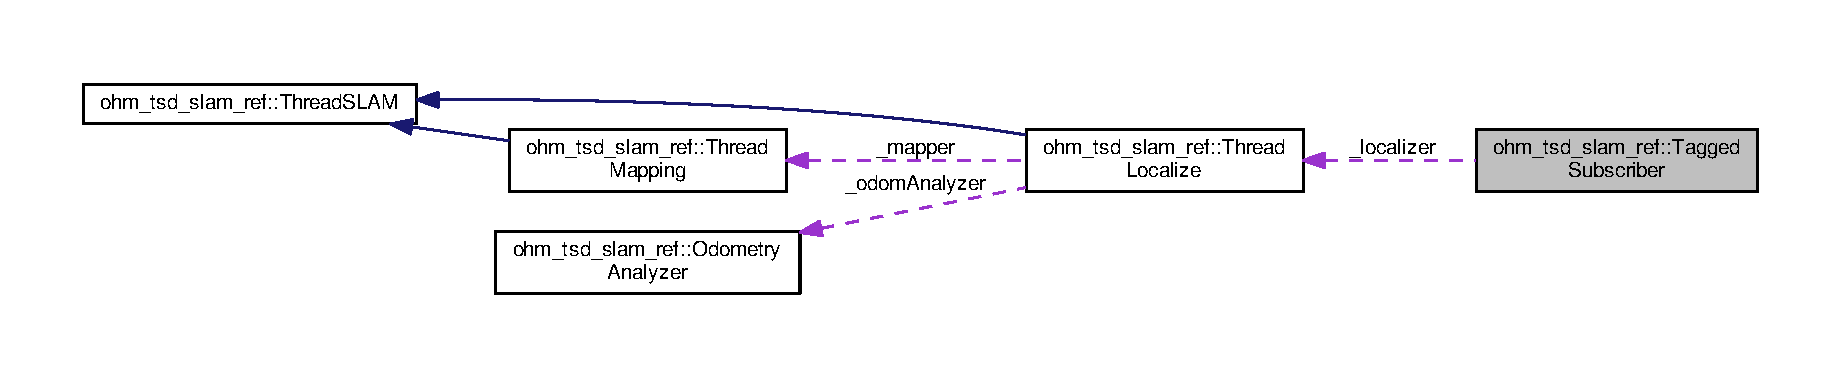
\includegraphics[width=350pt]{structohm__tsd__slam__ref_1_1TaggedSubscriber__coll__graph}
\end{center}
\end{figure}
\subsection*{Public Member Functions}
\begin{DoxyCompactItemize}
\item 
\hyperlink{structohm__tsd__slam__ref_1_1TaggedSubscriber_aa27ec1bb6608bfa803165eb92bf46135}{Tagges\-Subscriber} (std\-::string \hyperlink{structohm__tsd__slam__ref_1_1TaggedSubscriber_a6d4ad13158333a16725cdc1cdd6ab3c2}{topic}, \hyperlink{classohm__tsd__slam__ref_1_1ThreadLocalize}{Thread\-Localize} \&localizer, ros\-::\-Node\-Handle \&nh)
\item 
\hyperlink{structohm__tsd__slam__ref_1_1TaggedSubscriber_aac3521e675e9be4b0d68b96fb7782060}{Tagged\-Subscriber} (const \hyperlink{structohm__tsd__slam__ref_1_1TaggedSubscriber}{Tagged\-Subscriber} \&subs)
\item 
\hyperlink{structohm__tsd__slam__ref_1_1TaggedSubscriber_af58c6641892429bd5d21bdcc5f8f373a}{Tagged\-Subscriber} (void)
\item 
void \hyperlink{structohm__tsd__slam__ref_1_1TaggedSubscriber_a6d95060dc96fb1069588d681668e1420}{switch\-On} (void)
\item 
void \hyperlink{structohm__tsd__slam__ref_1_1TaggedSubscriber_ac41328ef3bb26e0f000f12c989aaf849}{switch\-Off} (void)
\item 
bool \hyperlink{structohm__tsd__slam__ref_1_1TaggedSubscriber_a6d4ad13158333a16725cdc1cdd6ab3c2}{topic} (const std\-::string topic)
\end{DoxyCompactItemize}
\subsection*{Public Attributes}
\begin{DoxyCompactItemize}
\item 
ros\-::\-Subscriber \hyperlink{structohm__tsd__slam__ref_1_1TaggedSubscriber_a61345fb4c4b4e617dfffe70b5b1bd60c}{\-\_\-subs}
\item 
std\-::string \hyperlink{structohm__tsd__slam__ref_1_1TaggedSubscriber_a768a784062a20f2e9a11a1b528c11605}{\-\_\-topic}
\item 
\hyperlink{classohm__tsd__slam__ref_1_1ThreadLocalize}{Thread\-Localize} $\ast$ \hyperlink{structohm__tsd__slam__ref_1_1TaggedSubscriber_afe33f4a8274392173ea2a4ff05f49bc4}{\-\_\-localizer}
\item 
ros\-::\-Node\-Handle \hyperlink{structohm__tsd__slam__ref_1_1TaggedSubscriber_a0ff0c67d13bf2c9c606c25ffa24db8df}{\-\_\-nh}
\end{DoxyCompactItemize}


\subsection{Detailed Description}
\hyperlink{structohm__tsd__slam__ref_1_1TaggedSubscriber}{Tagged\-Subscriber} struct creates new datatype of subscribers for ros communication. 

\begin{DoxyRefDesc}{Todo}
\item[\hyperlink{todo__todo000009}{Todo}]nachfragen \end{DoxyRefDesc}


\subsection{Constructor \& Destructor Documentation}
\hypertarget{structohm__tsd__slam__ref_1_1TaggedSubscriber_aac3521e675e9be4b0d68b96fb7782060}{\index{ohm\-\_\-tsd\-\_\-slam\-\_\-ref\-::\-Tagged\-Subscriber@{ohm\-\_\-tsd\-\_\-slam\-\_\-ref\-::\-Tagged\-Subscriber}!Tagged\-Subscriber@{Tagged\-Subscriber}}
\index{Tagged\-Subscriber@{Tagged\-Subscriber}!ohm_tsd_slam_ref::TaggedSubscriber@{ohm\-\_\-tsd\-\_\-slam\-\_\-ref\-::\-Tagged\-Subscriber}}
\subsubsection[{Tagged\-Subscriber}]{\setlength{\rightskip}{0pt plus 5cm}ohm\-\_\-tsd\-\_\-slam\-\_\-ref\-::\-Tagged\-Subscriber\-::\-Tagged\-Subscriber (
\begin{DoxyParamCaption}
\item[{const {\bf Tagged\-Subscriber} \&}]{subs}
\end{DoxyParamCaption}
)\hspace{0.3cm}{\ttfamily [inline]}}}\label{structohm__tsd__slam__ref_1_1TaggedSubscriber_aac3521e675e9be4b0d68b96fb7782060}
\hypertarget{structohm__tsd__slam__ref_1_1TaggedSubscriber_af58c6641892429bd5d21bdcc5f8f373a}{\index{ohm\-\_\-tsd\-\_\-slam\-\_\-ref\-::\-Tagged\-Subscriber@{ohm\-\_\-tsd\-\_\-slam\-\_\-ref\-::\-Tagged\-Subscriber}!Tagged\-Subscriber@{Tagged\-Subscriber}}
\index{Tagged\-Subscriber@{Tagged\-Subscriber}!ohm_tsd_slam_ref::TaggedSubscriber@{ohm\-\_\-tsd\-\_\-slam\-\_\-ref\-::\-Tagged\-Subscriber}}
\subsubsection[{Tagged\-Subscriber}]{\setlength{\rightskip}{0pt plus 5cm}ohm\-\_\-tsd\-\_\-slam\-\_\-ref\-::\-Tagged\-Subscriber\-::\-Tagged\-Subscriber (
\begin{DoxyParamCaption}
\item[{void}]{}
\end{DoxyParamCaption}
)\hspace{0.3cm}{\ttfamily [inline]}}}\label{structohm__tsd__slam__ref_1_1TaggedSubscriber_af58c6641892429bd5d21bdcc5f8f373a}


\subsection{Member Function Documentation}
\hypertarget{structohm__tsd__slam__ref_1_1TaggedSubscriber_ac41328ef3bb26e0f000f12c989aaf849}{\index{ohm\-\_\-tsd\-\_\-slam\-\_\-ref\-::\-Tagged\-Subscriber@{ohm\-\_\-tsd\-\_\-slam\-\_\-ref\-::\-Tagged\-Subscriber}!switch\-Off@{switch\-Off}}
\index{switch\-Off@{switch\-Off}!ohm_tsd_slam_ref::TaggedSubscriber@{ohm\-\_\-tsd\-\_\-slam\-\_\-ref\-::\-Tagged\-Subscriber}}
\subsubsection[{switch\-Off}]{\setlength{\rightskip}{0pt plus 5cm}void ohm\-\_\-tsd\-\_\-slam\-\_\-ref\-::\-Tagged\-Subscriber\-::switch\-Off (
\begin{DoxyParamCaption}
\item[{void}]{}
\end{DoxyParamCaption}
)\hspace{0.3cm}{\ttfamily [inline]}}}\label{structohm__tsd__slam__ref_1_1TaggedSubscriber_ac41328ef3bb26e0f000f12c989aaf849}
\hypertarget{structohm__tsd__slam__ref_1_1TaggedSubscriber_a6d95060dc96fb1069588d681668e1420}{\index{ohm\-\_\-tsd\-\_\-slam\-\_\-ref\-::\-Tagged\-Subscriber@{ohm\-\_\-tsd\-\_\-slam\-\_\-ref\-::\-Tagged\-Subscriber}!switch\-On@{switch\-On}}
\index{switch\-On@{switch\-On}!ohm_tsd_slam_ref::TaggedSubscriber@{ohm\-\_\-tsd\-\_\-slam\-\_\-ref\-::\-Tagged\-Subscriber}}
\subsubsection[{switch\-On}]{\setlength{\rightskip}{0pt plus 5cm}void ohm\-\_\-tsd\-\_\-slam\-\_\-ref\-::\-Tagged\-Subscriber\-::switch\-On (
\begin{DoxyParamCaption}
\item[{void}]{}
\end{DoxyParamCaption}
)\hspace{0.3cm}{\ttfamily [inline]}}}\label{structohm__tsd__slam__ref_1_1TaggedSubscriber_a6d95060dc96fb1069588d681668e1420}
\hypertarget{structohm__tsd__slam__ref_1_1TaggedSubscriber_aa27ec1bb6608bfa803165eb92bf46135}{\index{ohm\-\_\-tsd\-\_\-slam\-\_\-ref\-::\-Tagged\-Subscriber@{ohm\-\_\-tsd\-\_\-slam\-\_\-ref\-::\-Tagged\-Subscriber}!Tagges\-Subscriber@{Tagges\-Subscriber}}
\index{Tagges\-Subscriber@{Tagges\-Subscriber}!ohm_tsd_slam_ref::TaggedSubscriber@{ohm\-\_\-tsd\-\_\-slam\-\_\-ref\-::\-Tagged\-Subscriber}}
\subsubsection[{Tagges\-Subscriber}]{\setlength{\rightskip}{0pt plus 5cm}ohm\-\_\-tsd\-\_\-slam\-\_\-ref\-::\-Tagged\-Subscriber\-::\-Tagges\-Subscriber (
\begin{DoxyParamCaption}
\item[{std\-::string}]{topic, }
\item[{{\bf Thread\-Localize} \&}]{localizer, }
\item[{ros\-::\-Node\-Handle \&}]{nh}
\end{DoxyParamCaption}
)\hspace{0.3cm}{\ttfamily [inline]}}}\label{structohm__tsd__slam__ref_1_1TaggedSubscriber_aa27ec1bb6608bfa803165eb92bf46135}
\hypertarget{structohm__tsd__slam__ref_1_1TaggedSubscriber_a6d4ad13158333a16725cdc1cdd6ab3c2}{\index{ohm\-\_\-tsd\-\_\-slam\-\_\-ref\-::\-Tagged\-Subscriber@{ohm\-\_\-tsd\-\_\-slam\-\_\-ref\-::\-Tagged\-Subscriber}!topic@{topic}}
\index{topic@{topic}!ohm_tsd_slam_ref::TaggedSubscriber@{ohm\-\_\-tsd\-\_\-slam\-\_\-ref\-::\-Tagged\-Subscriber}}
\subsubsection[{topic}]{\setlength{\rightskip}{0pt plus 5cm}bool ohm\-\_\-tsd\-\_\-slam\-\_\-ref\-::\-Tagged\-Subscriber\-::topic (
\begin{DoxyParamCaption}
\item[{const std\-::string}]{topic}
\end{DoxyParamCaption}
)\hspace{0.3cm}{\ttfamily [inline]}}}\label{structohm__tsd__slam__ref_1_1TaggedSubscriber_a6d4ad13158333a16725cdc1cdd6ab3c2}
\begin{DoxyRefDesc}{Todo}
\item[\hyperlink{todo__todo000010}{Todo}]was macht bool topic fct? \end{DoxyRefDesc}


\subsection{Member Data Documentation}
\hypertarget{structohm__tsd__slam__ref_1_1TaggedSubscriber_afe33f4a8274392173ea2a4ff05f49bc4}{\index{ohm\-\_\-tsd\-\_\-slam\-\_\-ref\-::\-Tagged\-Subscriber@{ohm\-\_\-tsd\-\_\-slam\-\_\-ref\-::\-Tagged\-Subscriber}!\-\_\-localizer@{\-\_\-localizer}}
\index{\-\_\-localizer@{\-\_\-localizer}!ohm_tsd_slam_ref::TaggedSubscriber@{ohm\-\_\-tsd\-\_\-slam\-\_\-ref\-::\-Tagged\-Subscriber}}
\subsubsection[{\-\_\-localizer}]{\setlength{\rightskip}{0pt plus 5cm}{\bf Thread\-Localize}$\ast$ ohm\-\_\-tsd\-\_\-slam\-\_\-ref\-::\-Tagged\-Subscriber\-::\-\_\-localizer}}\label{structohm__tsd__slam__ref_1_1TaggedSubscriber_afe33f4a8274392173ea2a4ff05f49bc4}
\hypertarget{structohm__tsd__slam__ref_1_1TaggedSubscriber_a0ff0c67d13bf2c9c606c25ffa24db8df}{\index{ohm\-\_\-tsd\-\_\-slam\-\_\-ref\-::\-Tagged\-Subscriber@{ohm\-\_\-tsd\-\_\-slam\-\_\-ref\-::\-Tagged\-Subscriber}!\-\_\-nh@{\-\_\-nh}}
\index{\-\_\-nh@{\-\_\-nh}!ohm_tsd_slam_ref::TaggedSubscriber@{ohm\-\_\-tsd\-\_\-slam\-\_\-ref\-::\-Tagged\-Subscriber}}
\subsubsection[{\-\_\-nh}]{\setlength{\rightskip}{0pt plus 5cm}ros\-::\-Node\-Handle ohm\-\_\-tsd\-\_\-slam\-\_\-ref\-::\-Tagged\-Subscriber\-::\-\_\-nh}}\label{structohm__tsd__slam__ref_1_1TaggedSubscriber_a0ff0c67d13bf2c9c606c25ffa24db8df}
\hypertarget{structohm__tsd__slam__ref_1_1TaggedSubscriber_a61345fb4c4b4e617dfffe70b5b1bd60c}{\index{ohm\-\_\-tsd\-\_\-slam\-\_\-ref\-::\-Tagged\-Subscriber@{ohm\-\_\-tsd\-\_\-slam\-\_\-ref\-::\-Tagged\-Subscriber}!\-\_\-subs@{\-\_\-subs}}
\index{\-\_\-subs@{\-\_\-subs}!ohm_tsd_slam_ref::TaggedSubscriber@{ohm\-\_\-tsd\-\_\-slam\-\_\-ref\-::\-Tagged\-Subscriber}}
\subsubsection[{\-\_\-subs}]{\setlength{\rightskip}{0pt plus 5cm}ros\-::\-Subscriber ohm\-\_\-tsd\-\_\-slam\-\_\-ref\-::\-Tagged\-Subscriber\-::\-\_\-subs}}\label{structohm__tsd__slam__ref_1_1TaggedSubscriber_a61345fb4c4b4e617dfffe70b5b1bd60c}
\hypertarget{structohm__tsd__slam__ref_1_1TaggedSubscriber_a768a784062a20f2e9a11a1b528c11605}{\index{ohm\-\_\-tsd\-\_\-slam\-\_\-ref\-::\-Tagged\-Subscriber@{ohm\-\_\-tsd\-\_\-slam\-\_\-ref\-::\-Tagged\-Subscriber}!\-\_\-topic@{\-\_\-topic}}
\index{\-\_\-topic@{\-\_\-topic}!ohm_tsd_slam_ref::TaggedSubscriber@{ohm\-\_\-tsd\-\_\-slam\-\_\-ref\-::\-Tagged\-Subscriber}}
\subsubsection[{\-\_\-topic}]{\setlength{\rightskip}{0pt plus 5cm}std\-::string ohm\-\_\-tsd\-\_\-slam\-\_\-ref\-::\-Tagged\-Subscriber\-::\-\_\-topic}}\label{structohm__tsd__slam__ref_1_1TaggedSubscriber_a768a784062a20f2e9a11a1b528c11605}


The documentation for this struct was generated from the following file\-:\begin{DoxyCompactItemize}
\item 
src/\hyperlink{SlamNode_8h}{Slam\-Node.\-h}\end{DoxyCompactItemize}

\hypertarget{classohm__tsd__slam__ref_1_1ThreadGrid}{\section{ohm\-\_\-tsd\-\_\-slam\-\_\-ref\-:\-:Thread\-Grid Class Reference}
\label{classohm__tsd__slam__ref_1_1ThreadGrid}\index{ohm\-\_\-tsd\-\_\-slam\-\_\-ref\-::\-Thread\-Grid@{ohm\-\_\-tsd\-\_\-slam\-\_\-ref\-::\-Thread\-Grid}}
}


Class implementing a thread that generates an occupancy grid.  




{\ttfamily \#include $<$Thread\-Grid.\-h$>$}



Inheritance diagram for ohm\-\_\-tsd\-\_\-slam\-\_\-ref\-:\-:Thread\-Grid\-:\nopagebreak
\begin{figure}[H]
\begin{center}
\leavevmode
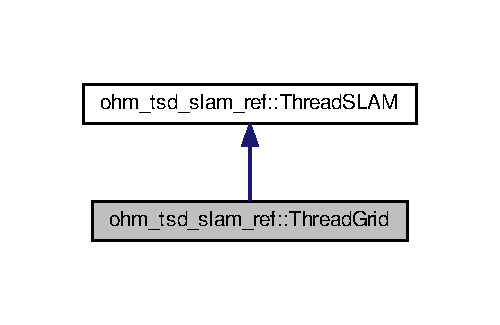
\includegraphics[width=240pt]{classohm__tsd__slam__ref_1_1ThreadGrid__inherit__graph}
\end{center}
\end{figure}


Collaboration diagram for ohm\-\_\-tsd\-\_\-slam\-\_\-ref\-:\-:Thread\-Grid\-:\nopagebreak
\begin{figure}[H]
\begin{center}
\leavevmode
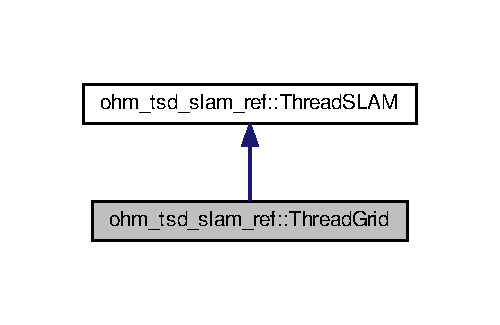
\includegraphics[width=240pt]{classohm__tsd__slam__ref_1_1ThreadGrid__coll__graph}
\end{center}
\end{figure}
\subsection*{Public Member Functions}
\begin{DoxyCompactItemize}
\item 
\hyperlink{classohm__tsd__slam__ref_1_1ThreadGrid_a23ff222ecd6e64afde2e8c926e40889c}{Thread\-Grid} (obvious\-::\-Tsd\-Grid $\ast$grid, ros\-::\-Node\-Handle $\ast$const nh, const double x\-Offset, const double y\-Offset)
\item 
virtual \hyperlink{classohm__tsd__slam__ref_1_1ThreadGrid_af82bbcec8320f6bc6fb1797f062fa8d9}{$\sim$\-Thread\-Grid} ()
\end{DoxyCompactItemize}
\subsection*{Protected Member Functions}
\begin{DoxyCompactItemize}
\item 
virtual void \hyperlink{classohm__tsd__slam__ref_1_1ThreadGrid_ab5153ffea8c253924f5d5f1f05d9aa59}{event\-Loop} (void)
\end{DoxyCompactItemize}
\subsection*{Private Member Functions}
\begin{DoxyCompactItemize}
\item 
bool \hyperlink{classohm__tsd__slam__ref_1_1ThreadGrid_a59566780b74cff54ab8a9ac398e29657}{get\-Map\-Serv\-Call\-Back} (nav\-\_\-msgs\-::\-Get\-Map\-::\-Request \&req, nav\-\_\-msgs\-::\-Get\-Map\-::\-Response \&res)
\end{DoxyCompactItemize}
\subsection*{Private Attributes}
\begin{DoxyCompactItemize}
\item 
nav\-\_\-msgs\-::\-Occupancy\-Grid $\ast$ \hyperlink{classohm__tsd__slam__ref_1_1ThreadGrid_aabac708b71745a854f552156b8aef2ae}{\-\_\-occ\-Grid}
\item 
ros\-::\-Service\-Server \hyperlink{classohm__tsd__slam__ref_1_1ThreadGrid_aa37d0527a25f70d3e6869229b6808810}{\-\_\-get\-Map\-Serv}
\item 
char $\ast$ \hyperlink{classohm__tsd__slam__ref_1_1ThreadGrid_a3e1350e3d4943ab408ae9b0935300972}{\-\_\-occ\-Grid\-Content}
\item 
double $\ast$ \hyperlink{classohm__tsd__slam__ref_1_1ThreadGrid_a01adc5e95f879fbed0686a008a44ea86}{\-\_\-grid\-Coords}
\item 
unsigned int \hyperlink{classohm__tsd__slam__ref_1_1ThreadGrid_a4e18fa3923e4a016ad2ca963ccd318d7}{\-\_\-width}
\item 
unsigned int \hyperlink{classohm__tsd__slam__ref_1_1ThreadGrid_a549634eab5110b6b3f0ce5bf5ee82fca}{\-\_\-height}
\item 
double \hyperlink{classohm__tsd__slam__ref_1_1ThreadGrid_a91bad701055d367eefe1e4b3639a71fd}{\-\_\-cell\-Size}
\item 
ros\-::\-Publisher \hyperlink{classohm__tsd__slam__ref_1_1ThreadGrid_a6a7f8db27c4cee799aaf328caacd2bdf}{\-\_\-grid\-Pub}
\item 
ros\-::\-Publisher \hyperlink{classohm__tsd__slam__ref_1_1ThreadGrid_a86ea0357d397f91ef76eb40389fb55e0}{\-\_\-pub\-Color\-Image}
\item 
bool \hyperlink{classohm__tsd__slam__ref_1_1ThreadGrid_a2b8fe225e961331b72894697f1a8b120}{\-\_\-pub\-Tsd\-Color\-Map}
\item 
unsigned int \hyperlink{classohm__tsd__slam__ref_1_1ThreadGrid_a0e9769acfadae7638005529607d7ff79}{\-\_\-obj\-Inflate\-Factor}
\item 
bool \hyperlink{classohm__tsd__slam__ref_1_1ThreadGrid_a2eef7cdb2d93710b69cd4858a7e7d337}{\-\_\-object\-Inflation}
\end{DoxyCompactItemize}
\subsection*{Additional Inherited Members}


\subsection{Detailed Description}
Class implementing a thread that generates an occupancy grid. 

\begin{DoxyAuthor}{Author}
Philipp Koch, Stefan May 
\end{DoxyAuthor}


\subsection{Constructor \& Destructor Documentation}
\hypertarget{classohm__tsd__slam__ref_1_1ThreadGrid_a23ff222ecd6e64afde2e8c926e40889c}{\index{ohm\-\_\-tsd\-\_\-slam\-\_\-ref\-::\-Thread\-Grid@{ohm\-\_\-tsd\-\_\-slam\-\_\-ref\-::\-Thread\-Grid}!Thread\-Grid@{Thread\-Grid}}
\index{Thread\-Grid@{Thread\-Grid}!ohm_tsd_slam_ref::ThreadGrid@{ohm\-\_\-tsd\-\_\-slam\-\_\-ref\-::\-Thread\-Grid}}
\subsubsection[{Thread\-Grid}]{\setlength{\rightskip}{0pt plus 5cm}ohm\-\_\-tsd\-\_\-slam\-\_\-ref\-::\-Thread\-Grid\-::\-Thread\-Grid (
\begin{DoxyParamCaption}
\item[{obvious\-::\-Tsd\-Grid $\ast$}]{grid, }
\item[{ros\-::\-Node\-Handle $\ast$const}]{nh, }
\item[{const double}]{x\-Offset, }
\item[{const double}]{y\-Offset}
\end{DoxyParamCaption}
)}}\label{classohm__tsd__slam__ref_1_1ThreadGrid_a23ff222ecd6e64afde2e8c926e40889c}
Constructor 
\begin{DoxyParams}{Parameters}
{\em grid} & Representation \\
\hline
{\em nh} & R\-O\-S nodehandle \\
\hline
{\em x\-Offset} & \\
\hline
{\em y\-Offset} & \\
\hline
\end{DoxyParams}
\begin{DoxyRefDesc}{Todo}
\item[\hyperlink{todo__todo000016}{Todo}]warum prv\-Nh ohne string template $<$$>$ \end{DoxyRefDesc}
\hypertarget{classohm__tsd__slam__ref_1_1ThreadGrid_af82bbcec8320f6bc6fb1797f062fa8d9}{\index{ohm\-\_\-tsd\-\_\-slam\-\_\-ref\-::\-Thread\-Grid@{ohm\-\_\-tsd\-\_\-slam\-\_\-ref\-::\-Thread\-Grid}!$\sim$\-Thread\-Grid@{$\sim$\-Thread\-Grid}}
\index{$\sim$\-Thread\-Grid@{$\sim$\-Thread\-Grid}!ohm_tsd_slam_ref::ThreadGrid@{ohm\-\_\-tsd\-\_\-slam\-\_\-ref\-::\-Thread\-Grid}}
\subsubsection[{$\sim$\-Thread\-Grid}]{\setlength{\rightskip}{0pt plus 5cm}ohm\-\_\-tsd\-\_\-slam\-\_\-ref\-::\-Thread\-Grid\-::$\sim$\-Thread\-Grid (
\begin{DoxyParamCaption}
{}
\end{DoxyParamCaption}
)\hspace{0.3cm}{\ttfamily [virtual]}}}\label{classohm__tsd__slam__ref_1_1ThreadGrid_af82bbcec8320f6bc6fb1797f062fa8d9}
Destructor 

\subsection{Member Function Documentation}
\hypertarget{classohm__tsd__slam__ref_1_1ThreadGrid_ab5153ffea8c253924f5d5f1f05d9aa59}{\index{ohm\-\_\-tsd\-\_\-slam\-\_\-ref\-::\-Thread\-Grid@{ohm\-\_\-tsd\-\_\-slam\-\_\-ref\-::\-Thread\-Grid}!event\-Loop@{event\-Loop}}
\index{event\-Loop@{event\-Loop}!ohm_tsd_slam_ref::ThreadGrid@{ohm\-\_\-tsd\-\_\-slam\-\_\-ref\-::\-Thread\-Grid}}
\subsubsection[{event\-Loop}]{\setlength{\rightskip}{0pt plus 5cm}void ohm\-\_\-tsd\-\_\-slam\-\_\-ref\-::\-Thread\-Grid\-::event\-Loop (
\begin{DoxyParamCaption}
\item[{void}]{}
\end{DoxyParamCaption}
)\hspace{0.3cm}{\ttfamily [protected]}, {\ttfamily [virtual]}}}\label{classohm__tsd__slam__ref_1_1ThreadGrid_ab5153ffea8c253924f5d5f1f05d9aa59}
Event Loop for thread \begin{DoxyRefDesc}{Todo}
\item[\hyperlink{todo__todo000018}{Todo}]können wir bitttttte die occupied cells berechnung mal durchgehen \end{DoxyRefDesc}
\begin{DoxyRefDesc}{Todo}
\item[\hyperlink{todo__todo000017}{Todo}]unsigned char$\ast$ color\-Buffer -\/ std\-::vector? \end{DoxyRefDesc}


Implements \hyperlink{classohm__tsd__slam__ref_1_1ThreadSLAM_a7f8eec542ea75b833d981b9c4af5beb0}{ohm\-\_\-tsd\-\_\-slam\-\_\-ref\-::\-Thread\-S\-L\-A\-M}.

\hypertarget{classohm__tsd__slam__ref_1_1ThreadGrid_a59566780b74cff54ab8a9ac398e29657}{\index{ohm\-\_\-tsd\-\_\-slam\-\_\-ref\-::\-Thread\-Grid@{ohm\-\_\-tsd\-\_\-slam\-\_\-ref\-::\-Thread\-Grid}!get\-Map\-Serv\-Call\-Back@{get\-Map\-Serv\-Call\-Back}}
\index{get\-Map\-Serv\-Call\-Back@{get\-Map\-Serv\-Call\-Back}!ohm_tsd_slam_ref::ThreadGrid@{ohm\-\_\-tsd\-\_\-slam\-\_\-ref\-::\-Thread\-Grid}}
\subsubsection[{get\-Map\-Serv\-Call\-Back}]{\setlength{\rightskip}{0pt plus 5cm}bool ohm\-\_\-tsd\-\_\-slam\-\_\-ref\-::\-Thread\-Grid\-::get\-Map\-Serv\-Call\-Back (
\begin{DoxyParamCaption}
\item[{nav\-\_\-msgs\-::\-Get\-Map\-::\-Request \&}]{req, }
\item[{nav\-\_\-msgs\-::\-Get\-Map\-::\-Response \&}]{res}
\end{DoxyParamCaption}
)\hspace{0.3cm}{\ttfamily [private]}}}\label{classohm__tsd__slam__ref_1_1ThreadGrid_a59566780b74cff54ab8a9ac398e29657}
R\-O\-S service callback method for Get\-Map service Get the map as a nav\-\_\-msgs/\-Occupancy\-Grid 
\begin{DoxyParams}{Parameters}
{\em req} & Request \\
\hline
{\em res} & Response \\
\hline
\end{DoxyParams}
\begin{DoxyReturn}{Returns}
true if successful 
\end{DoxyReturn}


\subsection{Member Data Documentation}
\hypertarget{classohm__tsd__slam__ref_1_1ThreadGrid_a91bad701055d367eefe1e4b3639a71fd}{\index{ohm\-\_\-tsd\-\_\-slam\-\_\-ref\-::\-Thread\-Grid@{ohm\-\_\-tsd\-\_\-slam\-\_\-ref\-::\-Thread\-Grid}!\-\_\-cell\-Size@{\-\_\-cell\-Size}}
\index{\-\_\-cell\-Size@{\-\_\-cell\-Size}!ohm_tsd_slam_ref::ThreadGrid@{ohm\-\_\-tsd\-\_\-slam\-\_\-ref\-::\-Thread\-Grid}}
\subsubsection[{\-\_\-cell\-Size}]{\setlength{\rightskip}{0pt plus 5cm}double ohm\-\_\-tsd\-\_\-slam\-\_\-ref\-::\-Thread\-Grid\-::\-\_\-cell\-Size\hspace{0.3cm}{\ttfamily [private]}}}\label{classohm__tsd__slam__ref_1_1ThreadGrid_a91bad701055d367eefe1e4b3639a71fd}
Grid resolution \hypertarget{classohm__tsd__slam__ref_1_1ThreadGrid_aa37d0527a25f70d3e6869229b6808810}{\index{ohm\-\_\-tsd\-\_\-slam\-\_\-ref\-::\-Thread\-Grid@{ohm\-\_\-tsd\-\_\-slam\-\_\-ref\-::\-Thread\-Grid}!\-\_\-get\-Map\-Serv@{\-\_\-get\-Map\-Serv}}
\index{\-\_\-get\-Map\-Serv@{\-\_\-get\-Map\-Serv}!ohm_tsd_slam_ref::ThreadGrid@{ohm\-\_\-tsd\-\_\-slam\-\_\-ref\-::\-Thread\-Grid}}
\subsubsection[{\-\_\-get\-Map\-Serv}]{\setlength{\rightskip}{0pt plus 5cm}ros\-::\-Service\-Server ohm\-\_\-tsd\-\_\-slam\-\_\-ref\-::\-Thread\-Grid\-::\-\_\-get\-Map\-Serv\hspace{0.3cm}{\ttfamily [private]}}}\label{classohm__tsd__slam__ref_1_1ThreadGrid_aa37d0527a25f70d3e6869229b6808810}
R\-O\-S server for Get\-Map service \hypertarget{classohm__tsd__slam__ref_1_1ThreadGrid_a01adc5e95f879fbed0686a008a44ea86}{\index{ohm\-\_\-tsd\-\_\-slam\-\_\-ref\-::\-Thread\-Grid@{ohm\-\_\-tsd\-\_\-slam\-\_\-ref\-::\-Thread\-Grid}!\-\_\-grid\-Coords@{\-\_\-grid\-Coords}}
\index{\-\_\-grid\-Coords@{\-\_\-grid\-Coords}!ohm_tsd_slam_ref::ThreadGrid@{ohm\-\_\-tsd\-\_\-slam\-\_\-ref\-::\-Thread\-Grid}}
\subsubsection[{\-\_\-grid\-Coords}]{\setlength{\rightskip}{0pt plus 5cm}double$\ast$ ohm\-\_\-tsd\-\_\-slam\-\_\-ref\-::\-Thread\-Grid\-::\-\_\-grid\-Coords\hspace{0.3cm}{\ttfamily [private]}}}\label{classohm__tsd__slam__ref_1_1ThreadGrid_a01adc5e95f879fbed0686a008a44ea86}
Buffer for grid coordinates \hypertarget{classohm__tsd__slam__ref_1_1ThreadGrid_a6a7f8db27c4cee799aaf328caacd2bdf}{\index{ohm\-\_\-tsd\-\_\-slam\-\_\-ref\-::\-Thread\-Grid@{ohm\-\_\-tsd\-\_\-slam\-\_\-ref\-::\-Thread\-Grid}!\-\_\-grid\-Pub@{\-\_\-grid\-Pub}}
\index{\-\_\-grid\-Pub@{\-\_\-grid\-Pub}!ohm_tsd_slam_ref::ThreadGrid@{ohm\-\_\-tsd\-\_\-slam\-\_\-ref\-::\-Thread\-Grid}}
\subsubsection[{\-\_\-grid\-Pub}]{\setlength{\rightskip}{0pt plus 5cm}ros\-::\-Publisher ohm\-\_\-tsd\-\_\-slam\-\_\-ref\-::\-Thread\-Grid\-::\-\_\-grid\-Pub\hspace{0.3cm}{\ttfamily [private]}}}\label{classohm__tsd__slam__ref_1_1ThreadGrid_a6a7f8db27c4cee799aaf328caacd2bdf}
R\-O\-S occupancy grid publisher \hypertarget{classohm__tsd__slam__ref_1_1ThreadGrid_a549634eab5110b6b3f0ce5bf5ee82fca}{\index{ohm\-\_\-tsd\-\_\-slam\-\_\-ref\-::\-Thread\-Grid@{ohm\-\_\-tsd\-\_\-slam\-\_\-ref\-::\-Thread\-Grid}!\-\_\-height@{\-\_\-height}}
\index{\-\_\-height@{\-\_\-height}!ohm_tsd_slam_ref::ThreadGrid@{ohm\-\_\-tsd\-\_\-slam\-\_\-ref\-::\-Thread\-Grid}}
\subsubsection[{\-\_\-height}]{\setlength{\rightskip}{0pt plus 5cm}unsigned int ohm\-\_\-tsd\-\_\-slam\-\_\-ref\-::\-Thread\-Grid\-::\-\_\-height\hspace{0.3cm}{\ttfamily [private]}}}\label{classohm__tsd__slam__ref_1_1ThreadGrid_a549634eab5110b6b3f0ce5bf5ee82fca}
Grid dimension \hypertarget{classohm__tsd__slam__ref_1_1ThreadGrid_a2eef7cdb2d93710b69cd4858a7e7d337}{\index{ohm\-\_\-tsd\-\_\-slam\-\_\-ref\-::\-Thread\-Grid@{ohm\-\_\-tsd\-\_\-slam\-\_\-ref\-::\-Thread\-Grid}!\-\_\-object\-Inflation@{\-\_\-object\-Inflation}}
\index{\-\_\-object\-Inflation@{\-\_\-object\-Inflation}!ohm_tsd_slam_ref::ThreadGrid@{ohm\-\_\-tsd\-\_\-slam\-\_\-ref\-::\-Thread\-Grid}}
\subsubsection[{\-\_\-object\-Inflation}]{\setlength{\rightskip}{0pt plus 5cm}bool ohm\-\_\-tsd\-\_\-slam\-\_\-ref\-::\-Thread\-Grid\-::\-\_\-object\-Inflation\hspace{0.3cm}{\ttfamily [private]}}}\label{classohm__tsd__slam__ref_1_1ThreadGrid_a2eef7cdb2d93710b69cd4858a7e7d337}
Object inflation control flag \hypertarget{classohm__tsd__slam__ref_1_1ThreadGrid_a0e9769acfadae7638005529607d7ff79}{\index{ohm\-\_\-tsd\-\_\-slam\-\_\-ref\-::\-Thread\-Grid@{ohm\-\_\-tsd\-\_\-slam\-\_\-ref\-::\-Thread\-Grid}!\-\_\-obj\-Inflate\-Factor@{\-\_\-obj\-Inflate\-Factor}}
\index{\-\_\-obj\-Inflate\-Factor@{\-\_\-obj\-Inflate\-Factor}!ohm_tsd_slam_ref::ThreadGrid@{ohm\-\_\-tsd\-\_\-slam\-\_\-ref\-::\-Thread\-Grid}}
\subsubsection[{\-\_\-obj\-Inflate\-Factor}]{\setlength{\rightskip}{0pt plus 5cm}unsigned int ohm\-\_\-tsd\-\_\-slam\-\_\-ref\-::\-Thread\-Grid\-::\-\_\-obj\-Inflate\-Factor\hspace{0.3cm}{\ttfamily [private]}}}\label{classohm__tsd__slam__ref_1_1ThreadGrid_a0e9769acfadae7638005529607d7ff79}
Object inflation factor \hypertarget{classohm__tsd__slam__ref_1_1ThreadGrid_aabac708b71745a854f552156b8aef2ae}{\index{ohm\-\_\-tsd\-\_\-slam\-\_\-ref\-::\-Thread\-Grid@{ohm\-\_\-tsd\-\_\-slam\-\_\-ref\-::\-Thread\-Grid}!\-\_\-occ\-Grid@{\-\_\-occ\-Grid}}
\index{\-\_\-occ\-Grid@{\-\_\-occ\-Grid}!ohm_tsd_slam_ref::ThreadGrid@{ohm\-\_\-tsd\-\_\-slam\-\_\-ref\-::\-Thread\-Grid}}
\subsubsection[{\-\_\-occ\-Grid}]{\setlength{\rightskip}{0pt plus 5cm}nav\-\_\-msgs\-::\-Occupancy\-Grid$\ast$ ohm\-\_\-tsd\-\_\-slam\-\_\-ref\-::\-Thread\-Grid\-::\-\_\-occ\-Grid\hspace{0.3cm}{\ttfamily [private]}}}\label{classohm__tsd__slam__ref_1_1ThreadGrid_aabac708b71745a854f552156b8aef2ae}
Occupancy grid \hypertarget{classohm__tsd__slam__ref_1_1ThreadGrid_a3e1350e3d4943ab408ae9b0935300972}{\index{ohm\-\_\-tsd\-\_\-slam\-\_\-ref\-::\-Thread\-Grid@{ohm\-\_\-tsd\-\_\-slam\-\_\-ref\-::\-Thread\-Grid}!\-\_\-occ\-Grid\-Content@{\-\_\-occ\-Grid\-Content}}
\index{\-\_\-occ\-Grid\-Content@{\-\_\-occ\-Grid\-Content}!ohm_tsd_slam_ref::ThreadGrid@{ohm\-\_\-tsd\-\_\-slam\-\_\-ref\-::\-Thread\-Grid}}
\subsubsection[{\-\_\-occ\-Grid\-Content}]{\setlength{\rightskip}{0pt plus 5cm}char$\ast$ ohm\-\_\-tsd\-\_\-slam\-\_\-ref\-::\-Thread\-Grid\-::\-\_\-occ\-Grid\-Content\hspace{0.3cm}{\ttfamily [private]}}}\label{classohm__tsd__slam__ref_1_1ThreadGrid_a3e1350e3d4943ab408ae9b0935300972}
Buffer for occupancy grid content \begin{DoxyRefDesc}{Todo}
\item[\hyperlink{todo__todo000019}{Todo}]eventuell abändern, veraltet \end{DoxyRefDesc}
\hypertarget{classohm__tsd__slam__ref_1_1ThreadGrid_a86ea0357d397f91ef76eb40389fb55e0}{\index{ohm\-\_\-tsd\-\_\-slam\-\_\-ref\-::\-Thread\-Grid@{ohm\-\_\-tsd\-\_\-slam\-\_\-ref\-::\-Thread\-Grid}!\-\_\-pub\-Color\-Image@{\-\_\-pub\-Color\-Image}}
\index{\-\_\-pub\-Color\-Image@{\-\_\-pub\-Color\-Image}!ohm_tsd_slam_ref::ThreadGrid@{ohm\-\_\-tsd\-\_\-slam\-\_\-ref\-::\-Thread\-Grid}}
\subsubsection[{\-\_\-pub\-Color\-Image}]{\setlength{\rightskip}{0pt plus 5cm}ros\-::\-Publisher ohm\-\_\-tsd\-\_\-slam\-\_\-ref\-::\-Thread\-Grid\-::\-\_\-pub\-Color\-Image\hspace{0.3cm}{\ttfamily [private]}}}\label{classohm__tsd__slam__ref_1_1ThreadGrid_a86ea0357d397f91ef76eb40389fb55e0}
R\-O\-S color image publisher \hypertarget{classohm__tsd__slam__ref_1_1ThreadGrid_a2b8fe225e961331b72894697f1a8b120}{\index{ohm\-\_\-tsd\-\_\-slam\-\_\-ref\-::\-Thread\-Grid@{ohm\-\_\-tsd\-\_\-slam\-\_\-ref\-::\-Thread\-Grid}!\-\_\-pub\-Tsd\-Color\-Map@{\-\_\-pub\-Tsd\-Color\-Map}}
\index{\-\_\-pub\-Tsd\-Color\-Map@{\-\_\-pub\-Tsd\-Color\-Map}!ohm_tsd_slam_ref::ThreadGrid@{ohm\-\_\-tsd\-\_\-slam\-\_\-ref\-::\-Thread\-Grid}}
\subsubsection[{\-\_\-pub\-Tsd\-Color\-Map}]{\setlength{\rightskip}{0pt plus 5cm}bool ohm\-\_\-tsd\-\_\-slam\-\_\-ref\-::\-Thread\-Grid\-::\-\_\-pub\-Tsd\-Color\-Map\hspace{0.3cm}{\ttfamily [private]}}}\label{classohm__tsd__slam__ref_1_1ThreadGrid_a2b8fe225e961331b72894697f1a8b120}
Publish color map control flag \hypertarget{classohm__tsd__slam__ref_1_1ThreadGrid_a4e18fa3923e4a016ad2ca963ccd318d7}{\index{ohm\-\_\-tsd\-\_\-slam\-\_\-ref\-::\-Thread\-Grid@{ohm\-\_\-tsd\-\_\-slam\-\_\-ref\-::\-Thread\-Grid}!\-\_\-width@{\-\_\-width}}
\index{\-\_\-width@{\-\_\-width}!ohm_tsd_slam_ref::ThreadGrid@{ohm\-\_\-tsd\-\_\-slam\-\_\-ref\-::\-Thread\-Grid}}
\subsubsection[{\-\_\-width}]{\setlength{\rightskip}{0pt plus 5cm}unsigned int ohm\-\_\-tsd\-\_\-slam\-\_\-ref\-::\-Thread\-Grid\-::\-\_\-width\hspace{0.3cm}{\ttfamily [private]}}}\label{classohm__tsd__slam__ref_1_1ThreadGrid_a4e18fa3923e4a016ad2ca963ccd318d7}
Grid dimension 

The documentation for this class was generated from the following files\-:\begin{DoxyCompactItemize}
\item 
src/\hyperlink{ThreadGrid_8h}{Thread\-Grid.\-h}\item 
src/\hyperlink{ThreadGrid_8cpp}{Thread\-Grid.\-cpp}\end{DoxyCompactItemize}

\hypertarget{classohm__tsd__slam__ref_1_1ThreadLocalize}{\section{ohm\-\_\-tsd\-\_\-slam\-\_\-ref\-:\-:Thread\-Localize Class Reference}
\label{classohm__tsd__slam__ref_1_1ThreadLocalize}\index{ohm\-\_\-tsd\-\_\-slam\-\_\-ref\-::\-Thread\-Localize@{ohm\-\_\-tsd\-\_\-slam\-\_\-ref\-::\-Thread\-Localize}}
}


{\ttfamily \#include $<$Thread\-Localize.\-h$>$}



Inheritance diagram for ohm\-\_\-tsd\-\_\-slam\-\_\-ref\-:\-:Thread\-Localize\-:\nopagebreak
\begin{figure}[H]
\begin{center}
\leavevmode
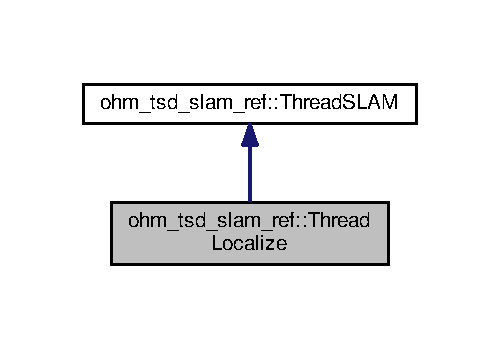
\includegraphics[width=240pt]{classohm__tsd__slam__ref_1_1ThreadLocalize__inherit__graph}
\end{center}
\end{figure}


Collaboration diagram for ohm\-\_\-tsd\-\_\-slam\-\_\-ref\-:\-:Thread\-Localize\-:\nopagebreak
\begin{figure}[H]
\begin{center}
\leavevmode
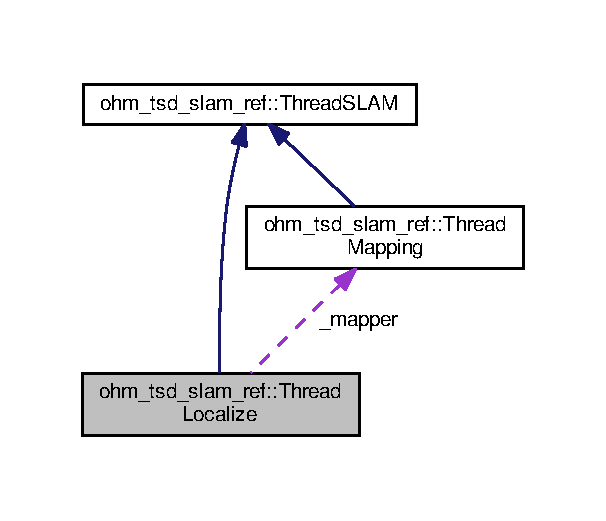
\includegraphics[width=291pt]{classohm__tsd__slam__ref_1_1ThreadLocalize__coll__graph}
\end{center}
\end{figure}
\subsection*{Public Member Functions}
\begin{DoxyCompactItemize}
\item 
\hyperlink{classohm__tsd__slam__ref_1_1ThreadLocalize_a6664fba91fb551b13cf721638b55f36e}{Thread\-Localize} (obvious\-::\-Tsd\-Grid $\ast$grid, \hyperlink{classohm__tsd__slam__ref_1_1ThreadMapping}{Thread\-Mapping} $\ast$mapper, ros\-::\-Node\-Handle $\ast$nh, std\-::string name\-Space, const double x\-Offset, const double y\-Offset)
\item 
virtual \hyperlink{classohm__tsd__slam__ref_1_1ThreadLocalize_a4cb409859b390b9b1082b8a56d760f5f}{$\sim$\-Thread\-Localize} ()
\item 
void \hyperlink{classohm__tsd__slam__ref_1_1ThreadLocalize_ab93dfc8a688c178b641ef5deec94bf91}{laser\-Call\-Back} (const sensor\-\_\-msgs\-::\-Laser\-Scan \&scan)
\end{DoxyCompactItemize}
\subsection*{Protected Member Functions}
\begin{DoxyCompactItemize}
\item 
virtual void \hyperlink{classohm__tsd__slam__ref_1_1ThreadLocalize_a93b32600effe05fe0db9fdf74cd40aa7}{event\-Loop} (void)
\end{DoxyCompactItemize}
\subsection*{Private Types}
\begin{DoxyCompactItemize}
\item 
enum \hyperlink{classohm__tsd__slam__ref_1_1ThreadLocalize_ac5ed59506607265dc4c38a64cf36156f}{Enum\-Reg\-Modes} \{ \hyperlink{classohm__tsd__slam__ref_1_1ThreadLocalize_ac5ed59506607265dc4c38a64cf36156fa4c2ccd40e418593ae90c9844a7e8b27b}{I\-C\-P} = 0, 
\hyperlink{classohm__tsd__slam__ref_1_1ThreadLocalize_ac5ed59506607265dc4c38a64cf36156faa5d6bcb6b063925c8ceee9660ba6fe82}{E\-X\-P} = 1, 
\hyperlink{classohm__tsd__slam__ref_1_1ThreadLocalize_ac5ed59506607265dc4c38a64cf36156fa5fca603cf985a7804238323fc6261c45}{P\-D\-F} = 2, 
\hyperlink{classohm__tsd__slam__ref_1_1ThreadLocalize_ac5ed59506607265dc4c38a64cf36156fae6fb70bc18328170438ececea919a178}{T\-S\-D} = 3
 \}
\end{DoxyCompactItemize}
\subsection*{Private Member Functions}
\begin{DoxyCompactItemize}
\item 
void \hyperlink{classohm__tsd__slam__ref_1_1ThreadLocalize_aec7ad646c46fd6809d7606d02388d26f}{init} (const sensor\-\_\-msgs\-::\-Laser\-Scan \&scan)
\item 
double \hyperlink{classohm__tsd__slam__ref_1_1ThreadLocalize_a2f2f07578bdc28b9d217f79b8d37e2b6}{calc\-Angle} (obvious\-::\-Matrix $\ast$T)
\item 
bool \hyperlink{classohm__tsd__slam__ref_1_1ThreadLocalize_a42b20cc96002fb42347aa292a8321589}{is\-Pose\-Change\-Significant} (obvious\-::\-Matrix $\ast$last\-Pose, obvious\-::\-Matrix $\ast$cur\-Pose)
\item 
obvious\-::\-Matrix \hyperlink{classohm__tsd__slam__ref_1_1ThreadLocalize_a0b89c7cf90db8719b2324cce13b43e5b}{do\-Registration} (obvious\-::\-Sensor\-Polar2\-D $\ast$sensor, obvious\-::\-Matrix $\ast$M, obvious\-::\-Matrix $\ast$Mvalid, obvious\-::\-Matrix $\ast$N, obvious\-::\-Matrix $\ast$Nvalid, obvious\-::\-Matrix $\ast$S, obvious\-::\-Matrix $\ast$Svalid)
\item 
bool \hyperlink{classohm__tsd__slam__ref_1_1ThreadLocalize_a9b03610d7b3f56c24c733e2cc1f922bc}{is\-Registration\-Error} (obvious\-::\-Matrix $\ast$T, const double trns\-Max, const double rot\-Max)
\item 
void \hyperlink{classohm__tsd__slam__ref_1_1ThreadLocalize_a7e09fab6884bb9752525a5b9a3223f48}{send\-Transform} (obvious\-::\-Matrix $\ast$T)
\item 
void \hyperlink{classohm__tsd__slam__ref_1_1ThreadLocalize_a3b98400814080c99c6cf5d6513b85b8d}{send\-Nan\-Transform} ()
\item 
obvious\-::\-Matrix \hyperlink{classohm__tsd__slam__ref_1_1ThreadLocalize_a8b5b655705c1c06398b725d37815084b}{mask\-Matrix} (obvious\-::\-Matrix $\ast$Mat, bool $\ast$mask, unsigned int mask\-Size, unsigned int valid\-Points)
\item 
void \hyperlink{classohm__tsd__slam__ref_1_1ThreadLocalize_a9ebe616b6e1af232d3663ea7ba8af19e}{reduce\-Resolution} (bool $\ast$const mask\-In, obvious\-::\-Matrix $\ast$mat\-In, bool $\ast$const mask\-Out, obvious\-::\-Matrix $\ast$mat\-Out, unsigned int points\-In, unsigned int points\-Out, unsigned int reduction\-Factor)
\item 
tf\-::\-Transform \hyperlink{classohm__tsd__slam__ref_1_1ThreadLocalize_acc11e43687732ffe8c81dfbeb293a6bc}{obviously\-Matrix3x3\-To\-Tf} (obvious\-::\-Matrix \&ob)
\item 
obvious\-::\-Matrix \hyperlink{classohm__tsd__slam__ref_1_1ThreadLocalize_aad3131cd2ef3eb0de3e79ed0d58a4190}{tf\-To\-Obviously\-Matrix3x3} (const tf\-::\-Transform \&tf)
\end{DoxyCompactItemize}
\subsection*{Private Attributes}
\begin{DoxyCompactItemize}
\item 
ros\-::\-Node\-Handle $\ast$ \hyperlink{classohm__tsd__slam__ref_1_1ThreadLocalize_a339ec43d3843e2049120afd424a636f7}{\-\_\-nh}
\item 
\hyperlink{classohm__tsd__slam__ref_1_1ThreadMapping}{Thread\-Mapping} \& \hyperlink{classohm__tsd__slam__ref_1_1ThreadLocalize_a73a2ed65f92fbf13e82e7b00e8354c13}{\-\_\-mapper}
\item 
obvious\-::\-Sensor\-Polar2\-D $\ast$ \hyperlink{classohm__tsd__slam__ref_1_1ThreadLocalize_ad08189f4b2c11aa3f2d75384d89088f8}{\-\_\-sensor}
\item 
bool \hyperlink{classohm__tsd__slam__ref_1_1ThreadLocalize_a936d63f4a95f0102070be527a2636f8f}{\-\_\-initialized}
\item 
const double \hyperlink{classohm__tsd__slam__ref_1_1ThreadLocalize_a09c5ac4604a298725984646e683aa600}{\-\_\-grid\-Width}
\item 
const double \hyperlink{classohm__tsd__slam__ref_1_1ThreadLocalize_af9493e2cbbce37f693bbe632374d0d2a}{\-\_\-grid\-Height}
\item 
const double \hyperlink{classohm__tsd__slam__ref_1_1ThreadLocalize_a74254a193f989fd948778e780a340b9c}{\-\_\-grid\-Off\-Set\-X}
\item 
const double \hyperlink{classohm__tsd__slam__ref_1_1ThreadLocalize_ab12390e3a1727f9d1c47fc96747bd96c}{\-\_\-grid\-Off\-Set\-Y}
\item 
const double \hyperlink{classohm__tsd__slam__ref_1_1ThreadLocalize_a2bfa898645a8b505fbc317829da277cf}{\-\_\-x\-Offset}
\item 
const double \hyperlink{classohm__tsd__slam__ref_1_1ThreadLocalize_afd9255f70ea924f91b0e628d20245803}{\-\_\-y\-Offset}
\item 
std\-::string \hyperlink{classohm__tsd__slam__ref_1_1ThreadLocalize_ae67e48692aef6eadb8a12c2c89362c94}{\-\_\-name\-Space}
\item 
ros\-::\-Time \hyperlink{classohm__tsd__slam__ref_1_1ThreadLocalize_acf1975963191b84dd1fda914a4cc15ae}{\-\_\-stamp\-Laser}
\item 
Odometry\-Analyzer $\ast$ \hyperlink{classohm__tsd__slam__ref_1_1ThreadLocalize_a719b8e1a97ec5ba8e859f24b416699a0}{\-\_\-odom\-Analyzer}
\item 
boost\-::mutex \hyperlink{classohm__tsd__slam__ref_1_1ThreadLocalize_ad1b612e37ab54ffe1958cac7d5f9c89c}{\-\_\-data\-Mutex}
\item 
double \hyperlink{classohm__tsd__slam__ref_1_1ThreadLocalize_a943d9246b84ff11c2c01f7af1a3730f9}{\-\_\-trns\-Max}
\item 
double \hyperlink{classohm__tsd__slam__ref_1_1ThreadLocalize_a59316ea269ecac73e614061fa3f618df}{\-\_\-trns\-Velocity\-Max}
\item 
double \hyperlink{classohm__tsd__slam__ref_1_1ThreadLocalize_a4eec8ac0c4da6cc90fe5dcc22cee2447}{\-\_\-rot\-Max}
\item 
double \hyperlink{classohm__tsd__slam__ref_1_1ThreadLocalize_ab72a7278c4ce34dab852571b7c83705c}{\-\_\-rot\-Velocity\-Max}
\item 
\hyperlink{classohm__tsd__slam__ref_1_1ThreadLocalize_ac5ed59506607265dc4c38a64cf36156f}{Enum\-Reg\-Modes} \hyperlink{classohm__tsd__slam__ref_1_1ThreadLocalize_ace3a4195d80299e3eb37be6c3a06a218}{\-\_\-reg\-Mode}
\item 
unsigned int \hyperlink{classohm__tsd__slam__ref_1_1ThreadLocalize_a756d269b7f0782d3e789f29bfc7d838d}{\-\_\-ran\-Trials}
\item 
double \hyperlink{classohm__tsd__slam__ref_1_1ThreadLocalize_a2e9f4af9a78a5c16b1a4966b1e28a27b}{\-\_\-ran\-Eps\-Thresh}
\item 
unsigned int \hyperlink{classohm__tsd__slam__ref_1_1ThreadLocalize_a33d533907a160e94d357ecd3d8226f9b}{\-\_\-ran\-Size\-Ctrl\-Set}
\item 
double \hyperlink{classohm__tsd__slam__ref_1_1ThreadLocalize_a5ab8f03d41a726e561c95be6d6f090a7}{\-\_\-ran\-Phi\-Max}
\item 
std\-::deque\\*
$<$ sensor\-\_\-msgs\-::\-Laser\-Scan $\ast$ $>$ \hyperlink{classohm__tsd__slam__ref_1_1ThreadLocalize_ab4560c87e6163708f39d4cdfc2f8a074}{\-\_\-laser\-Data}
\item 
double $\ast$ \hyperlink{classohm__tsd__slam__ref_1_1ThreadLocalize_a3339b24a6b047266ceda1c160c79b1de}{\-\_\-model\-Coords}
\item 
double $\ast$ \hyperlink{classohm__tsd__slam__ref_1_1ThreadLocalize_ab787c1c72a9d4ac14e08c05519530e63}{\-\_\-model\-Normals}
\item 
bool $\ast$ \hyperlink{classohm__tsd__slam__ref_1_1ThreadLocalize_a00672731c254282c9e469636245b49ba}{\-\_\-mask\-M}
\item 
double $\ast$ \hyperlink{classohm__tsd__slam__ref_1_1ThreadLocalize_a44d298a710aa05043423e8894e8454a0}{\-\_\-scene}
\item 
bool $\ast$ \hyperlink{classohm__tsd__slam__ref_1_1ThreadLocalize_a0f697cbf384346d1c13504830a83d768}{\-\_\-mask\-S}
\item 
obvious\-::\-Ray\-Cast\-Polar2\-D $\ast$ \hyperlink{classohm__tsd__slam__ref_1_1ThreadLocalize_acf45081cf4d42221dbc924b9fd6a1384}{\-\_\-ray\-Caster}
\item 
obvious\-::\-Pair\-Assignment $\ast$ \hyperlink{classohm__tsd__slam__ref_1_1ThreadLocalize_a45c7b109a3a9f22e0c60111c58eb0dd3}{\-\_\-assigner}
\item 
obvious\-::\-Out\-Of\-Bounds\-Filter2\-D $\ast$ \hyperlink{classohm__tsd__slam__ref_1_1ThreadLocalize_aac86a10eecf70da80d5198e9296e2aea}{\-\_\-filter\-Bounds}
\item 
obvious\-::\-Distance\-Filter $\ast$ \hyperlink{classohm__tsd__slam__ref_1_1ThreadLocalize_a34e17bd9ddbcf1431feb2cca272d8d69}{\-\_\-filter\-Dist}
\item 
obvious\-::\-Reciprocal\-Filter $\ast$ \hyperlink{classohm__tsd__slam__ref_1_1ThreadLocalize_a4444f42e17414907a35919adc4904268}{\-\_\-filter\-Reciprocal}
\item 
obvious\-::\-I\-Rigid\-Estimator $\ast$ \hyperlink{classohm__tsd__slam__ref_1_1ThreadLocalize_a34dc7fcb1cc798542270309014f09b93}{\-\_\-estimator}
\item 
obvious\-::\-Icp $\ast$ \hyperlink{classohm__tsd__slam__ref_1_1ThreadLocalize_a03e76d4fd6e599eb2e508dde1553c278}{\-\_\-icp}
\item 
obvious\-::\-Random\-Normal\-Matching $\ast$ \hyperlink{classohm__tsd__slam__ref_1_1ThreadLocalize_a527f8668ebe51a6bc7cadba7075c8c3f}{\-\_\-\-Random\-Normal\-Matcher}
\item 
obvious\-::\-P\-D\-F\-Matching $\ast$ \hyperlink{classohm__tsd__slam__ref_1_1ThreadLocalize_ad9d5e74c4f7b20dcb89e108ad8cfbe08}{\-\_\-\-P\-D\-F\-Matcher}
\item 
obvious\-::\-T\-S\-D\-\_\-\-P\-D\-F\-Matching $\ast$ \hyperlink{classohm__tsd__slam__ref_1_1ThreadLocalize_a8c7ca5e711fc2a346d130c9074b4f14d}{\-\_\-\-T\-S\-D\-\_\-\-P\-D\-F\-Matcher}
\item 
obvious\-::\-Matrix $\ast$ \hyperlink{classohm__tsd__slam__ref_1_1ThreadLocalize_a9b1c9b9fbbf202c5532755553cb42964}{\-\_\-last\-Pose}
\item 
ros\-::\-Publisher \hyperlink{classohm__tsd__slam__ref_1_1ThreadLocalize_a4072511df787f573ce74945a3021cd70}{\-\_\-pose\-Pub}
\item 
geometry\-\_\-msgs\-::\-Pose\-Stamped \hyperlink{classohm__tsd__slam__ref_1_1ThreadLocalize_a53b8418b5cb138095c170ee523c5e433}{\-\_\-pose\-Stamped}
\item 
tf\-::\-Transform\-Broadcaster \hyperlink{classohm__tsd__slam__ref_1_1ThreadLocalize_a422982c64baaa0ea6b2e259c78bb14f8}{\-\_\-tf\-Broadcaster}
\item 
tf\-::\-Transform\-Listener \hyperlink{classohm__tsd__slam__ref_1_1ThreadLocalize_a224fab0e74f4e79a3bd7477c7ba67927}{\-\_\-tf\-Listener}
\item 
tf\-::\-Stamped\-Transform \hyperlink{classohm__tsd__slam__ref_1_1ThreadLocalize_ad6eb4ec2cbb72976a751195aaa87b230}{\-\_\-tf\-Reader}
\item 
tf\-::\-Stamped\-Transform \hyperlink{classohm__tsd__slam__ref_1_1ThreadLocalize_a58c3e63ca51b4f667361138ca9612a43}{\-\_\-tf}
\item 
tf\-::\-Transform \hyperlink{classohm__tsd__slam__ref_1_1ThreadLocalize_a865325fdc2badfde0512622d52d60f46}{\-\_\-tf\-Laser}
\item 
std\-::string \hyperlink{classohm__tsd__slam__ref_1_1ThreadLocalize_a49f36ec368f39a906125435adb7fa231}{\-\_\-tf\-Footprint\-Frame\-Id}
\item 
std\-::string \hyperlink{classohm__tsd__slam__ref_1_1ThreadLocalize_a4f3c79f1893a406885983bd8984954e2}{\-\_\-tf\-Odom\-Frame\-Id}
\item 
std\-::string \hyperlink{classohm__tsd__slam__ref_1_1ThreadLocalize_ab83a495abfe38788855cd283334052ee}{\-\_\-tf\-Base\-Frame\-Id}
\item 
std\-::string \hyperlink{classohm__tsd__slam__ref_1_1ThreadLocalize_a15312866770a11e59f0e2e260a5d8c05}{\-\_\-tf\-Child\-Frame\-Id}
\item 
bool \hyperlink{classohm__tsd__slam__ref_1_1ThreadLocalize_a50a25580c50a3b14d04a548416142d6c}{\-\_\-use\-Odom\-Rescue}
\item 
bool \hyperlink{classohm__tsd__slam__ref_1_1ThreadLocalize_a60894678d5815e42124c78eef219cf8b}{\-\_\-odom\-Tf\-Is\-Valid}
\item 
ros\-::\-Duration \hyperlink{classohm__tsd__slam__ref_1_1ThreadLocalize_a5f43425ab2bb540e72205ef83e37d4ff}{\-\_\-wait\-For\-Odom\-Tf}
\item 
ros\-::\-Time \hyperlink{classohm__tsd__slam__ref_1_1ThreadLocalize_a3993fb6424dd9af667ddf0b14cdf2fe4}{\-\_\-stamp\-Laser\-Old}
\item 
bool \hyperlink{classohm__tsd__slam__ref_1_1ThreadLocalize_a176899f67fbf706a756853a8af968fd5}{\-\_\-reverse\-Scan}
\item 
double \hyperlink{classohm__tsd__slam__ref_1_1ThreadLocalize_a6170ca0dd6108536689c4dab3f7425f6}{\-\_\-las\-Min\-Range}
\end{DoxyCompactItemize}
\subsection*{Additional Inherited Members}


\subsection{Member Enumeration Documentation}
\hypertarget{classohm__tsd__slam__ref_1_1ThreadLocalize_ac5ed59506607265dc4c38a64cf36156f}{\index{ohm\-\_\-tsd\-\_\-slam\-\_\-ref\-::\-Thread\-Localize@{ohm\-\_\-tsd\-\_\-slam\-\_\-ref\-::\-Thread\-Localize}!Enum\-Reg\-Modes@{Enum\-Reg\-Modes}}
\index{Enum\-Reg\-Modes@{Enum\-Reg\-Modes}!ohm_tsd_slam_ref::ThreadLocalize@{ohm\-\_\-tsd\-\_\-slam\-\_\-ref\-::\-Thread\-Localize}}
\subsubsection[{Enum\-Reg\-Modes}]{\setlength{\rightskip}{0pt plus 5cm}enum {\bf ohm\-\_\-tsd\-\_\-slam\-\_\-ref\-::\-Thread\-Localize\-::\-Enum\-Reg\-Modes}\hspace{0.3cm}{\ttfamily [private]}}}\label{classohm__tsd__slam__ref_1_1ThreadLocalize_ac5ed59506607265dc4c38a64cf36156f}
\begin{Desc}
\item[Enumerator]\par
\begin{description}
\index{I\-C\-P@{I\-C\-P}!ohm\-\_\-tsd\-\_\-slam\-\_\-ref\-::\-Thread\-Localize@{ohm\-\_\-tsd\-\_\-slam\-\_\-ref\-::\-Thread\-Localize}}\index{ohm\-\_\-tsd\-\_\-slam\-\_\-ref\-::\-Thread\-Localize@{ohm\-\_\-tsd\-\_\-slam\-\_\-ref\-::\-Thread\-Localize}!I\-C\-P@{I\-C\-P}}\item[{\em 
\hypertarget{classohm__tsd__slam__ref_1_1ThreadLocalize_ac5ed59506607265dc4c38a64cf36156fa4c2ccd40e418593ae90c9844a7e8b27b}{I\-C\-P}\label{classohm__tsd__slam__ref_1_1ThreadLocalize_ac5ed59506607265dc4c38a64cf36156fa4c2ccd40e418593ae90c9844a7e8b27b}
}]Registration with I\-C\-P only. \index{E\-X\-P@{E\-X\-P}!ohm\-\_\-tsd\-\_\-slam\-\_\-ref\-::\-Thread\-Localize@{ohm\-\_\-tsd\-\_\-slam\-\_\-ref\-::\-Thread\-Localize}}\index{ohm\-\_\-tsd\-\_\-slam\-\_\-ref\-::\-Thread\-Localize@{ohm\-\_\-tsd\-\_\-slam\-\_\-ref\-::\-Thread\-Localize}!E\-X\-P@{E\-X\-P}}\item[{\em 
\hypertarget{classohm__tsd__slam__ref_1_1ThreadLocalize_ac5ed59506607265dc4c38a64cf36156faa5d6bcb6b063925c8ceee9660ba6fe82}{E\-X\-P}\label{classohm__tsd__slam__ref_1_1ThreadLocalize_ac5ed59506607265dc4c38a64cf36156faa5d6bcb6b063925c8ceee9660ba6fe82}
}]\index{P\-D\-F@{P\-D\-F}!ohm\-\_\-tsd\-\_\-slam\-\_\-ref\-::\-Thread\-Localize@{ohm\-\_\-tsd\-\_\-slam\-\_\-ref\-::\-Thread\-Localize}}\index{ohm\-\_\-tsd\-\_\-slam\-\_\-ref\-::\-Thread\-Localize@{ohm\-\_\-tsd\-\_\-slam\-\_\-ref\-::\-Thread\-Localize}!P\-D\-F@{P\-D\-F}}\item[{\em 
\hypertarget{classohm__tsd__slam__ref_1_1ThreadLocalize_ac5ed59506607265dc4c38a64cf36156fa5fca603cf985a7804238323fc6261c45}{P\-D\-F}\label{classohm__tsd__slam__ref_1_1ThreadLocalize_ac5ed59506607265dc4c38a64cf36156fa5fca603cf985a7804238323fc6261c45}
}]\index{T\-S\-D@{T\-S\-D}!ohm\-\_\-tsd\-\_\-slam\-\_\-ref\-::\-Thread\-Localize@{ohm\-\_\-tsd\-\_\-slam\-\_\-ref\-::\-Thread\-Localize}}\index{ohm\-\_\-tsd\-\_\-slam\-\_\-ref\-::\-Thread\-Localize@{ohm\-\_\-tsd\-\_\-slam\-\_\-ref\-::\-Thread\-Localize}!T\-S\-D@{T\-S\-D}}\item[{\em 
\hypertarget{classohm__tsd__slam__ref_1_1ThreadLocalize_ac5ed59506607265dc4c38a64cf36156fae6fb70bc18328170438ececea919a178}{T\-S\-D}\label{classohm__tsd__slam__ref_1_1ThreadLocalize_ac5ed59506607265dc4c38a64cf36156fae6fb70bc18328170438ececea919a178}
}]\end{description}
\end{Desc}


\subsection{Constructor \& Destructor Documentation}
\hypertarget{classohm__tsd__slam__ref_1_1ThreadLocalize_a6664fba91fb551b13cf721638b55f36e}{\index{ohm\-\_\-tsd\-\_\-slam\-\_\-ref\-::\-Thread\-Localize@{ohm\-\_\-tsd\-\_\-slam\-\_\-ref\-::\-Thread\-Localize}!Thread\-Localize@{Thread\-Localize}}
\index{Thread\-Localize@{Thread\-Localize}!ohm_tsd_slam_ref::ThreadLocalize@{ohm\-\_\-tsd\-\_\-slam\-\_\-ref\-::\-Thread\-Localize}}
\subsubsection[{Thread\-Localize}]{\setlength{\rightskip}{0pt plus 5cm}ohm\-\_\-tsd\-\_\-slam\-\_\-ref\-::\-Thread\-Localize\-::\-Thread\-Localize (
\begin{DoxyParamCaption}
\item[{obvious\-::\-Tsd\-Grid $\ast$}]{grid, }
\item[{{\bf Thread\-Mapping} $\ast$}]{mapper, }
\item[{ros\-::\-Node\-Handle $\ast$}]{nh, }
\item[{std\-::string}]{name\-Space, }
\item[{const double}]{x\-Offset, }
\item[{const double}]{y\-Offset}
\end{DoxyParamCaption}
)}}\label{classohm__tsd__slam__ref_1_1ThreadLocalize_a6664fba91fb551b13cf721638b55f36e}
Constructor 
\begin{DoxyParams}{Parameters}
{\em grid} & Pointer to representation \\
\hline
{\em mapper} & Pointer to mapping thread instance \\
\hline
{\em nh} & pointer to main node handle \\
\hline
{\em name\-Space} & Namespace of this localization thread \\
\hline
{\em x\-Offset} & Origin x position \\
\hline
{\em y\-Offset} & Origin y position \\
\hline
\end{DoxyParams}
\hypertarget{classohm__tsd__slam__ref_1_1ThreadLocalize_a4cb409859b390b9b1082b8a56d760f5f}{\index{ohm\-\_\-tsd\-\_\-slam\-\_\-ref\-::\-Thread\-Localize@{ohm\-\_\-tsd\-\_\-slam\-\_\-ref\-::\-Thread\-Localize}!$\sim$\-Thread\-Localize@{$\sim$\-Thread\-Localize}}
\index{$\sim$\-Thread\-Localize@{$\sim$\-Thread\-Localize}!ohm_tsd_slam_ref::ThreadLocalize@{ohm\-\_\-tsd\-\_\-slam\-\_\-ref\-::\-Thread\-Localize}}
\subsubsection[{$\sim$\-Thread\-Localize}]{\setlength{\rightskip}{0pt plus 5cm}virtual ohm\-\_\-tsd\-\_\-slam\-\_\-ref\-::\-Thread\-Localize\-::$\sim$\-Thread\-Localize (
\begin{DoxyParamCaption}
{}
\end{DoxyParamCaption}
)\hspace{0.3cm}{\ttfamily [virtual]}}}\label{classohm__tsd__slam__ref_1_1ThreadLocalize_a4cb409859b390b9b1082b8a56d760f5f}
Destructor 

\subsection{Member Function Documentation}
\hypertarget{classohm__tsd__slam__ref_1_1ThreadLocalize_a2f2f07578bdc28b9d217f79b8d37e2b6}{\index{ohm\-\_\-tsd\-\_\-slam\-\_\-ref\-::\-Thread\-Localize@{ohm\-\_\-tsd\-\_\-slam\-\_\-ref\-::\-Thread\-Localize}!calc\-Angle@{calc\-Angle}}
\index{calc\-Angle@{calc\-Angle}!ohm_tsd_slam_ref::ThreadLocalize@{ohm\-\_\-tsd\-\_\-slam\-\_\-ref\-::\-Thread\-Localize}}
\subsubsection[{calc\-Angle}]{\setlength{\rightskip}{0pt plus 5cm}double ohm\-\_\-tsd\-\_\-slam\-\_\-ref\-::\-Thread\-Localize\-::calc\-Angle (
\begin{DoxyParamCaption}
\item[{obvious\-::\-Matrix $\ast$}]{T}
\end{DoxyParamCaption}
)\hspace{0.3cm}{\ttfamily [private]}}}\label{classohm__tsd__slam__ref_1_1ThreadLocalize_a2f2f07578bdc28b9d217f79b8d37e2b6}
Method to analyze 2\-D transformation matrix. 
\begin{DoxyParams}{Parameters}
{\em T} & Pointer to transformation matrix \\
\hline
\end{DoxyParams}
\begin{DoxyReturn}{Returns}
Calculated angle 
\end{DoxyReturn}
\hypertarget{classohm__tsd__slam__ref_1_1ThreadLocalize_a0b89c7cf90db8719b2324cce13b43e5b}{\index{ohm\-\_\-tsd\-\_\-slam\-\_\-ref\-::\-Thread\-Localize@{ohm\-\_\-tsd\-\_\-slam\-\_\-ref\-::\-Thread\-Localize}!do\-Registration@{do\-Registration}}
\index{do\-Registration@{do\-Registration}!ohm_tsd_slam_ref::ThreadLocalize@{ohm\-\_\-tsd\-\_\-slam\-\_\-ref\-::\-Thread\-Localize}}
\subsubsection[{do\-Registration}]{\setlength{\rightskip}{0pt plus 5cm}obvious\-::\-Matrix ohm\-\_\-tsd\-\_\-slam\-\_\-ref\-::\-Thread\-Localize\-::do\-Registration (
\begin{DoxyParamCaption}
\item[{obvious\-::\-Sensor\-Polar2\-D $\ast$}]{sensor, }
\item[{obvious\-::\-Matrix $\ast$}]{M, }
\item[{obvious\-::\-Matrix $\ast$}]{Mvalid, }
\item[{obvious\-::\-Matrix $\ast$}]{N, }
\item[{obvious\-::\-Matrix $\ast$}]{Nvalid, }
\item[{obvious\-::\-Matrix $\ast$}]{S, }
\item[{obvious\-::\-Matrix $\ast$}]{Svalid}
\end{DoxyParamCaption}
)\hspace{0.3cm}{\ttfamily [private]}}}\label{classohm__tsd__slam__ref_1_1ThreadLocalize_a0b89c7cf90db8719b2324cce13b43e5b}
Main registration method. Aligns two laser scans and calculates the referring 2\-D transformation matrix. 
\begin{DoxyParams}{Parameters}
{\em sensor} & Laser data container \\
\hline
{\em M} & Pointer to model points \\
\hline
{\em Mvalid} & Pointer to model points \\
\hline
{\em N} & Pointer to normals of the model \\
\hline
{\em Nvalid} & Pointer to normals of the model \\
\hline
{\em S} & Pointer to scene points \\
\hline
{\em Svalid} & Pointer to scene points \\
\hline
\end{DoxyParams}
\begin{DoxyReturn}{Returns}
2\-D transformation matrix of type obvious\-::\-Matrix 
\end{DoxyReturn}
\hypertarget{classohm__tsd__slam__ref_1_1ThreadLocalize_a93b32600effe05fe0db9fdf74cd40aa7}{\index{ohm\-\_\-tsd\-\_\-slam\-\_\-ref\-::\-Thread\-Localize@{ohm\-\_\-tsd\-\_\-slam\-\_\-ref\-::\-Thread\-Localize}!event\-Loop@{event\-Loop}}
\index{event\-Loop@{event\-Loop}!ohm_tsd_slam_ref::ThreadLocalize@{ohm\-\_\-tsd\-\_\-slam\-\_\-ref\-::\-Thread\-Localize}}
\subsubsection[{event\-Loop}]{\setlength{\rightskip}{0pt plus 5cm}virtual void ohm\-\_\-tsd\-\_\-slam\-\_\-ref\-::\-Thread\-Localize\-::event\-Loop (
\begin{DoxyParamCaption}
\item[{void}]{}
\end{DoxyParamCaption}
)\hspace{0.3cm}{\ttfamily [protected]}, {\ttfamily [virtual]}}}\label{classohm__tsd__slam__ref_1_1ThreadLocalize_a93b32600effe05fe0db9fdf74cd40aa7}
Abstract function derived from base class \hyperlink{classohm__tsd__slam__ref_1_1ThreadSLAM}{Thread\-S\-L\-A\-M}. Consists of a loop the thread never leaves until a termination call occurs. 

Implements \hyperlink{classohm__tsd__slam__ref_1_1ThreadSLAM_a7f8eec542ea75b833d981b9c4af5beb0}{ohm\-\_\-tsd\-\_\-slam\-\_\-ref\-::\-Thread\-S\-L\-A\-M}.

\hypertarget{classohm__tsd__slam__ref_1_1ThreadLocalize_aec7ad646c46fd6809d7606d02388d26f}{\index{ohm\-\_\-tsd\-\_\-slam\-\_\-ref\-::\-Thread\-Localize@{ohm\-\_\-tsd\-\_\-slam\-\_\-ref\-::\-Thread\-Localize}!init@{init}}
\index{init@{init}!ohm_tsd_slam_ref::ThreadLocalize@{ohm\-\_\-tsd\-\_\-slam\-\_\-ref\-::\-Thread\-Localize}}
\subsubsection[{init}]{\setlength{\rightskip}{0pt plus 5cm}void ohm\-\_\-tsd\-\_\-slam\-\_\-ref\-::\-Thread\-Localize\-::init (
\begin{DoxyParamCaption}
\item[{const sensor\-\_\-msgs\-::\-Laser\-Scan \&}]{scan}
\end{DoxyParamCaption}
)\hspace{0.3cm}{\ttfamily [private]}}}\label{classohm__tsd__slam__ref_1_1ThreadLocalize_aec7ad646c46fd6809d7606d02388d26f}
Init function automatically called by first received laser data. 
\begin{DoxyParams}{Parameters}
{\em scan} & Initial scan used to initialize all parameters of the thread \\
\hline
\end{DoxyParams}
\hypertarget{classohm__tsd__slam__ref_1_1ThreadLocalize_a42b20cc96002fb42347aa292a8321589}{\index{ohm\-\_\-tsd\-\_\-slam\-\_\-ref\-::\-Thread\-Localize@{ohm\-\_\-tsd\-\_\-slam\-\_\-ref\-::\-Thread\-Localize}!is\-Pose\-Change\-Significant@{is\-Pose\-Change\-Significant}}
\index{is\-Pose\-Change\-Significant@{is\-Pose\-Change\-Significant}!ohm_tsd_slam_ref::ThreadLocalize@{ohm\-\_\-tsd\-\_\-slam\-\_\-ref\-::\-Thread\-Localize}}
\subsubsection[{is\-Pose\-Change\-Significant}]{\setlength{\rightskip}{0pt plus 5cm}bool ohm\-\_\-tsd\-\_\-slam\-\_\-ref\-::\-Thread\-Localize\-::is\-Pose\-Change\-Significant (
\begin{DoxyParamCaption}
\item[{obvious\-::\-Matrix $\ast$}]{last\-Pose, }
\item[{obvious\-::\-Matrix $\ast$}]{cur\-Pose}
\end{DoxyParamCaption}
)\hspace{0.3cm}{\ttfamily [private]}}}\label{classohm__tsd__slam__ref_1_1ThreadLocalize_a42b20cc96002fb42347aa292a8321589}
Method to determine whether the localized sensor has been moved significantly (value higher than thresh). A map update is only initiated in case this method returns true. 
\begin{DoxyParams}{Parameters}
{\em last\-Pose} & Pointer to last known pose \\
\hline
{\em cur\-Pose} & Pointer to current pose \\
\hline
\end{DoxyParams}
\begin{DoxyReturn}{Returns}
True in case of significant pose change 
\end{DoxyReturn}
\hypertarget{classohm__tsd__slam__ref_1_1ThreadLocalize_a9b03610d7b3f56c24c733e2cc1f922bc}{\index{ohm\-\_\-tsd\-\_\-slam\-\_\-ref\-::\-Thread\-Localize@{ohm\-\_\-tsd\-\_\-slam\-\_\-ref\-::\-Thread\-Localize}!is\-Registration\-Error@{is\-Registration\-Error}}
\index{is\-Registration\-Error@{is\-Registration\-Error}!ohm_tsd_slam_ref::ThreadLocalize@{ohm\-\_\-tsd\-\_\-slam\-\_\-ref\-::\-Thread\-Localize}}
\subsubsection[{is\-Registration\-Error}]{\setlength{\rightskip}{0pt plus 5cm}bool ohm\-\_\-tsd\-\_\-slam\-\_\-ref\-::\-Thread\-Localize\-::is\-Registration\-Error (
\begin{DoxyParamCaption}
\item[{obvious\-::\-Matrix $\ast$}]{T, }
\item[{const double}]{trns\-Max, }
\item[{const double}]{rot\-Max}
\end{DoxyParamCaption}
)\hspace{0.3cm}{\ttfamily [private]}}}\label{classohm__tsd__slam__ref_1_1ThreadLocalize_a9b03610d7b3f56c24c733e2cc1f922bc}
Method to prevent registration errors by comparing the computed transformation to thresholds. 
\begin{DoxyParams}{Parameters}
{\em T} & Current 2\-D transformation \\
\hline
{\em trns\-Max} & Translation thresh \\
\hline
{\em rot\-Max} & Rotation thresh \\
\hline
\end{DoxyParams}
\begin{DoxyReturn}{Returns}
True in case of an error 
\end{DoxyReturn}
\hypertarget{classohm__tsd__slam__ref_1_1ThreadLocalize_ab93dfc8a688c178b641ef5deec94bf91}{\index{ohm\-\_\-tsd\-\_\-slam\-\_\-ref\-::\-Thread\-Localize@{ohm\-\_\-tsd\-\_\-slam\-\_\-ref\-::\-Thread\-Localize}!laser\-Call\-Back@{laser\-Call\-Back}}
\index{laser\-Call\-Back@{laser\-Call\-Back}!ohm_tsd_slam_ref::ThreadLocalize@{ohm\-\_\-tsd\-\_\-slam\-\_\-ref\-::\-Thread\-Localize}}
\subsubsection[{laser\-Call\-Back}]{\setlength{\rightskip}{0pt plus 5cm}void ohm\-\_\-tsd\-\_\-slam\-\_\-ref\-::\-Thread\-Localize\-::laser\-Call\-Back (
\begin{DoxyParamCaption}
\item[{const sensor\-\_\-msgs\-::\-Laser\-Scan \&}]{scan}
\end{DoxyParamCaption}
)}}\label{classohm__tsd__slam__ref_1_1ThreadLocalize_ab93dfc8a688c178b641ef5deec94bf91}
Callback method for laserscans 
\begin{DoxyParams}{Parameters}
{\em scan} & Laserscan data \\
\hline
\end{DoxyParams}
\hypertarget{classohm__tsd__slam__ref_1_1ThreadLocalize_a8b5b655705c1c06398b725d37815084b}{\index{ohm\-\_\-tsd\-\_\-slam\-\_\-ref\-::\-Thread\-Localize@{ohm\-\_\-tsd\-\_\-slam\-\_\-ref\-::\-Thread\-Localize}!mask\-Matrix@{mask\-Matrix}}
\index{mask\-Matrix@{mask\-Matrix}!ohm_tsd_slam_ref::ThreadLocalize@{ohm\-\_\-tsd\-\_\-slam\-\_\-ref\-::\-Thread\-Localize}}
\subsubsection[{mask\-Matrix}]{\setlength{\rightskip}{0pt plus 5cm}obvious\-::\-Matrix ohm\-\_\-tsd\-\_\-slam\-\_\-ref\-::\-Thread\-Localize\-::mask\-Matrix (
\begin{DoxyParamCaption}
\item[{obvious\-::\-Matrix $\ast$}]{Mat, }
\item[{bool $\ast$}]{mask, }
\item[{unsigned int}]{mask\-Size, }
\item[{unsigned int}]{valid\-Points}
\end{DoxyParamCaption}
)\hspace{0.3cm}{\ttfamily [private]}}}\label{classohm__tsd__slam__ref_1_1ThreadLocalize_a8b5b655705c1c06398b725d37815084b}
Method to remove certain values in a matrix using a given mask. 
\begin{DoxyParams}{Parameters}
{\em Mat} & Input matrix data \\
\hline
{\em mask} & Value mask \\
\hline
{\em mask\-Size} & Amount of values in the mask \\
\hline
{\em valid\-Points} & Value determining the number of values in the output matrix \\
\hline
\end{DoxyParams}
\begin{DoxyReturn}{Returns}
Filtered matrix of type obvious\-::\-Matrix 
\end{DoxyReturn}
\hypertarget{classohm__tsd__slam__ref_1_1ThreadLocalize_acc11e43687732ffe8c81dfbeb293a6bc}{\index{ohm\-\_\-tsd\-\_\-slam\-\_\-ref\-::\-Thread\-Localize@{ohm\-\_\-tsd\-\_\-slam\-\_\-ref\-::\-Thread\-Localize}!obviously\-Matrix3x3\-To\-Tf@{obviously\-Matrix3x3\-To\-Tf}}
\index{obviously\-Matrix3x3\-To\-Tf@{obviously\-Matrix3x3\-To\-Tf}!ohm_tsd_slam_ref::ThreadLocalize@{ohm\-\_\-tsd\-\_\-slam\-\_\-ref\-::\-Thread\-Localize}}
\subsubsection[{obviously\-Matrix3x3\-To\-Tf}]{\setlength{\rightskip}{0pt plus 5cm}tf\-::\-Transform ohm\-\_\-tsd\-\_\-slam\-\_\-ref\-::\-Thread\-Localize\-::obviously\-Matrix3x3\-To\-Tf (
\begin{DoxyParamCaption}
\item[{obvious\-::\-Matrix \&}]{ob}
\end{DoxyParamCaption}
)\hspace{0.3cm}{\ttfamily [private]}}}\label{classohm__tsd__slam__ref_1_1ThreadLocalize_acc11e43687732ffe8c81dfbeb293a6bc}
Method to convert an 3x3 obvious\-::\-Matrix to a tf matrix 
\begin{DoxyParams}{Parameters}
{\em ob} & obvious\-::\-Matrix input to be converted \\
\hline
\end{DoxyParams}
\begin{DoxyReturn}{Returns}
tf matrix tf\-::\-Transform 
\end{DoxyReturn}
\hypertarget{classohm__tsd__slam__ref_1_1ThreadLocalize_a9ebe616b6e1af232d3663ea7ba8af19e}{\index{ohm\-\_\-tsd\-\_\-slam\-\_\-ref\-::\-Thread\-Localize@{ohm\-\_\-tsd\-\_\-slam\-\_\-ref\-::\-Thread\-Localize}!reduce\-Resolution@{reduce\-Resolution}}
\index{reduce\-Resolution@{reduce\-Resolution}!ohm_tsd_slam_ref::ThreadLocalize@{ohm\-\_\-tsd\-\_\-slam\-\_\-ref\-::\-Thread\-Localize}}
\subsubsection[{reduce\-Resolution}]{\setlength{\rightskip}{0pt plus 5cm}void ohm\-\_\-tsd\-\_\-slam\-\_\-ref\-::\-Thread\-Localize\-::reduce\-Resolution (
\begin{DoxyParamCaption}
\item[{bool $\ast$const}]{mask\-In, }
\item[{obvious\-::\-Matrix $\ast$}]{mat\-In, }
\item[{bool $\ast$const}]{mask\-Out, }
\item[{obvious\-::\-Matrix $\ast$}]{mat\-Out, }
\item[{unsigned int}]{points\-In, }
\item[{unsigned int}]{points\-Out, }
\item[{unsigned int}]{reduction\-Factor}
\end{DoxyParamCaption}
)\hspace{0.3cm}{\ttfamily [private]}}}\label{classohm__tsd__slam__ref_1_1ThreadLocalize_a9ebe616b6e1af232d3663ea7ba8af19e}
Method to reduce the values in a matrix with a given reduction factor. 
\begin{DoxyParams}{Parameters}
{\em mask\-In} & Input mask \\
\hline
{\em mat\-In} & Input matrix data \\
\hline
{\em mask\-Out} & Output mask \\
\hline
{\em mat\-Out} & Filtered matrix data \\
\hline
{\em points\-In} & Amount of points in unfiltered data \\
\hline
{\em points\-Out} & Amount of points in filtered data \\
\hline
{\em reduction\-Factor} & Reduction factor \\
\hline
\end{DoxyParams}
\hypertarget{classohm__tsd__slam__ref_1_1ThreadLocalize_a3b98400814080c99c6cf5d6513b85b8d}{\index{ohm\-\_\-tsd\-\_\-slam\-\_\-ref\-::\-Thread\-Localize@{ohm\-\_\-tsd\-\_\-slam\-\_\-ref\-::\-Thread\-Localize}!send\-Nan\-Transform@{send\-Nan\-Transform}}
\index{send\-Nan\-Transform@{send\-Nan\-Transform}!ohm_tsd_slam_ref::ThreadLocalize@{ohm\-\_\-tsd\-\_\-slam\-\_\-ref\-::\-Thread\-Localize}}
\subsubsection[{send\-Nan\-Transform}]{\setlength{\rightskip}{0pt plus 5cm}void ohm\-\_\-tsd\-\_\-slam\-\_\-ref\-::\-Thread\-Localize\-::send\-Nan\-Transform (
\begin{DoxyParamCaption}
{}
\end{DoxyParamCaption}
)\hspace{0.3cm}{\ttfamily [private]}}}\label{classohm__tsd__slam__ref_1_1ThreadLocalize_a3b98400814080c99c6cf5d6513b85b8d}
Method sending an irregular pose and tf (consisting only of N\-A\-N values), broadcasting a detected registration error. \hypertarget{classohm__tsd__slam__ref_1_1ThreadLocalize_a7e09fab6884bb9752525a5b9a3223f48}{\index{ohm\-\_\-tsd\-\_\-slam\-\_\-ref\-::\-Thread\-Localize@{ohm\-\_\-tsd\-\_\-slam\-\_\-ref\-::\-Thread\-Localize}!send\-Transform@{send\-Transform}}
\index{send\-Transform@{send\-Transform}!ohm_tsd_slam_ref::ThreadLocalize@{ohm\-\_\-tsd\-\_\-slam\-\_\-ref\-::\-Thread\-Localize}}
\subsubsection[{send\-Transform}]{\setlength{\rightskip}{0pt plus 5cm}void ohm\-\_\-tsd\-\_\-slam\-\_\-ref\-::\-Thread\-Localize\-::send\-Transform (
\begin{DoxyParamCaption}
\item[{obvious\-::\-Matrix $\ast$}]{T}
\end{DoxyParamCaption}
)\hspace{0.3cm}{\ttfamily [private]}}}\label{classohm__tsd__slam__ref_1_1ThreadLocalize_a7e09fab6884bb9752525a5b9a3223f48}
Method to broadcast the calculated transformation via ros\-::geometry\-\_\-msgs\-::\-Pose\-Stamped and ros\-::tf. 
\begin{DoxyParams}{Parameters}
{\em T} & Calculated Transformation that is being broadcasted \\
\hline
\end{DoxyParams}
\hypertarget{classohm__tsd__slam__ref_1_1ThreadLocalize_aad3131cd2ef3eb0de3e79ed0d58a4190}{\index{ohm\-\_\-tsd\-\_\-slam\-\_\-ref\-::\-Thread\-Localize@{ohm\-\_\-tsd\-\_\-slam\-\_\-ref\-::\-Thread\-Localize}!tf\-To\-Obviously\-Matrix3x3@{tf\-To\-Obviously\-Matrix3x3}}
\index{tf\-To\-Obviously\-Matrix3x3@{tf\-To\-Obviously\-Matrix3x3}!ohm_tsd_slam_ref::ThreadLocalize@{ohm\-\_\-tsd\-\_\-slam\-\_\-ref\-::\-Thread\-Localize}}
\subsubsection[{tf\-To\-Obviously\-Matrix3x3}]{\setlength{\rightskip}{0pt plus 5cm}obvious\-::\-Matrix ohm\-\_\-tsd\-\_\-slam\-\_\-ref\-::\-Thread\-Localize\-::tf\-To\-Obviously\-Matrix3x3 (
\begin{DoxyParamCaption}
\item[{const tf\-::\-Transform \&}]{tf}
\end{DoxyParamCaption}
)\hspace{0.3cm}{\ttfamily [private]}}}\label{classohm__tsd__slam__ref_1_1ThreadLocalize_aad3131cd2ef3eb0de3e79ed0d58a4190}
Converts a tf matrix to a 3x3 obvious\-::\-Matrix 
\begin{DoxyParams}{Parameters}
{\em tf} & matrix to be converted \\
\hline
\end{DoxyParams}
\begin{DoxyReturn}{Returns}
converted obvious\-::\-Matrix 
\end{DoxyReturn}


\subsection{Member Data Documentation}
\hypertarget{classohm__tsd__slam__ref_1_1ThreadLocalize_a45c7b109a3a9f22e0c60111c58eb0dd3}{\index{ohm\-\_\-tsd\-\_\-slam\-\_\-ref\-::\-Thread\-Localize@{ohm\-\_\-tsd\-\_\-slam\-\_\-ref\-::\-Thread\-Localize}!\-\_\-assigner@{\-\_\-assigner}}
\index{\-\_\-assigner@{\-\_\-assigner}!ohm_tsd_slam_ref::ThreadLocalize@{ohm\-\_\-tsd\-\_\-slam\-\_\-ref\-::\-Thread\-Localize}}
\subsubsection[{\-\_\-assigner}]{\setlength{\rightskip}{0pt plus 5cm}obvious\-::\-Pair\-Assignment$\ast$ ohm\-\_\-tsd\-\_\-slam\-\_\-ref\-::\-Thread\-Localize\-::\-\_\-assigner\hspace{0.3cm}{\ttfamily [private]}}}\label{classohm__tsd__slam__ref_1_1ThreadLocalize_a45c7b109a3a9f22e0c60111c58eb0dd3}
I\-C\-P pair assigner \begin{DoxyRefDesc}{Todo}
\item[\hyperlink{todo__todo000021}{Todo}]wo wird der schmarrn denn verwendet bidde sachamol \end{DoxyRefDesc}
\hypertarget{classohm__tsd__slam__ref_1_1ThreadLocalize_ad1b612e37ab54ffe1958cac7d5f9c89c}{\index{ohm\-\_\-tsd\-\_\-slam\-\_\-ref\-::\-Thread\-Localize@{ohm\-\_\-tsd\-\_\-slam\-\_\-ref\-::\-Thread\-Localize}!\-\_\-data\-Mutex@{\-\_\-data\-Mutex}}
\index{\-\_\-data\-Mutex@{\-\_\-data\-Mutex}!ohm_tsd_slam_ref::ThreadLocalize@{ohm\-\_\-tsd\-\_\-slam\-\_\-ref\-::\-Thread\-Localize}}
\subsubsection[{\-\_\-data\-Mutex}]{\setlength{\rightskip}{0pt plus 5cm}boost\-::mutex ohm\-\_\-tsd\-\_\-slam\-\_\-ref\-::\-Thread\-Localize\-::\-\_\-data\-Mutex\hspace{0.3cm}{\ttfamily [private]}}}\label{classohm__tsd__slam__ref_1_1ThreadLocalize_ad1b612e37ab54ffe1958cac7d5f9c89c}
Mutex to synchronize main thread (subscriber) and thread event loop \begin{DoxyRefDesc}{Todo}
\item[\hyperlink{todo__todo000019}{Todo}]either this or flags obsolete \end{DoxyRefDesc}
\hypertarget{classohm__tsd__slam__ref_1_1ThreadLocalize_a34dc7fcb1cc798542270309014f09b93}{\index{ohm\-\_\-tsd\-\_\-slam\-\_\-ref\-::\-Thread\-Localize@{ohm\-\_\-tsd\-\_\-slam\-\_\-ref\-::\-Thread\-Localize}!\-\_\-estimator@{\-\_\-estimator}}
\index{\-\_\-estimator@{\-\_\-estimator}!ohm_tsd_slam_ref::ThreadLocalize@{ohm\-\_\-tsd\-\_\-slam\-\_\-ref\-::\-Thread\-Localize}}
\subsubsection[{\-\_\-estimator}]{\setlength{\rightskip}{0pt plus 5cm}obvious\-::\-I\-Rigid\-Estimator$\ast$ ohm\-\_\-tsd\-\_\-slam\-\_\-ref\-::\-Thread\-Localize\-::\-\_\-estimator\hspace{0.3cm}{\ttfamily [private]}}}\label{classohm__tsd__slam__ref_1_1ThreadLocalize_a34dc7fcb1cc798542270309014f09b93}
I\-C\-P transformation estimator \hypertarget{classohm__tsd__slam__ref_1_1ThreadLocalize_aac86a10eecf70da80d5198e9296e2aea}{\index{ohm\-\_\-tsd\-\_\-slam\-\_\-ref\-::\-Thread\-Localize@{ohm\-\_\-tsd\-\_\-slam\-\_\-ref\-::\-Thread\-Localize}!\-\_\-filter\-Bounds@{\-\_\-filter\-Bounds}}
\index{\-\_\-filter\-Bounds@{\-\_\-filter\-Bounds}!ohm_tsd_slam_ref::ThreadLocalize@{ohm\-\_\-tsd\-\_\-slam\-\_\-ref\-::\-Thread\-Localize}}
\subsubsection[{\-\_\-filter\-Bounds}]{\setlength{\rightskip}{0pt plus 5cm}obvious\-::\-Out\-Of\-Bounds\-Filter2\-D$\ast$ ohm\-\_\-tsd\-\_\-slam\-\_\-ref\-::\-Thread\-Localize\-::\-\_\-filter\-Bounds\hspace{0.3cm}{\ttfamily [private]}}}\label{classohm__tsd__slam__ref_1_1ThreadLocalize_aac86a10eecf70da80d5198e9296e2aea}
I\-C\-P out of bounds filter \hypertarget{classohm__tsd__slam__ref_1_1ThreadLocalize_a34e17bd9ddbcf1431feb2cca272d8d69}{\index{ohm\-\_\-tsd\-\_\-slam\-\_\-ref\-::\-Thread\-Localize@{ohm\-\_\-tsd\-\_\-slam\-\_\-ref\-::\-Thread\-Localize}!\-\_\-filter\-Dist@{\-\_\-filter\-Dist}}
\index{\-\_\-filter\-Dist@{\-\_\-filter\-Dist}!ohm_tsd_slam_ref::ThreadLocalize@{ohm\-\_\-tsd\-\_\-slam\-\_\-ref\-::\-Thread\-Localize}}
\subsubsection[{\-\_\-filter\-Dist}]{\setlength{\rightskip}{0pt plus 5cm}obvious\-::\-Distance\-Filter$\ast$ ohm\-\_\-tsd\-\_\-slam\-\_\-ref\-::\-Thread\-Localize\-::\-\_\-filter\-Dist\hspace{0.3cm}{\ttfamily [private]}}}\label{classohm__tsd__slam__ref_1_1ThreadLocalize_a34e17bd9ddbcf1431feb2cca272d8d69}
I\-C\-P distance filter \hypertarget{classohm__tsd__slam__ref_1_1ThreadLocalize_a4444f42e17414907a35919adc4904268}{\index{ohm\-\_\-tsd\-\_\-slam\-\_\-ref\-::\-Thread\-Localize@{ohm\-\_\-tsd\-\_\-slam\-\_\-ref\-::\-Thread\-Localize}!\-\_\-filter\-Reciprocal@{\-\_\-filter\-Reciprocal}}
\index{\-\_\-filter\-Reciprocal@{\-\_\-filter\-Reciprocal}!ohm_tsd_slam_ref::ThreadLocalize@{ohm\-\_\-tsd\-\_\-slam\-\_\-ref\-::\-Thread\-Localize}}
\subsubsection[{\-\_\-filter\-Reciprocal}]{\setlength{\rightskip}{0pt plus 5cm}obvious\-::\-Reciprocal\-Filter$\ast$ ohm\-\_\-tsd\-\_\-slam\-\_\-ref\-::\-Thread\-Localize\-::\-\_\-filter\-Reciprocal\hspace{0.3cm}{\ttfamily [private]}}}\label{classohm__tsd__slam__ref_1_1ThreadLocalize_a4444f42e17414907a35919adc4904268}
I\-C\-P reciprocal filter \begin{DoxyRefDesc}{Todo}
\item[\hyperlink{todo__todo000022}{Todo}]what is this? \end{DoxyRefDesc}
\hypertarget{classohm__tsd__slam__ref_1_1ThreadLocalize_af9493e2cbbce37f693bbe632374d0d2a}{\index{ohm\-\_\-tsd\-\_\-slam\-\_\-ref\-::\-Thread\-Localize@{ohm\-\_\-tsd\-\_\-slam\-\_\-ref\-::\-Thread\-Localize}!\-\_\-grid\-Height@{\-\_\-grid\-Height}}
\index{\-\_\-grid\-Height@{\-\_\-grid\-Height}!ohm_tsd_slam_ref::ThreadLocalize@{ohm\-\_\-tsd\-\_\-slam\-\_\-ref\-::\-Thread\-Localize}}
\subsubsection[{\-\_\-grid\-Height}]{\setlength{\rightskip}{0pt plus 5cm}const double ohm\-\_\-tsd\-\_\-slam\-\_\-ref\-::\-Thread\-Localize\-::\-\_\-grid\-Height\hspace{0.3cm}{\ttfamily [private]}}}\label{classohm__tsd__slam__ref_1_1ThreadLocalize_af9493e2cbbce37f693bbe632374d0d2a}
Height of tsd grid in m \hypertarget{classohm__tsd__slam__ref_1_1ThreadLocalize_a74254a193f989fd948778e780a340b9c}{\index{ohm\-\_\-tsd\-\_\-slam\-\_\-ref\-::\-Thread\-Localize@{ohm\-\_\-tsd\-\_\-slam\-\_\-ref\-::\-Thread\-Localize}!\-\_\-grid\-Off\-Set\-X@{\-\_\-grid\-Off\-Set\-X}}
\index{\-\_\-grid\-Off\-Set\-X@{\-\_\-grid\-Off\-Set\-X}!ohm_tsd_slam_ref::ThreadLocalize@{ohm\-\_\-tsd\-\_\-slam\-\_\-ref\-::\-Thread\-Localize}}
\subsubsection[{\-\_\-grid\-Off\-Set\-X}]{\setlength{\rightskip}{0pt plus 5cm}const double ohm\-\_\-tsd\-\_\-slam\-\_\-ref\-::\-Thread\-Localize\-::\-\_\-grid\-Off\-Set\-X\hspace{0.3cm}{\ttfamily [private]}}}\label{classohm__tsd__slam__ref_1_1ThreadLocalize_a74254a193f989fd948778e780a340b9c}
Grid origin x offset \hypertarget{classohm__tsd__slam__ref_1_1ThreadLocalize_ab12390e3a1727f9d1c47fc96747bd96c}{\index{ohm\-\_\-tsd\-\_\-slam\-\_\-ref\-::\-Thread\-Localize@{ohm\-\_\-tsd\-\_\-slam\-\_\-ref\-::\-Thread\-Localize}!\-\_\-grid\-Off\-Set\-Y@{\-\_\-grid\-Off\-Set\-Y}}
\index{\-\_\-grid\-Off\-Set\-Y@{\-\_\-grid\-Off\-Set\-Y}!ohm_tsd_slam_ref::ThreadLocalize@{ohm\-\_\-tsd\-\_\-slam\-\_\-ref\-::\-Thread\-Localize}}
\subsubsection[{\-\_\-grid\-Off\-Set\-Y}]{\setlength{\rightskip}{0pt plus 5cm}const double ohm\-\_\-tsd\-\_\-slam\-\_\-ref\-::\-Thread\-Localize\-::\-\_\-grid\-Off\-Set\-Y\hspace{0.3cm}{\ttfamily [private]}}}\label{classohm__tsd__slam__ref_1_1ThreadLocalize_ab12390e3a1727f9d1c47fc96747bd96c}
Grid origin y offset \hypertarget{classohm__tsd__slam__ref_1_1ThreadLocalize_a09c5ac4604a298725984646e683aa600}{\index{ohm\-\_\-tsd\-\_\-slam\-\_\-ref\-::\-Thread\-Localize@{ohm\-\_\-tsd\-\_\-slam\-\_\-ref\-::\-Thread\-Localize}!\-\_\-grid\-Width@{\-\_\-grid\-Width}}
\index{\-\_\-grid\-Width@{\-\_\-grid\-Width}!ohm_tsd_slam_ref::ThreadLocalize@{ohm\-\_\-tsd\-\_\-slam\-\_\-ref\-::\-Thread\-Localize}}
\subsubsection[{\-\_\-grid\-Width}]{\setlength{\rightskip}{0pt plus 5cm}const double ohm\-\_\-tsd\-\_\-slam\-\_\-ref\-::\-Thread\-Localize\-::\-\_\-grid\-Width\hspace{0.3cm}{\ttfamily [private]}}}\label{classohm__tsd__slam__ref_1_1ThreadLocalize_a09c5ac4604a298725984646e683aa600}
Width of tsd grid in m \hypertarget{classohm__tsd__slam__ref_1_1ThreadLocalize_a03e76d4fd6e599eb2e508dde1553c278}{\index{ohm\-\_\-tsd\-\_\-slam\-\_\-ref\-::\-Thread\-Localize@{ohm\-\_\-tsd\-\_\-slam\-\_\-ref\-::\-Thread\-Localize}!\-\_\-icp@{\-\_\-icp}}
\index{\-\_\-icp@{\-\_\-icp}!ohm_tsd_slam_ref::ThreadLocalize@{ohm\-\_\-tsd\-\_\-slam\-\_\-ref\-::\-Thread\-Localize}}
\subsubsection[{\-\_\-icp}]{\setlength{\rightskip}{0pt plus 5cm}obvious\-::\-Icp$\ast$ ohm\-\_\-tsd\-\_\-slam\-\_\-ref\-::\-Thread\-Localize\-::\-\_\-icp\hspace{0.3cm}{\ttfamily [private]}}}\label{classohm__tsd__slam__ref_1_1ThreadLocalize_a03e76d4fd6e599eb2e508dde1553c278}
I\-C\-P main instance \hypertarget{classohm__tsd__slam__ref_1_1ThreadLocalize_a936d63f4a95f0102070be527a2636f8f}{\index{ohm\-\_\-tsd\-\_\-slam\-\_\-ref\-::\-Thread\-Localize@{ohm\-\_\-tsd\-\_\-slam\-\_\-ref\-::\-Thread\-Localize}!\-\_\-initialized@{\-\_\-initialized}}
\index{\-\_\-initialized@{\-\_\-initialized}!ohm_tsd_slam_ref::ThreadLocalize@{ohm\-\_\-tsd\-\_\-slam\-\_\-ref\-::\-Thread\-Localize}}
\subsubsection[{\-\_\-initialized}]{\setlength{\rightskip}{0pt plus 5cm}bool ohm\-\_\-tsd\-\_\-slam\-\_\-ref\-::\-Thread\-Localize\-::\-\_\-initialized\hspace{0.3cm}{\ttfamily [private]}}}\label{classohm__tsd__slam__ref_1_1ThreadLocalize_a936d63f4a95f0102070be527a2636f8f}
Flag for successful initialization of this thread \hypertarget{classohm__tsd__slam__ref_1_1ThreadLocalize_ab4560c87e6163708f39d4cdfc2f8a074}{\index{ohm\-\_\-tsd\-\_\-slam\-\_\-ref\-::\-Thread\-Localize@{ohm\-\_\-tsd\-\_\-slam\-\_\-ref\-::\-Thread\-Localize}!\-\_\-laser\-Data@{\-\_\-laser\-Data}}
\index{\-\_\-laser\-Data@{\-\_\-laser\-Data}!ohm_tsd_slam_ref::ThreadLocalize@{ohm\-\_\-tsd\-\_\-slam\-\_\-ref\-::\-Thread\-Localize}}
\subsubsection[{\-\_\-laser\-Data}]{\setlength{\rightskip}{0pt plus 5cm}std\-::deque$<$sensor\-\_\-msgs\-::\-Laser\-Scan$\ast$$>$ ohm\-\_\-tsd\-\_\-slam\-\_\-ref\-::\-Thread\-Localize\-::\-\_\-laser\-Data\hspace{0.3cm}{\ttfamily [private]}}}\label{classohm__tsd__slam__ref_1_1ThreadLocalize_ab4560c87e6163708f39d4cdfc2f8a074}
Container for laser sensor data (filled by callback) \hypertarget{classohm__tsd__slam__ref_1_1ThreadLocalize_a6170ca0dd6108536689c4dab3f7425f6}{\index{ohm\-\_\-tsd\-\_\-slam\-\_\-ref\-::\-Thread\-Localize@{ohm\-\_\-tsd\-\_\-slam\-\_\-ref\-::\-Thread\-Localize}!\-\_\-las\-Min\-Range@{\-\_\-las\-Min\-Range}}
\index{\-\_\-las\-Min\-Range@{\-\_\-las\-Min\-Range}!ohm_tsd_slam_ref::ThreadLocalize@{ohm\-\_\-tsd\-\_\-slam\-\_\-ref\-::\-Thread\-Localize}}
\subsubsection[{\-\_\-las\-Min\-Range}]{\setlength{\rightskip}{0pt plus 5cm}double ohm\-\_\-tsd\-\_\-slam\-\_\-ref\-::\-Thread\-Localize\-::\-\_\-las\-Min\-Range\hspace{0.3cm}{\ttfamily [private]}}}\label{classohm__tsd__slam__ref_1_1ThreadLocalize_a6170ca0dd6108536689c4dab3f7425f6}
Minimum laser range \hypertarget{classohm__tsd__slam__ref_1_1ThreadLocalize_a9b1c9b9fbbf202c5532755553cb42964}{\index{ohm\-\_\-tsd\-\_\-slam\-\_\-ref\-::\-Thread\-Localize@{ohm\-\_\-tsd\-\_\-slam\-\_\-ref\-::\-Thread\-Localize}!\-\_\-last\-Pose@{\-\_\-last\-Pose}}
\index{\-\_\-last\-Pose@{\-\_\-last\-Pose}!ohm_tsd_slam_ref::ThreadLocalize@{ohm\-\_\-tsd\-\_\-slam\-\_\-ref\-::\-Thread\-Localize}}
\subsubsection[{\-\_\-last\-Pose}]{\setlength{\rightskip}{0pt plus 5cm}obvious\-::\-Matrix$\ast$ ohm\-\_\-tsd\-\_\-slam\-\_\-ref\-::\-Thread\-Localize\-::\-\_\-last\-Pose\hspace{0.3cm}{\ttfamily [private]}}}\label{classohm__tsd__slam__ref_1_1ThreadLocalize_a9b1c9b9fbbf202c5532755553cb42964}
Last pose stored in Matrix \hypertarget{classohm__tsd__slam__ref_1_1ThreadLocalize_a73a2ed65f92fbf13e82e7b00e8354c13}{\index{ohm\-\_\-tsd\-\_\-slam\-\_\-ref\-::\-Thread\-Localize@{ohm\-\_\-tsd\-\_\-slam\-\_\-ref\-::\-Thread\-Localize}!\-\_\-mapper@{\-\_\-mapper}}
\index{\-\_\-mapper@{\-\_\-mapper}!ohm_tsd_slam_ref::ThreadLocalize@{ohm\-\_\-tsd\-\_\-slam\-\_\-ref\-::\-Thread\-Localize}}
\subsubsection[{\-\_\-mapper}]{\setlength{\rightskip}{0pt plus 5cm}{\bf Thread\-Mapping}\& ohm\-\_\-tsd\-\_\-slam\-\_\-ref\-::\-Thread\-Localize\-::\-\_\-mapper\hspace{0.3cm}{\ttfamily [private]}}}\label{classohm__tsd__slam__ref_1_1ThreadLocalize_a73a2ed65f92fbf13e82e7b00e8354c13}
Pointer to mapping thread \hypertarget{classohm__tsd__slam__ref_1_1ThreadLocalize_a00672731c254282c9e469636245b49ba}{\index{ohm\-\_\-tsd\-\_\-slam\-\_\-ref\-::\-Thread\-Localize@{ohm\-\_\-tsd\-\_\-slam\-\_\-ref\-::\-Thread\-Localize}!\-\_\-mask\-M@{\-\_\-mask\-M}}
\index{\-\_\-mask\-M@{\-\_\-mask\-M}!ohm_tsd_slam_ref::ThreadLocalize@{ohm\-\_\-tsd\-\_\-slam\-\_\-ref\-::\-Thread\-Localize}}
\subsubsection[{\-\_\-mask\-M}]{\setlength{\rightskip}{0pt plus 5cm}bool$\ast$ ohm\-\_\-tsd\-\_\-slam\-\_\-ref\-::\-Thread\-Localize\-::\-\_\-mask\-M\hspace{0.3cm}{\ttfamily [private]}}}\label{classohm__tsd__slam__ref_1_1ThreadLocalize_a00672731c254282c9e469636245b49ba}
Mask of model \hypertarget{classohm__tsd__slam__ref_1_1ThreadLocalize_a0f697cbf384346d1c13504830a83d768}{\index{ohm\-\_\-tsd\-\_\-slam\-\_\-ref\-::\-Thread\-Localize@{ohm\-\_\-tsd\-\_\-slam\-\_\-ref\-::\-Thread\-Localize}!\-\_\-mask\-S@{\-\_\-mask\-S}}
\index{\-\_\-mask\-S@{\-\_\-mask\-S}!ohm_tsd_slam_ref::ThreadLocalize@{ohm\-\_\-tsd\-\_\-slam\-\_\-ref\-::\-Thread\-Localize}}
\subsubsection[{\-\_\-mask\-S}]{\setlength{\rightskip}{0pt plus 5cm}bool$\ast$ ohm\-\_\-tsd\-\_\-slam\-\_\-ref\-::\-Thread\-Localize\-::\-\_\-mask\-S\hspace{0.3cm}{\ttfamily [private]}}}\label{classohm__tsd__slam__ref_1_1ThreadLocalize_a0f697cbf384346d1c13504830a83d768}
Mask of scene \hypertarget{classohm__tsd__slam__ref_1_1ThreadLocalize_a3339b24a6b047266ceda1c160c79b1de}{\index{ohm\-\_\-tsd\-\_\-slam\-\_\-ref\-::\-Thread\-Localize@{ohm\-\_\-tsd\-\_\-slam\-\_\-ref\-::\-Thread\-Localize}!\-\_\-model\-Coords@{\-\_\-model\-Coords}}
\index{\-\_\-model\-Coords@{\-\_\-model\-Coords}!ohm_tsd_slam_ref::ThreadLocalize@{ohm\-\_\-tsd\-\_\-slam\-\_\-ref\-::\-Thread\-Localize}}
\subsubsection[{\-\_\-model\-Coords}]{\setlength{\rightskip}{0pt plus 5cm}double$\ast$ ohm\-\_\-tsd\-\_\-slam\-\_\-ref\-::\-Thread\-Localize\-::\-\_\-model\-Coords\hspace{0.3cm}{\ttfamily [private]}}}\label{classohm__tsd__slam__ref_1_1ThreadLocalize_a3339b24a6b047266ceda1c160c79b1de}
Buffer for model coordinates \hypertarget{classohm__tsd__slam__ref_1_1ThreadLocalize_ab787c1c72a9d4ac14e08c05519530e63}{\index{ohm\-\_\-tsd\-\_\-slam\-\_\-ref\-::\-Thread\-Localize@{ohm\-\_\-tsd\-\_\-slam\-\_\-ref\-::\-Thread\-Localize}!\-\_\-model\-Normals@{\-\_\-model\-Normals}}
\index{\-\_\-model\-Normals@{\-\_\-model\-Normals}!ohm_tsd_slam_ref::ThreadLocalize@{ohm\-\_\-tsd\-\_\-slam\-\_\-ref\-::\-Thread\-Localize}}
\subsubsection[{\-\_\-model\-Normals}]{\setlength{\rightskip}{0pt plus 5cm}double$\ast$ ohm\-\_\-tsd\-\_\-slam\-\_\-ref\-::\-Thread\-Localize\-::\-\_\-model\-Normals\hspace{0.3cm}{\ttfamily [private]}}}\label{classohm__tsd__slam__ref_1_1ThreadLocalize_ab787c1c72a9d4ac14e08c05519530e63}
Buffer for model normals \hypertarget{classohm__tsd__slam__ref_1_1ThreadLocalize_ae67e48692aef6eadb8a12c2c89362c94}{\index{ohm\-\_\-tsd\-\_\-slam\-\_\-ref\-::\-Thread\-Localize@{ohm\-\_\-tsd\-\_\-slam\-\_\-ref\-::\-Thread\-Localize}!\-\_\-name\-Space@{\-\_\-name\-Space}}
\index{\-\_\-name\-Space@{\-\_\-name\-Space}!ohm_tsd_slam_ref::ThreadLocalize@{ohm\-\_\-tsd\-\_\-slam\-\_\-ref\-::\-Thread\-Localize}}
\subsubsection[{\-\_\-name\-Space}]{\setlength{\rightskip}{0pt plus 5cm}std\-::string ohm\-\_\-tsd\-\_\-slam\-\_\-ref\-::\-Thread\-Localize\-::\-\_\-name\-Space\hspace{0.3cm}{\ttfamily [private]}}}\label{classohm__tsd__slam__ref_1_1ThreadLocalize_ae67e48692aef6eadb8a12c2c89362c94}
namespace for all topics and services \hypertarget{classohm__tsd__slam__ref_1_1ThreadLocalize_a339ec43d3843e2049120afd424a636f7}{\index{ohm\-\_\-tsd\-\_\-slam\-\_\-ref\-::\-Thread\-Localize@{ohm\-\_\-tsd\-\_\-slam\-\_\-ref\-::\-Thread\-Localize}!\-\_\-nh@{\-\_\-nh}}
\index{\-\_\-nh@{\-\_\-nh}!ohm_tsd_slam_ref::ThreadLocalize@{ohm\-\_\-tsd\-\_\-slam\-\_\-ref\-::\-Thread\-Localize}}
\subsubsection[{\-\_\-nh}]{\setlength{\rightskip}{0pt plus 5cm}ros\-::\-Node\-Handle$\ast$ ohm\-\_\-tsd\-\_\-slam\-\_\-ref\-::\-Thread\-Localize\-::\-\_\-nh\hspace{0.3cm}{\ttfamily [private]}}}\label{classohm__tsd__slam__ref_1_1ThreadLocalize_a339ec43d3843e2049120afd424a636f7}
Pointer to main Node\-Handle \hypertarget{classohm__tsd__slam__ref_1_1ThreadLocalize_a719b8e1a97ec5ba8e859f24b416699a0}{\index{ohm\-\_\-tsd\-\_\-slam\-\_\-ref\-::\-Thread\-Localize@{ohm\-\_\-tsd\-\_\-slam\-\_\-ref\-::\-Thread\-Localize}!\-\_\-odom\-Analyzer@{\-\_\-odom\-Analyzer}}
\index{\-\_\-odom\-Analyzer@{\-\_\-odom\-Analyzer}!ohm_tsd_slam_ref::ThreadLocalize@{ohm\-\_\-tsd\-\_\-slam\-\_\-ref\-::\-Thread\-Localize}}
\subsubsection[{\-\_\-odom\-Analyzer}]{\setlength{\rightskip}{0pt plus 5cm}Odometry\-Analyzer$\ast$ ohm\-\_\-tsd\-\_\-slam\-\_\-ref\-::\-Thread\-Localize\-::\-\_\-odom\-Analyzer\hspace{0.3cm}{\ttfamily [private]}}}\label{classohm__tsd__slam__ref_1_1ThreadLocalize_a719b8e1a97ec5ba8e859f24b416699a0}
Pointer to odometry analyzer class \hypertarget{classohm__tsd__slam__ref_1_1ThreadLocalize_a60894678d5815e42124c78eef219cf8b}{\index{ohm\-\_\-tsd\-\_\-slam\-\_\-ref\-::\-Thread\-Localize@{ohm\-\_\-tsd\-\_\-slam\-\_\-ref\-::\-Thread\-Localize}!\-\_\-odom\-Tf\-Is\-Valid@{\-\_\-odom\-Tf\-Is\-Valid}}
\index{\-\_\-odom\-Tf\-Is\-Valid@{\-\_\-odom\-Tf\-Is\-Valid}!ohm_tsd_slam_ref::ThreadLocalize@{ohm\-\_\-tsd\-\_\-slam\-\_\-ref\-::\-Thread\-Localize}}
\subsubsection[{\-\_\-odom\-Tf\-Is\-Valid}]{\setlength{\rightskip}{0pt plus 5cm}bool ohm\-\_\-tsd\-\_\-slam\-\_\-ref\-::\-Thread\-Localize\-::\-\_\-odom\-Tf\-Is\-Valid\hspace{0.3cm}{\ttfamily [private]}}}\label{classohm__tsd__slam__ref_1_1ThreadLocalize_a60894678d5815e42124c78eef219cf8b}
state of the actual odom tf transform \hypertarget{classohm__tsd__slam__ref_1_1ThreadLocalize_ad9d5e74c4f7b20dcb89e108ad8cfbe08}{\index{ohm\-\_\-tsd\-\_\-slam\-\_\-ref\-::\-Thread\-Localize@{ohm\-\_\-tsd\-\_\-slam\-\_\-ref\-::\-Thread\-Localize}!\-\_\-\-P\-D\-F\-Matcher@{\-\_\-\-P\-D\-F\-Matcher}}
\index{\-\_\-\-P\-D\-F\-Matcher@{\-\_\-\-P\-D\-F\-Matcher}!ohm_tsd_slam_ref::ThreadLocalize@{ohm\-\_\-tsd\-\_\-slam\-\_\-ref\-::\-Thread\-Localize}}
\subsubsection[{\-\_\-\-P\-D\-F\-Matcher}]{\setlength{\rightskip}{0pt plus 5cm}obvious\-::\-P\-D\-F\-Matching$\ast$ ohm\-\_\-tsd\-\_\-slam\-\_\-ref\-::\-Thread\-Localize\-::\-\_\-\-P\-D\-F\-Matcher\hspace{0.3cm}{\ttfamily [private]}}}\label{classohm__tsd__slam__ref_1_1ThreadLocalize_ad9d5e74c4f7b20dcb89e108ad8cfbe08}
Matcher instance \hypertarget{classohm__tsd__slam__ref_1_1ThreadLocalize_a4072511df787f573ce74945a3021cd70}{\index{ohm\-\_\-tsd\-\_\-slam\-\_\-ref\-::\-Thread\-Localize@{ohm\-\_\-tsd\-\_\-slam\-\_\-ref\-::\-Thread\-Localize}!\-\_\-pose\-Pub@{\-\_\-pose\-Pub}}
\index{\-\_\-pose\-Pub@{\-\_\-pose\-Pub}!ohm_tsd_slam_ref::ThreadLocalize@{ohm\-\_\-tsd\-\_\-slam\-\_\-ref\-::\-Thread\-Localize}}
\subsubsection[{\-\_\-pose\-Pub}]{\setlength{\rightskip}{0pt plus 5cm}ros\-::\-Publisher ohm\-\_\-tsd\-\_\-slam\-\_\-ref\-::\-Thread\-Localize\-::\-\_\-pose\-Pub\hspace{0.3cm}{\ttfamily [private]}}}\label{classohm__tsd__slam__ref_1_1ThreadLocalize_a4072511df787f573ce74945a3021cd70}
R\-O\-S pose publisher \hypertarget{classohm__tsd__slam__ref_1_1ThreadLocalize_a53b8418b5cb138095c170ee523c5e433}{\index{ohm\-\_\-tsd\-\_\-slam\-\_\-ref\-::\-Thread\-Localize@{ohm\-\_\-tsd\-\_\-slam\-\_\-ref\-::\-Thread\-Localize}!\-\_\-pose\-Stamped@{\-\_\-pose\-Stamped}}
\index{\-\_\-pose\-Stamped@{\-\_\-pose\-Stamped}!ohm_tsd_slam_ref::ThreadLocalize@{ohm\-\_\-tsd\-\_\-slam\-\_\-ref\-::\-Thread\-Localize}}
\subsubsection[{\-\_\-pose\-Stamped}]{\setlength{\rightskip}{0pt plus 5cm}geometry\-\_\-msgs\-::\-Pose\-Stamped ohm\-\_\-tsd\-\_\-slam\-\_\-ref\-::\-Thread\-Localize\-::\-\_\-pose\-Stamped\hspace{0.3cm}{\ttfamily [private]}}}\label{classohm__tsd__slam__ref_1_1ThreadLocalize_a53b8418b5cb138095c170ee523c5e433}
R\-O\-S current pose \hypertarget{classohm__tsd__slam__ref_1_1ThreadLocalize_a527f8668ebe51a6bc7cadba7075c8c3f}{\index{ohm\-\_\-tsd\-\_\-slam\-\_\-ref\-::\-Thread\-Localize@{ohm\-\_\-tsd\-\_\-slam\-\_\-ref\-::\-Thread\-Localize}!\-\_\-\-Random\-Normal\-Matcher@{\-\_\-\-Random\-Normal\-Matcher}}
\index{\-\_\-\-Random\-Normal\-Matcher@{\-\_\-\-Random\-Normal\-Matcher}!ohm_tsd_slam_ref::ThreadLocalize@{ohm\-\_\-tsd\-\_\-slam\-\_\-ref\-::\-Thread\-Localize}}
\subsubsection[{\-\_\-\-Random\-Normal\-Matcher}]{\setlength{\rightskip}{0pt plus 5cm}obvious\-::\-Random\-Normal\-Matching$\ast$ ohm\-\_\-tsd\-\_\-slam\-\_\-ref\-::\-Thread\-Localize\-::\-\_\-\-Random\-Normal\-Matcher\hspace{0.3cm}{\ttfamily [private]}}}\label{classohm__tsd__slam__ref_1_1ThreadLocalize_a527f8668ebe51a6bc7cadba7075c8c3f}
Matcher instance \hypertarget{classohm__tsd__slam__ref_1_1ThreadLocalize_a2e9f4af9a78a5c16b1a4966b1e28a27b}{\index{ohm\-\_\-tsd\-\_\-slam\-\_\-ref\-::\-Thread\-Localize@{ohm\-\_\-tsd\-\_\-slam\-\_\-ref\-::\-Thread\-Localize}!\-\_\-ran\-Eps\-Thresh@{\-\_\-ran\-Eps\-Thresh}}
\index{\-\_\-ran\-Eps\-Thresh@{\-\_\-ran\-Eps\-Thresh}!ohm_tsd_slam_ref::ThreadLocalize@{ohm\-\_\-tsd\-\_\-slam\-\_\-ref\-::\-Thread\-Localize}}
\subsubsection[{\-\_\-ran\-Eps\-Thresh}]{\setlength{\rightskip}{0pt plus 5cm}double ohm\-\_\-tsd\-\_\-slam\-\_\-ref\-::\-Thread\-Localize\-::\-\_\-ran\-Eps\-Thresh\hspace{0.3cm}{\ttfamily [private]}}}\label{classohm__tsd__slam__ref_1_1ThreadLocalize_a2e9f4af9a78a5c16b1a4966b1e28a27b}
Threshold for experimental registration algorithm \begin{DoxyRefDesc}{Todo}
\item[\hyperlink{todo__todo000020}{Todo}]was ist das? \end{DoxyRefDesc}
\hypertarget{classohm__tsd__slam__ref_1_1ThreadLocalize_a5ab8f03d41a726e561c95be6d6f090a7}{\index{ohm\-\_\-tsd\-\_\-slam\-\_\-ref\-::\-Thread\-Localize@{ohm\-\_\-tsd\-\_\-slam\-\_\-ref\-::\-Thread\-Localize}!\-\_\-ran\-Phi\-Max@{\-\_\-ran\-Phi\-Max}}
\index{\-\_\-ran\-Phi\-Max@{\-\_\-ran\-Phi\-Max}!ohm_tsd_slam_ref::ThreadLocalize@{ohm\-\_\-tsd\-\_\-slam\-\_\-ref\-::\-Thread\-Localize}}
\subsubsection[{\-\_\-ran\-Phi\-Max}]{\setlength{\rightskip}{0pt plus 5cm}double ohm\-\_\-tsd\-\_\-slam\-\_\-ref\-::\-Thread\-Localize\-::\-\_\-ran\-Phi\-Max\hspace{0.3cm}{\ttfamily [private]}}}\label{classohm__tsd__slam__ref_1_1ThreadLocalize_a5ab8f03d41a726e561c95be6d6f090a7}
Angle threshold for registration algorithm \hypertarget{classohm__tsd__slam__ref_1_1ThreadLocalize_a33d533907a160e94d357ecd3d8226f9b}{\index{ohm\-\_\-tsd\-\_\-slam\-\_\-ref\-::\-Thread\-Localize@{ohm\-\_\-tsd\-\_\-slam\-\_\-ref\-::\-Thread\-Localize}!\-\_\-ran\-Size\-Ctrl\-Set@{\-\_\-ran\-Size\-Ctrl\-Set}}
\index{\-\_\-ran\-Size\-Ctrl\-Set@{\-\_\-ran\-Size\-Ctrl\-Set}!ohm_tsd_slam_ref::ThreadLocalize@{ohm\-\_\-tsd\-\_\-slam\-\_\-ref\-::\-Thread\-Localize}}
\subsubsection[{\-\_\-ran\-Size\-Ctrl\-Set}]{\setlength{\rightskip}{0pt plus 5cm}unsigned int ohm\-\_\-tsd\-\_\-slam\-\_\-ref\-::\-Thread\-Localize\-::\-\_\-ran\-Size\-Ctrl\-Set\hspace{0.3cm}{\ttfamily [private]}}}\label{classohm__tsd__slam__ref_1_1ThreadLocalize_a33d533907a160e94d357ecd3d8226f9b}
Control size set for registration algorithm \hypertarget{classohm__tsd__slam__ref_1_1ThreadLocalize_a756d269b7f0782d3e789f29bfc7d838d}{\index{ohm\-\_\-tsd\-\_\-slam\-\_\-ref\-::\-Thread\-Localize@{ohm\-\_\-tsd\-\_\-slam\-\_\-ref\-::\-Thread\-Localize}!\-\_\-ran\-Trials@{\-\_\-ran\-Trials}}
\index{\-\_\-ran\-Trials@{\-\_\-ran\-Trials}!ohm_tsd_slam_ref::ThreadLocalize@{ohm\-\_\-tsd\-\_\-slam\-\_\-ref\-::\-Thread\-Localize}}
\subsubsection[{\-\_\-ran\-Trials}]{\setlength{\rightskip}{0pt plus 5cm}unsigned int ohm\-\_\-tsd\-\_\-slam\-\_\-ref\-::\-Thread\-Localize\-::\-\_\-ran\-Trials\hspace{0.3cm}{\ttfamily [private]}}}\label{classohm__tsd__slam__ref_1_1ThreadLocalize_a756d269b7f0782d3e789f29bfc7d838d}
Iterations for registration algorithm \hypertarget{classohm__tsd__slam__ref_1_1ThreadLocalize_acf45081cf4d42221dbc924b9fd6a1384}{\index{ohm\-\_\-tsd\-\_\-slam\-\_\-ref\-::\-Thread\-Localize@{ohm\-\_\-tsd\-\_\-slam\-\_\-ref\-::\-Thread\-Localize}!\-\_\-ray\-Caster@{\-\_\-ray\-Caster}}
\index{\-\_\-ray\-Caster@{\-\_\-ray\-Caster}!ohm_tsd_slam_ref::ThreadLocalize@{ohm\-\_\-tsd\-\_\-slam\-\_\-ref\-::\-Thread\-Localize}}
\subsubsection[{\-\_\-ray\-Caster}]{\setlength{\rightskip}{0pt plus 5cm}obvious\-::\-Ray\-Cast\-Polar2\-D$\ast$ ohm\-\_\-tsd\-\_\-slam\-\_\-ref\-::\-Thread\-Localize\-::\-\_\-ray\-Caster\hspace{0.3cm}{\ttfamily [private]}}}\label{classohm__tsd__slam__ref_1_1ThreadLocalize_acf45081cf4d42221dbc924b9fd6a1384}
2\-D reconstruction done by Raycaster \hypertarget{classohm__tsd__slam__ref_1_1ThreadLocalize_ace3a4195d80299e3eb37be6c3a06a218}{\index{ohm\-\_\-tsd\-\_\-slam\-\_\-ref\-::\-Thread\-Localize@{ohm\-\_\-tsd\-\_\-slam\-\_\-ref\-::\-Thread\-Localize}!\-\_\-reg\-Mode@{\-\_\-reg\-Mode}}
\index{\-\_\-reg\-Mode@{\-\_\-reg\-Mode}!ohm_tsd_slam_ref::ThreadLocalize@{ohm\-\_\-tsd\-\_\-slam\-\_\-ref\-::\-Thread\-Localize}}
\subsubsection[{\-\_\-reg\-Mode}]{\setlength{\rightskip}{0pt plus 5cm}{\bf Enum\-Reg\-Modes} ohm\-\_\-tsd\-\_\-slam\-\_\-ref\-::\-Thread\-Localize\-::\-\_\-reg\-Mode\hspace{0.3cm}{\ttfamily [private]}}}\label{classohm__tsd__slam__ref_1_1ThreadLocalize_ace3a4195d80299e3eb37be6c3a06a218}
Registration mode \hypertarget{classohm__tsd__slam__ref_1_1ThreadLocalize_a176899f67fbf706a756853a8af968fd5}{\index{ohm\-\_\-tsd\-\_\-slam\-\_\-ref\-::\-Thread\-Localize@{ohm\-\_\-tsd\-\_\-slam\-\_\-ref\-::\-Thread\-Localize}!\-\_\-reverse\-Scan@{\-\_\-reverse\-Scan}}
\index{\-\_\-reverse\-Scan@{\-\_\-reverse\-Scan}!ohm_tsd_slam_ref::ThreadLocalize@{ohm\-\_\-tsd\-\_\-slam\-\_\-ref\-::\-Thread\-Localize}}
\subsubsection[{\-\_\-reverse\-Scan}]{\setlength{\rightskip}{0pt plus 5cm}bool ohm\-\_\-tsd\-\_\-slam\-\_\-ref\-::\-Thread\-Localize\-::\-\_\-reverse\-Scan\hspace{0.3cm}{\ttfamily [private]}}}\label{classohm__tsd__slam__ref_1_1ThreadLocalize_a176899f67fbf706a756853a8af968fd5}
Scan passed in clockwise rotation (mathematically negative increment) \hypertarget{classohm__tsd__slam__ref_1_1ThreadLocalize_a4eec8ac0c4da6cc90fe5dcc22cee2447}{\index{ohm\-\_\-tsd\-\_\-slam\-\_\-ref\-::\-Thread\-Localize@{ohm\-\_\-tsd\-\_\-slam\-\_\-ref\-::\-Thread\-Localize}!\-\_\-rot\-Max@{\-\_\-rot\-Max}}
\index{\-\_\-rot\-Max@{\-\_\-rot\-Max}!ohm_tsd_slam_ref::ThreadLocalize@{ohm\-\_\-tsd\-\_\-slam\-\_\-ref\-::\-Thread\-Localize}}
\subsubsection[{\-\_\-rot\-Max}]{\setlength{\rightskip}{0pt plus 5cm}double ohm\-\_\-tsd\-\_\-slam\-\_\-ref\-::\-Thread\-Localize\-::\-\_\-rot\-Max\hspace{0.3cm}{\ttfamily [private]}}}\label{classohm__tsd__slam__ref_1_1ThreadLocalize_a4eec8ac0c4da6cc90fe5dcc22cee2447}
I\-C\-P rotation threshold \hypertarget{classohm__tsd__slam__ref_1_1ThreadLocalize_ab72a7278c4ce34dab852571b7c83705c}{\index{ohm\-\_\-tsd\-\_\-slam\-\_\-ref\-::\-Thread\-Localize@{ohm\-\_\-tsd\-\_\-slam\-\_\-ref\-::\-Thread\-Localize}!\-\_\-rot\-Velocity\-Max@{\-\_\-rot\-Velocity\-Max}}
\index{\-\_\-rot\-Velocity\-Max@{\-\_\-rot\-Velocity\-Max}!ohm_tsd_slam_ref::ThreadLocalize@{ohm\-\_\-tsd\-\_\-slam\-\_\-ref\-::\-Thread\-Localize}}
\subsubsection[{\-\_\-rot\-Velocity\-Max}]{\setlength{\rightskip}{0pt plus 5cm}double ohm\-\_\-tsd\-\_\-slam\-\_\-ref\-::\-Thread\-Localize\-::\-\_\-rot\-Velocity\-Max\hspace{0.3cm}{\ttfamily [private]}}}\label{classohm__tsd__slam__ref_1_1ThreadLocalize_ab72a7278c4ce34dab852571b7c83705c}
I\-C\-P rotation threshold \hypertarget{classohm__tsd__slam__ref_1_1ThreadLocalize_a44d298a710aa05043423e8894e8454a0}{\index{ohm\-\_\-tsd\-\_\-slam\-\_\-ref\-::\-Thread\-Localize@{ohm\-\_\-tsd\-\_\-slam\-\_\-ref\-::\-Thread\-Localize}!\-\_\-scene@{\-\_\-scene}}
\index{\-\_\-scene@{\-\_\-scene}!ohm_tsd_slam_ref::ThreadLocalize@{ohm\-\_\-tsd\-\_\-slam\-\_\-ref\-::\-Thread\-Localize}}
\subsubsection[{\-\_\-scene}]{\setlength{\rightskip}{0pt plus 5cm}double$\ast$ ohm\-\_\-tsd\-\_\-slam\-\_\-ref\-::\-Thread\-Localize\-::\-\_\-scene\hspace{0.3cm}{\ttfamily [private]}}}\label{classohm__tsd__slam__ref_1_1ThreadLocalize_a44d298a710aa05043423e8894e8454a0}
Buffer for scene coordinates \hypertarget{classohm__tsd__slam__ref_1_1ThreadLocalize_ad08189f4b2c11aa3f2d75384d89088f8}{\index{ohm\-\_\-tsd\-\_\-slam\-\_\-ref\-::\-Thread\-Localize@{ohm\-\_\-tsd\-\_\-slam\-\_\-ref\-::\-Thread\-Localize}!\-\_\-sensor@{\-\_\-sensor}}
\index{\-\_\-sensor@{\-\_\-sensor}!ohm_tsd_slam_ref::ThreadLocalize@{ohm\-\_\-tsd\-\_\-slam\-\_\-ref\-::\-Thread\-Localize}}
\subsubsection[{\-\_\-sensor}]{\setlength{\rightskip}{0pt plus 5cm}obvious\-::\-Sensor\-Polar2\-D$\ast$ ohm\-\_\-tsd\-\_\-slam\-\_\-ref\-::\-Thread\-Localize\-::\-\_\-sensor\hspace{0.3cm}{\ttfamily [private]}}}\label{classohm__tsd__slam__ref_1_1ThreadLocalize_ad08189f4b2c11aa3f2d75384d89088f8}
Sensor container for handling the current laser input and pose \hypertarget{classohm__tsd__slam__ref_1_1ThreadLocalize_acf1975963191b84dd1fda914a4cc15ae}{\index{ohm\-\_\-tsd\-\_\-slam\-\_\-ref\-::\-Thread\-Localize@{ohm\-\_\-tsd\-\_\-slam\-\_\-ref\-::\-Thread\-Localize}!\-\_\-stamp\-Laser@{\-\_\-stamp\-Laser}}
\index{\-\_\-stamp\-Laser@{\-\_\-stamp\-Laser}!ohm_tsd_slam_ref::ThreadLocalize@{ohm\-\_\-tsd\-\_\-slam\-\_\-ref\-::\-Thread\-Localize}}
\subsubsection[{\-\_\-stamp\-Laser}]{\setlength{\rightskip}{0pt plus 5cm}ros\-::\-Time ohm\-\_\-tsd\-\_\-slam\-\_\-ref\-::\-Thread\-Localize\-::\-\_\-stamp\-Laser\hspace{0.3cm}{\ttfamily [private]}}}\label{classohm__tsd__slam__ref_1_1ThreadLocalize_acf1975963191b84dd1fda914a4cc15ae}
Laser time stamp now \hypertarget{classohm__tsd__slam__ref_1_1ThreadLocalize_a3993fb6424dd9af667ddf0b14cdf2fe4}{\index{ohm\-\_\-tsd\-\_\-slam\-\_\-ref\-::\-Thread\-Localize@{ohm\-\_\-tsd\-\_\-slam\-\_\-ref\-::\-Thread\-Localize}!\-\_\-stamp\-Laser\-Old@{\-\_\-stamp\-Laser\-Old}}
\index{\-\_\-stamp\-Laser\-Old@{\-\_\-stamp\-Laser\-Old}!ohm_tsd_slam_ref::ThreadLocalize@{ohm\-\_\-tsd\-\_\-slam\-\_\-ref\-::\-Thread\-Localize}}
\subsubsection[{\-\_\-stamp\-Laser\-Old}]{\setlength{\rightskip}{0pt plus 5cm}ros\-::\-Time ohm\-\_\-tsd\-\_\-slam\-\_\-ref\-::\-Thread\-Localize\-::\-\_\-stamp\-Laser\-Old\hspace{0.3cm}{\ttfamily [private]}}}\label{classohm__tsd__slam__ref_1_1ThreadLocalize_a3993fb6424dd9af667ddf0b14cdf2fe4}
Laser time stamp old \hypertarget{classohm__tsd__slam__ref_1_1ThreadLocalize_a58c3e63ca51b4f667361138ca9612a43}{\index{ohm\-\_\-tsd\-\_\-slam\-\_\-ref\-::\-Thread\-Localize@{ohm\-\_\-tsd\-\_\-slam\-\_\-ref\-::\-Thread\-Localize}!\-\_\-tf@{\-\_\-tf}}
\index{\-\_\-tf@{\-\_\-tf}!ohm_tsd_slam_ref::ThreadLocalize@{ohm\-\_\-tsd\-\_\-slam\-\_\-ref\-::\-Thread\-Localize}}
\subsubsection[{\-\_\-tf}]{\setlength{\rightskip}{0pt plus 5cm}tf\-::\-Stamped\-Transform ohm\-\_\-tsd\-\_\-slam\-\_\-ref\-::\-Thread\-Localize\-::\-\_\-tf\hspace{0.3cm}{\ttfamily [private]}}}\label{classohm__tsd__slam__ref_1_1ThreadLocalize_a58c3e63ca51b4f667361138ca9612a43}
R\-O\-S current transform \hypertarget{classohm__tsd__slam__ref_1_1ThreadLocalize_ab83a495abfe38788855cd283334052ee}{\index{ohm\-\_\-tsd\-\_\-slam\-\_\-ref\-::\-Thread\-Localize@{ohm\-\_\-tsd\-\_\-slam\-\_\-ref\-::\-Thread\-Localize}!\-\_\-tf\-Base\-Frame\-Id@{\-\_\-tf\-Base\-Frame\-Id}}
\index{\-\_\-tf\-Base\-Frame\-Id@{\-\_\-tf\-Base\-Frame\-Id}!ohm_tsd_slam_ref::ThreadLocalize@{ohm\-\_\-tsd\-\_\-slam\-\_\-ref\-::\-Thread\-Localize}}
\subsubsection[{\-\_\-tf\-Base\-Frame\-Id}]{\setlength{\rightskip}{0pt plus 5cm}std\-::string ohm\-\_\-tsd\-\_\-slam\-\_\-ref\-::\-Thread\-Localize\-::\-\_\-tf\-Base\-Frame\-Id\hspace{0.3cm}{\ttfamily [private]}}}\label{classohm__tsd__slam__ref_1_1ThreadLocalize_ab83a495abfe38788855cd283334052ee}
R\-O\-S tf frame ids \hypertarget{classohm__tsd__slam__ref_1_1ThreadLocalize_a422982c64baaa0ea6b2e259c78bb14f8}{\index{ohm\-\_\-tsd\-\_\-slam\-\_\-ref\-::\-Thread\-Localize@{ohm\-\_\-tsd\-\_\-slam\-\_\-ref\-::\-Thread\-Localize}!\-\_\-tf\-Broadcaster@{\-\_\-tf\-Broadcaster}}
\index{\-\_\-tf\-Broadcaster@{\-\_\-tf\-Broadcaster}!ohm_tsd_slam_ref::ThreadLocalize@{ohm\-\_\-tsd\-\_\-slam\-\_\-ref\-::\-Thread\-Localize}}
\subsubsection[{\-\_\-tf\-Broadcaster}]{\setlength{\rightskip}{0pt plus 5cm}tf\-::\-Transform\-Broadcaster ohm\-\_\-tsd\-\_\-slam\-\_\-ref\-::\-Thread\-Localize\-::\-\_\-tf\-Broadcaster\hspace{0.3cm}{\ttfamily [private]}}}\label{classohm__tsd__slam__ref_1_1ThreadLocalize_a422982c64baaa0ea6b2e259c78bb14f8}
R\-O\-S tf interface -\/ broadcaster \hypertarget{classohm__tsd__slam__ref_1_1ThreadLocalize_a15312866770a11e59f0e2e260a5d8c05}{\index{ohm\-\_\-tsd\-\_\-slam\-\_\-ref\-::\-Thread\-Localize@{ohm\-\_\-tsd\-\_\-slam\-\_\-ref\-::\-Thread\-Localize}!\-\_\-tf\-Child\-Frame\-Id@{\-\_\-tf\-Child\-Frame\-Id}}
\index{\-\_\-tf\-Child\-Frame\-Id@{\-\_\-tf\-Child\-Frame\-Id}!ohm_tsd_slam_ref::ThreadLocalize@{ohm\-\_\-tsd\-\_\-slam\-\_\-ref\-::\-Thread\-Localize}}
\subsubsection[{\-\_\-tf\-Child\-Frame\-Id}]{\setlength{\rightskip}{0pt plus 5cm}std\-::string ohm\-\_\-tsd\-\_\-slam\-\_\-ref\-::\-Thread\-Localize\-::\-\_\-tf\-Child\-Frame\-Id\hspace{0.3cm}{\ttfamily [private]}}}\label{classohm__tsd__slam__ref_1_1ThreadLocalize_a15312866770a11e59f0e2e260a5d8c05}
R\-O\-S tf frame ids \hypertarget{classohm__tsd__slam__ref_1_1ThreadLocalize_a49f36ec368f39a906125435adb7fa231}{\index{ohm\-\_\-tsd\-\_\-slam\-\_\-ref\-::\-Thread\-Localize@{ohm\-\_\-tsd\-\_\-slam\-\_\-ref\-::\-Thread\-Localize}!\-\_\-tf\-Footprint\-Frame\-Id@{\-\_\-tf\-Footprint\-Frame\-Id}}
\index{\-\_\-tf\-Footprint\-Frame\-Id@{\-\_\-tf\-Footprint\-Frame\-Id}!ohm_tsd_slam_ref::ThreadLocalize@{ohm\-\_\-tsd\-\_\-slam\-\_\-ref\-::\-Thread\-Localize}}
\subsubsection[{\-\_\-tf\-Footprint\-Frame\-Id}]{\setlength{\rightskip}{0pt plus 5cm}std\-::string ohm\-\_\-tsd\-\_\-slam\-\_\-ref\-::\-Thread\-Localize\-::\-\_\-tf\-Footprint\-Frame\-Id\hspace{0.3cm}{\ttfamily [private]}}}\label{classohm__tsd__slam__ref_1_1ThreadLocalize_a49f36ec368f39a906125435adb7fa231}
R\-O\-S tf frame ids \hypertarget{classohm__tsd__slam__ref_1_1ThreadLocalize_a865325fdc2badfde0512622d52d60f46}{\index{ohm\-\_\-tsd\-\_\-slam\-\_\-ref\-::\-Thread\-Localize@{ohm\-\_\-tsd\-\_\-slam\-\_\-ref\-::\-Thread\-Localize}!\-\_\-tf\-Laser@{\-\_\-tf\-Laser}}
\index{\-\_\-tf\-Laser@{\-\_\-tf\-Laser}!ohm_tsd_slam_ref::ThreadLocalize@{ohm\-\_\-tsd\-\_\-slam\-\_\-ref\-::\-Thread\-Localize}}
\subsubsection[{\-\_\-tf\-Laser}]{\setlength{\rightskip}{0pt plus 5cm}tf\-::\-Transform ohm\-\_\-tsd\-\_\-slam\-\_\-ref\-::\-Thread\-Localize\-::\-\_\-tf\-Laser\hspace{0.3cm}{\ttfamily [private]}}}\label{classohm__tsd__slam__ref_1_1ThreadLocalize_a865325fdc2badfde0512622d52d60f46}
R\-O\-S tf Transform from base\-\_\-footprint to laser \hypertarget{classohm__tsd__slam__ref_1_1ThreadLocalize_a224fab0e74f4e79a3bd7477c7ba67927}{\index{ohm\-\_\-tsd\-\_\-slam\-\_\-ref\-::\-Thread\-Localize@{ohm\-\_\-tsd\-\_\-slam\-\_\-ref\-::\-Thread\-Localize}!\-\_\-tf\-Listener@{\-\_\-tf\-Listener}}
\index{\-\_\-tf\-Listener@{\-\_\-tf\-Listener}!ohm_tsd_slam_ref::ThreadLocalize@{ohm\-\_\-tsd\-\_\-slam\-\_\-ref\-::\-Thread\-Localize}}
\subsubsection[{\-\_\-tf\-Listener}]{\setlength{\rightskip}{0pt plus 5cm}tf\-::\-Transform\-Listener ohm\-\_\-tsd\-\_\-slam\-\_\-ref\-::\-Thread\-Localize\-::\-\_\-tf\-Listener\hspace{0.3cm}{\ttfamily [private]}}}\label{classohm__tsd__slam__ref_1_1ThreadLocalize_a224fab0e74f4e79a3bd7477c7ba67927}
R\-O\-S tf interface -\/ listener \hypertarget{classohm__tsd__slam__ref_1_1ThreadLocalize_a4f3c79f1893a406885983bd8984954e2}{\index{ohm\-\_\-tsd\-\_\-slam\-\_\-ref\-::\-Thread\-Localize@{ohm\-\_\-tsd\-\_\-slam\-\_\-ref\-::\-Thread\-Localize}!\-\_\-tf\-Odom\-Frame\-Id@{\-\_\-tf\-Odom\-Frame\-Id}}
\index{\-\_\-tf\-Odom\-Frame\-Id@{\-\_\-tf\-Odom\-Frame\-Id}!ohm_tsd_slam_ref::ThreadLocalize@{ohm\-\_\-tsd\-\_\-slam\-\_\-ref\-::\-Thread\-Localize}}
\subsubsection[{\-\_\-tf\-Odom\-Frame\-Id}]{\setlength{\rightskip}{0pt plus 5cm}std\-::string ohm\-\_\-tsd\-\_\-slam\-\_\-ref\-::\-Thread\-Localize\-::\-\_\-tf\-Odom\-Frame\-Id\hspace{0.3cm}{\ttfamily [private]}}}\label{classohm__tsd__slam__ref_1_1ThreadLocalize_a4f3c79f1893a406885983bd8984954e2}
R\-O\-S tf frame ids \hypertarget{classohm__tsd__slam__ref_1_1ThreadLocalize_ad6eb4ec2cbb72976a751195aaa87b230}{\index{ohm\-\_\-tsd\-\_\-slam\-\_\-ref\-::\-Thread\-Localize@{ohm\-\_\-tsd\-\_\-slam\-\_\-ref\-::\-Thread\-Localize}!\-\_\-tf\-Reader@{\-\_\-tf\-Reader}}
\index{\-\_\-tf\-Reader@{\-\_\-tf\-Reader}!ohm_tsd_slam_ref::ThreadLocalize@{ohm\-\_\-tsd\-\_\-slam\-\_\-ref\-::\-Thread\-Localize}}
\subsubsection[{\-\_\-tf\-Reader}]{\setlength{\rightskip}{0pt plus 5cm}tf\-::\-Stamped\-Transform ohm\-\_\-tsd\-\_\-slam\-\_\-ref\-::\-Thread\-Localize\-::\-\_\-tf\-Reader\hspace{0.3cm}{\ttfamily [private]}}}\label{classohm__tsd__slam__ref_1_1ThreadLocalize_ad6eb4ec2cbb72976a751195aaa87b230}
Containre for reading tfs \hypertarget{classohm__tsd__slam__ref_1_1ThreadLocalize_a943d9246b84ff11c2c01f7af1a3730f9}{\index{ohm\-\_\-tsd\-\_\-slam\-\_\-ref\-::\-Thread\-Localize@{ohm\-\_\-tsd\-\_\-slam\-\_\-ref\-::\-Thread\-Localize}!\-\_\-trns\-Max@{\-\_\-trns\-Max}}
\index{\-\_\-trns\-Max@{\-\_\-trns\-Max}!ohm_tsd_slam_ref::ThreadLocalize@{ohm\-\_\-tsd\-\_\-slam\-\_\-ref\-::\-Thread\-Localize}}
\subsubsection[{\-\_\-trns\-Max}]{\setlength{\rightskip}{0pt plus 5cm}double ohm\-\_\-tsd\-\_\-slam\-\_\-ref\-::\-Thread\-Localize\-::\-\_\-trns\-Max\hspace{0.3cm}{\ttfamily [private]}}}\label{classohm__tsd__slam__ref_1_1ThreadLocalize_a943d9246b84ff11c2c01f7af1a3730f9}
I\-C\-P translation threshold \hypertarget{classohm__tsd__slam__ref_1_1ThreadLocalize_a59316ea269ecac73e614061fa3f618df}{\index{ohm\-\_\-tsd\-\_\-slam\-\_\-ref\-::\-Thread\-Localize@{ohm\-\_\-tsd\-\_\-slam\-\_\-ref\-::\-Thread\-Localize}!\-\_\-trns\-Velocity\-Max@{\-\_\-trns\-Velocity\-Max}}
\index{\-\_\-trns\-Velocity\-Max@{\-\_\-trns\-Velocity\-Max}!ohm_tsd_slam_ref::ThreadLocalize@{ohm\-\_\-tsd\-\_\-slam\-\_\-ref\-::\-Thread\-Localize}}
\subsubsection[{\-\_\-trns\-Velocity\-Max}]{\setlength{\rightskip}{0pt plus 5cm}double ohm\-\_\-tsd\-\_\-slam\-\_\-ref\-::\-Thread\-Localize\-::\-\_\-trns\-Velocity\-Max\hspace{0.3cm}{\ttfamily [private]}}}\label{classohm__tsd__slam__ref_1_1ThreadLocalize_a59316ea269ecac73e614061fa3f618df}
I\-C\-P translation threshold \hypertarget{classohm__tsd__slam__ref_1_1ThreadLocalize_a8c7ca5e711fc2a346d130c9074b4f14d}{\index{ohm\-\_\-tsd\-\_\-slam\-\_\-ref\-::\-Thread\-Localize@{ohm\-\_\-tsd\-\_\-slam\-\_\-ref\-::\-Thread\-Localize}!\-\_\-\-T\-S\-D\-\_\-\-P\-D\-F\-Matcher@{\-\_\-\-T\-S\-D\-\_\-\-P\-D\-F\-Matcher}}
\index{\-\_\-\-T\-S\-D\-\_\-\-P\-D\-F\-Matcher@{\-\_\-\-T\-S\-D\-\_\-\-P\-D\-F\-Matcher}!ohm_tsd_slam_ref::ThreadLocalize@{ohm\-\_\-tsd\-\_\-slam\-\_\-ref\-::\-Thread\-Localize}}
\subsubsection[{\-\_\-\-T\-S\-D\-\_\-\-P\-D\-F\-Matcher}]{\setlength{\rightskip}{0pt plus 5cm}obvious\-::\-T\-S\-D\-\_\-\-P\-D\-F\-Matching$\ast$ ohm\-\_\-tsd\-\_\-slam\-\_\-ref\-::\-Thread\-Localize\-::\-\_\-\-T\-S\-D\-\_\-\-P\-D\-F\-Matcher\hspace{0.3cm}{\ttfamily [private]}}}\label{classohm__tsd__slam__ref_1_1ThreadLocalize_a8c7ca5e711fc2a346d130c9074b4f14d}
Matcher instance \hypertarget{classohm__tsd__slam__ref_1_1ThreadLocalize_a50a25580c50a3b14d04a548416142d6c}{\index{ohm\-\_\-tsd\-\_\-slam\-\_\-ref\-::\-Thread\-Localize@{ohm\-\_\-tsd\-\_\-slam\-\_\-ref\-::\-Thread\-Localize}!\-\_\-use\-Odom\-Rescue@{\-\_\-use\-Odom\-Rescue}}
\index{\-\_\-use\-Odom\-Rescue@{\-\_\-use\-Odom\-Rescue}!ohm_tsd_slam_ref::ThreadLocalize@{ohm\-\_\-tsd\-\_\-slam\-\_\-ref\-::\-Thread\-Localize}}
\subsubsection[{\-\_\-use\-Odom\-Rescue}]{\setlength{\rightskip}{0pt plus 5cm}bool ohm\-\_\-tsd\-\_\-slam\-\_\-ref\-::\-Thread\-Localize\-::\-\_\-use\-Odom\-Rescue\hspace{0.3cm}{\ttfamily [private]}}}\label{classohm__tsd__slam__ref_1_1ThreadLocalize_a50a25580c50a3b14d04a548416142d6c}
use odom rescue flag \hypertarget{classohm__tsd__slam__ref_1_1ThreadLocalize_a5f43425ab2bb540e72205ef83e37d4ff}{\index{ohm\-\_\-tsd\-\_\-slam\-\_\-ref\-::\-Thread\-Localize@{ohm\-\_\-tsd\-\_\-slam\-\_\-ref\-::\-Thread\-Localize}!\-\_\-wait\-For\-Odom\-Tf@{\-\_\-wait\-For\-Odom\-Tf}}
\index{\-\_\-wait\-For\-Odom\-Tf@{\-\_\-wait\-For\-Odom\-Tf}!ohm_tsd_slam_ref::ThreadLocalize@{ohm\-\_\-tsd\-\_\-slam\-\_\-ref\-::\-Thread\-Localize}}
\subsubsection[{\-\_\-wait\-For\-Odom\-Tf}]{\setlength{\rightskip}{0pt plus 5cm}ros\-::\-Duration ohm\-\_\-tsd\-\_\-slam\-\_\-ref\-::\-Thread\-Localize\-::\-\_\-wait\-For\-Odom\-Tf\hspace{0.3cm}{\ttfamily [private]}}}\label{classohm__tsd__slam__ref_1_1ThreadLocalize_a5f43425ab2bb540e72205ef83e37d4ff}
time to wait for synchronized odom tf \hypertarget{classohm__tsd__slam__ref_1_1ThreadLocalize_a2bfa898645a8b505fbc317829da277cf}{\index{ohm\-\_\-tsd\-\_\-slam\-\_\-ref\-::\-Thread\-Localize@{ohm\-\_\-tsd\-\_\-slam\-\_\-ref\-::\-Thread\-Localize}!\-\_\-x\-Offset@{\-\_\-x\-Offset}}
\index{\-\_\-x\-Offset@{\-\_\-x\-Offset}!ohm_tsd_slam_ref::ThreadLocalize@{ohm\-\_\-tsd\-\_\-slam\-\_\-ref\-::\-Thread\-Localize}}
\subsubsection[{\-\_\-x\-Offset}]{\setlength{\rightskip}{0pt plus 5cm}const double ohm\-\_\-tsd\-\_\-slam\-\_\-ref\-::\-Thread\-Localize\-::\-\_\-x\-Offset\hspace{0.3cm}{\ttfamily [private]}}}\label{classohm__tsd__slam__ref_1_1ThreadLocalize_a2bfa898645a8b505fbc317829da277cf}
Initial x\-Offset \hypertarget{classohm__tsd__slam__ref_1_1ThreadLocalize_afd9255f70ea924f91b0e628d20245803}{\index{ohm\-\_\-tsd\-\_\-slam\-\_\-ref\-::\-Thread\-Localize@{ohm\-\_\-tsd\-\_\-slam\-\_\-ref\-::\-Thread\-Localize}!\-\_\-y\-Offset@{\-\_\-y\-Offset}}
\index{\-\_\-y\-Offset@{\-\_\-y\-Offset}!ohm_tsd_slam_ref::ThreadLocalize@{ohm\-\_\-tsd\-\_\-slam\-\_\-ref\-::\-Thread\-Localize}}
\subsubsection[{\-\_\-y\-Offset}]{\setlength{\rightskip}{0pt plus 5cm}const double ohm\-\_\-tsd\-\_\-slam\-\_\-ref\-::\-Thread\-Localize\-::\-\_\-y\-Offset\hspace{0.3cm}{\ttfamily [private]}}}\label{classohm__tsd__slam__ref_1_1ThreadLocalize_afd9255f70ea924f91b0e628d20245803}
Initial y\-Offset 

The documentation for this class was generated from the following file\-:\begin{DoxyCompactItemize}
\item 
src/\hyperlink{ThreadLocalize_8h}{Thread\-Localize.\-h}\end{DoxyCompactItemize}

\hypertarget{classohm__tsd__slam__ref_1_1ThreadMapping}{\section{ohm\-\_\-tsd\-\_\-slam\-\_\-ref\-:\-:Thread\-Mapping Class Reference}
\label{classohm__tsd__slam__ref_1_1ThreadMapping}\index{ohm\-\_\-tsd\-\_\-slam\-\_\-ref\-::\-Thread\-Mapping@{ohm\-\_\-tsd\-\_\-slam\-\_\-ref\-::\-Thread\-Mapping}}
}


Implements a thread updating an obvious\-:Tsd\-Grid.  




{\ttfamily \#include $<$Thread\-Mapping.\-h$>$}



Inheritance diagram for ohm\-\_\-tsd\-\_\-slam\-\_\-ref\-:\-:Thread\-Mapping\-:\nopagebreak
\begin{figure}[H]
\begin{center}
\leavevmode
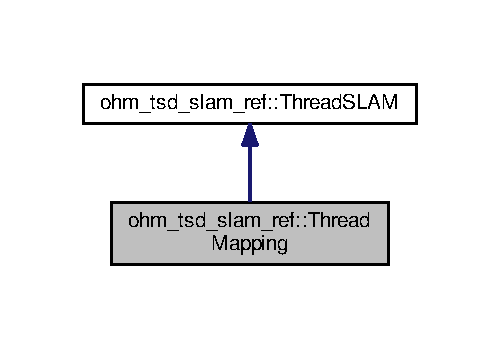
\includegraphics[width=240pt]{classohm__tsd__slam__ref_1_1ThreadMapping__inherit__graph}
\end{center}
\end{figure}


Collaboration diagram for ohm\-\_\-tsd\-\_\-slam\-\_\-ref\-:\-:Thread\-Mapping\-:\nopagebreak
\begin{figure}[H]
\begin{center}
\leavevmode
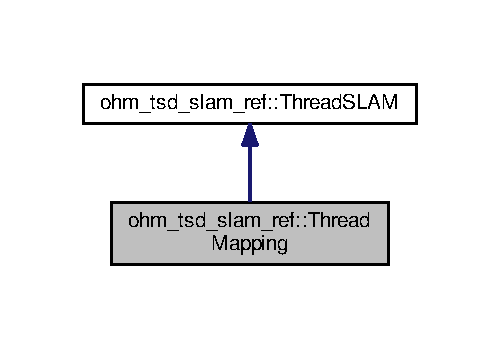
\includegraphics[width=240pt]{classohm__tsd__slam__ref_1_1ThreadMapping__coll__graph}
\end{center}
\end{figure}
\subsection*{Public Member Functions}
\begin{DoxyCompactItemize}
\item 
\hyperlink{classohm__tsd__slam__ref_1_1ThreadMapping_af5ba08d19538cdee50f17391084ba4c9}{Thread\-Mapping} (obvious\-::\-Tsd\-Grid $\ast$grid)
\item 
virtual \hyperlink{classohm__tsd__slam__ref_1_1ThreadMapping_afb1f328315a30d8066668af4f111ee40}{$\sim$\-Thread\-Mapping} ()
\item 
void \hyperlink{classohm__tsd__slam__ref_1_1ThreadMapping_aac36284866500920d4a23748be50aa2d}{queue\-Push} (obvious\-::\-Sensor\-Polar2\-D $\ast$sensor)
\item 
bool \hyperlink{classohm__tsd__slam__ref_1_1ThreadMapping_a28411f62f9383d0a533cee4cd270d81c}{initialized} (void)
\item 
void \hyperlink{classohm__tsd__slam__ref_1_1ThreadMapping_adb528149e6812dc8eba37ffe34801185}{init\-Push} (obvious\-::\-Sensor\-Polar2\-D $\ast$sensor)
\end{DoxyCompactItemize}
\subsection*{Protected Member Functions}
\begin{DoxyCompactItemize}
\item 
virtual void \hyperlink{classohm__tsd__slam__ref_1_1ThreadMapping_a4adf91a34a9cc1c237b180d02eb0b013}{event\-Loop} (void)
\end{DoxyCompactItemize}
\subsection*{Private Attributes}
\begin{DoxyCompactItemize}
\item 
std\-::deque\\*
$<$ obvious\-::\-Sensor\-Polar2\-D $\ast$ $>$ \hyperlink{classohm__tsd__slam__ref_1_1ThreadMapping_a789f75baff077164a69bb62b479c593d}{\-\_\-sensors}
\item 
boost\-::mutex \hyperlink{classohm__tsd__slam__ref_1_1ThreadMapping_a7c2899e1dd044dd21a98db7cf8b38a9d}{\-\_\-push\-Mutex}
\item 
bool \hyperlink{classohm__tsd__slam__ref_1_1ThreadMapping_a450952216cdda4e4a7b57d899429291c}{\-\_\-initialized}
\end{DoxyCompactItemize}
\subsection*{Additional Inherited Members}


\subsection{Detailed Description}
Implements a thread updating an obvious\-:Tsd\-Grid. 

\begin{DoxyAuthor}{Author}
Philipp Koch, Stefan May 
\end{DoxyAuthor}


\subsection{Constructor \& Destructor Documentation}
\hypertarget{classohm__tsd__slam__ref_1_1ThreadMapping_af5ba08d19538cdee50f17391084ba4c9}{\index{ohm\-\_\-tsd\-\_\-slam\-\_\-ref\-::\-Thread\-Mapping@{ohm\-\_\-tsd\-\_\-slam\-\_\-ref\-::\-Thread\-Mapping}!Thread\-Mapping@{Thread\-Mapping}}
\index{Thread\-Mapping@{Thread\-Mapping}!ohm_tsd_slam_ref::ThreadMapping@{ohm\-\_\-tsd\-\_\-slam\-\_\-ref\-::\-Thread\-Mapping}}
\subsubsection[{Thread\-Mapping}]{\setlength{\rightskip}{0pt plus 5cm}ohm\-\_\-tsd\-\_\-slam\-\_\-ref\-::\-Thread\-Mapping\-::\-Thread\-Mapping (
\begin{DoxyParamCaption}
\item[{obvious\-::\-Tsd\-Grid $\ast$}]{grid}
\end{DoxyParamCaption}
)}}\label{classohm__tsd__slam__ref_1_1ThreadMapping_af5ba08d19538cdee50f17391084ba4c9}
Constructor 
\begin{DoxyParams}{Parameters}
{\em grid} & Representation taken over from base class \hyperlink{classohm__tsd__slam__ref_1_1ThreadSLAM}{Thread\-S\-L\-A\-M} \\
\hline
\end{DoxyParams}
\hypertarget{classohm__tsd__slam__ref_1_1ThreadMapping_afb1f328315a30d8066668af4f111ee40}{\index{ohm\-\_\-tsd\-\_\-slam\-\_\-ref\-::\-Thread\-Mapping@{ohm\-\_\-tsd\-\_\-slam\-\_\-ref\-::\-Thread\-Mapping}!$\sim$\-Thread\-Mapping@{$\sim$\-Thread\-Mapping}}
\index{$\sim$\-Thread\-Mapping@{$\sim$\-Thread\-Mapping}!ohm_tsd_slam_ref::ThreadMapping@{ohm\-\_\-tsd\-\_\-slam\-\_\-ref\-::\-Thread\-Mapping}}
\subsubsection[{$\sim$\-Thread\-Mapping}]{\setlength{\rightskip}{0pt plus 5cm}ohm\-\_\-tsd\-\_\-slam\-\_\-ref\-::\-Thread\-Mapping\-::$\sim$\-Thread\-Mapping (
\begin{DoxyParamCaption}
{}
\end{DoxyParamCaption}
)\hspace{0.3cm}{\ttfamily [virtual]}}}\label{classohm__tsd__slam__ref_1_1ThreadMapping_afb1f328315a30d8066668af4f111ee40}
Desctructor 

\subsection{Member Function Documentation}
\hypertarget{classohm__tsd__slam__ref_1_1ThreadMapping_a4adf91a34a9cc1c237b180d02eb0b013}{\index{ohm\-\_\-tsd\-\_\-slam\-\_\-ref\-::\-Thread\-Mapping@{ohm\-\_\-tsd\-\_\-slam\-\_\-ref\-::\-Thread\-Mapping}!event\-Loop@{event\-Loop}}
\index{event\-Loop@{event\-Loop}!ohm_tsd_slam_ref::ThreadMapping@{ohm\-\_\-tsd\-\_\-slam\-\_\-ref\-::\-Thread\-Mapping}}
\subsubsection[{event\-Loop}]{\setlength{\rightskip}{0pt plus 5cm}void ohm\-\_\-tsd\-\_\-slam\-\_\-ref\-::\-Thread\-Mapping\-::event\-Loop (
\begin{DoxyParamCaption}
\item[{void}]{}
\end{DoxyParamCaption}
)\hspace{0.3cm}{\ttfamily [protected]}, {\ttfamily [virtual]}}}\label{classohm__tsd__slam__ref_1_1ThreadMapping_a4adf91a34a9cc1c237b180d02eb0b013}
abstract function derived from base class \hyperlink{classohm__tsd__slam__ref_1_1ThreadSLAM}{Thread\-S\-L\-A\-M}; consists of a loop the thread never leaves until a termination call occurs updates the representation with the first sensor element in the deque \-\_\-sensors and removes used sensor element; iterates until queue is empty -\/ enters blocked mode after that 

Implements \hyperlink{classohm__tsd__slam__ref_1_1ThreadSLAM_a7f8eec542ea75b833d981b9c4af5beb0}{ohm\-\_\-tsd\-\_\-slam\-\_\-ref\-::\-Thread\-S\-L\-A\-M}.

\hypertarget{classohm__tsd__slam__ref_1_1ThreadMapping_a28411f62f9383d0a533cee4cd270d81c}{\index{ohm\-\_\-tsd\-\_\-slam\-\_\-ref\-::\-Thread\-Mapping@{ohm\-\_\-tsd\-\_\-slam\-\_\-ref\-::\-Thread\-Mapping}!initialized@{initialized}}
\index{initialized@{initialized}!ohm_tsd_slam_ref::ThreadMapping@{ohm\-\_\-tsd\-\_\-slam\-\_\-ref\-::\-Thread\-Mapping}}
\subsubsection[{initialized}]{\setlength{\rightskip}{0pt plus 5cm}bool ohm\-\_\-tsd\-\_\-slam\-\_\-ref\-::\-Thread\-Mapping\-::initialized (
\begin{DoxyParamCaption}
\item[{void}]{}
\end{DoxyParamCaption}
)}}\label{classohm__tsd__slam__ref_1_1ThreadMapping_a28411f62f9383d0a533cee4cd270d81c}
Bool determining whether T\-S\-D grid contains data or not, called by \hyperlink{classohm__tsd__slam__ref_1_1ThreadLocalize}{Thread\-Localize} \begin{DoxyReturn}{Returns}
true in case of an initialized grid (contains data) 
\end{DoxyReturn}
\hypertarget{classohm__tsd__slam__ref_1_1ThreadMapping_adb528149e6812dc8eba37ffe34801185}{\index{ohm\-\_\-tsd\-\_\-slam\-\_\-ref\-::\-Thread\-Mapping@{ohm\-\_\-tsd\-\_\-slam\-\_\-ref\-::\-Thread\-Mapping}!init\-Push@{init\-Push}}
\index{init\-Push@{init\-Push}!ohm_tsd_slam_ref::ThreadMapping@{ohm\-\_\-tsd\-\_\-slam\-\_\-ref\-::\-Thread\-Mapping}}
\subsubsection[{init\-Push}]{\setlength{\rightskip}{0pt plus 5cm}void ohm\-\_\-tsd\-\_\-slam\-\_\-ref\-::\-Thread\-Mapping\-::init\-Push (
\begin{DoxyParamCaption}
\item[{obvious\-::\-Sensor\-Polar2\-D $\ast$}]{sensor}
\end{DoxyParamCaption}
)}}\label{classohm__tsd__slam__ref_1_1ThreadMapping_adb528149e6812dc8eba37ffe34801185}
Method to initialize the grid from a certain pose, called by \hyperlink{classohm__tsd__slam__ref_1_1ThreadLocalize}{Thread\-Localize} 
\begin{DoxyParams}{Parameters}
{\em sensor} & initial sensor data (pose, laser, mask..) \\
\hline
\end{DoxyParams}
\hypertarget{classohm__tsd__slam__ref_1_1ThreadMapping_aac36284866500920d4a23748be50aa2d}{\index{ohm\-\_\-tsd\-\_\-slam\-\_\-ref\-::\-Thread\-Mapping@{ohm\-\_\-tsd\-\_\-slam\-\_\-ref\-::\-Thread\-Mapping}!queue\-Push@{queue\-Push}}
\index{queue\-Push@{queue\-Push}!ohm_tsd_slam_ref::ThreadMapping@{ohm\-\_\-tsd\-\_\-slam\-\_\-ref\-::\-Thread\-Mapping}}
\subsubsection[{queue\-Push}]{\setlength{\rightskip}{0pt plus 5cm}void ohm\-\_\-tsd\-\_\-slam\-\_\-ref\-::\-Thread\-Mapping\-::queue\-Push (
\begin{DoxyParamCaption}
\item[{obvious\-::\-Sensor\-Polar2\-D $\ast$}]{sensor}
\end{DoxyParamCaption}
)}}\label{classohm__tsd__slam__ref_1_1ThreadMapping_aac36284866500920d4a23748be50aa2d}
Method to add an instance of Sensor\-Polar2\-D to the queue 
\begin{DoxyParams}{Parameters}
{\em sensor} & new sensor data (pose, laser, mask..) \\
\hline
\end{DoxyParams}


\subsection{Member Data Documentation}
\hypertarget{classohm__tsd__slam__ref_1_1ThreadMapping_a450952216cdda4e4a7b57d899429291c}{\index{ohm\-\_\-tsd\-\_\-slam\-\_\-ref\-::\-Thread\-Mapping@{ohm\-\_\-tsd\-\_\-slam\-\_\-ref\-::\-Thread\-Mapping}!\-\_\-initialized@{\-\_\-initialized}}
\index{\-\_\-initialized@{\-\_\-initialized}!ohm_tsd_slam_ref::ThreadMapping@{ohm\-\_\-tsd\-\_\-slam\-\_\-ref\-::\-Thread\-Mapping}}
\subsubsection[{\-\_\-initialized}]{\setlength{\rightskip}{0pt plus 5cm}bool ohm\-\_\-tsd\-\_\-slam\-\_\-ref\-::\-Thread\-Mapping\-::\-\_\-initialized\hspace{0.3cm}{\ttfamily [private]}}}\label{classohm__tsd__slam__ref_1_1ThreadMapping_a450952216cdda4e4a7b57d899429291c}
Flag initialized \hypertarget{classohm__tsd__slam__ref_1_1ThreadMapping_a7c2899e1dd044dd21a98db7cf8b38a9d}{\index{ohm\-\_\-tsd\-\_\-slam\-\_\-ref\-::\-Thread\-Mapping@{ohm\-\_\-tsd\-\_\-slam\-\_\-ref\-::\-Thread\-Mapping}!\-\_\-push\-Mutex@{\-\_\-push\-Mutex}}
\index{\-\_\-push\-Mutex@{\-\_\-push\-Mutex}!ohm_tsd_slam_ref::ThreadMapping@{ohm\-\_\-tsd\-\_\-slam\-\_\-ref\-::\-Thread\-Mapping}}
\subsubsection[{\-\_\-push\-Mutex}]{\setlength{\rightskip}{0pt plus 5cm}boost\-::mutex ohm\-\_\-tsd\-\_\-slam\-\_\-ref\-::\-Thread\-Mapping\-::\-\_\-push\-Mutex\hspace{0.3cm}{\ttfamily [private]}}}\label{classohm__tsd__slam__ref_1_1ThreadMapping_a7c2899e1dd044dd21a98db7cf8b38a9d}
Push mutex for double-\/ended-\/queue; synchronization necessary since queue is accessed by two threads method locks the mutex before adding data and unlocks it before terminating \hypertarget{classohm__tsd__slam__ref_1_1ThreadMapping_a789f75baff077164a69bb62b479c593d}{\index{ohm\-\_\-tsd\-\_\-slam\-\_\-ref\-::\-Thread\-Mapping@{ohm\-\_\-tsd\-\_\-slam\-\_\-ref\-::\-Thread\-Mapping}!\-\_\-sensors@{\-\_\-sensors}}
\index{\-\_\-sensors@{\-\_\-sensors}!ohm_tsd_slam_ref::ThreadMapping@{ohm\-\_\-tsd\-\_\-slam\-\_\-ref\-::\-Thread\-Mapping}}
\subsubsection[{\-\_\-sensors}]{\setlength{\rightskip}{0pt plus 5cm}std\-::deque$<$obvious\-::\-Sensor\-Polar2\-D$\ast$$>$ ohm\-\_\-tsd\-\_\-slam\-\_\-ref\-::\-Thread\-Mapping\-::\-\_\-sensors\hspace{0.3cm}{\ttfamily [private]}}}\label{classohm__tsd__slam__ref_1_1ThreadMapping_a789f75baff077164a69bb62b479c593d}
Sensor double-\/ended-\/queue, allows fast insertion and deletion at its beginning and end 

The documentation for this class was generated from the following files\-:\begin{DoxyCompactItemize}
\item 
src/\hyperlink{ThreadMapping_8h}{Thread\-Mapping.\-h}\item 
src/\hyperlink{ThreadMapping_8cpp}{Thread\-Mapping.\-cpp}\end{DoxyCompactItemize}

\hypertarget{classohm__tsd__slam__ref_1_1ThreadSLAM}{\section{ohm\-\_\-tsd\-\_\-slam\-\_\-ref\-:\-:Thread\-S\-L\-A\-M Class Reference}
\label{classohm__tsd__slam__ref_1_1ThreadSLAM}\index{ohm\-\_\-tsd\-\_\-slam\-\_\-ref\-::\-Thread\-S\-L\-A\-M@{ohm\-\_\-tsd\-\_\-slam\-\_\-ref\-::\-Thread\-S\-L\-A\-M}}
}


Base class implementing boost thread functionality.  




{\ttfamily \#include $<$Thread\-S\-L\-A\-M.\-h$>$}



Inheritance diagram for ohm\-\_\-tsd\-\_\-slam\-\_\-ref\-:\-:Thread\-S\-L\-A\-M\-:\nopagebreak
\begin{figure}[H]
\begin{center}
\leavevmode
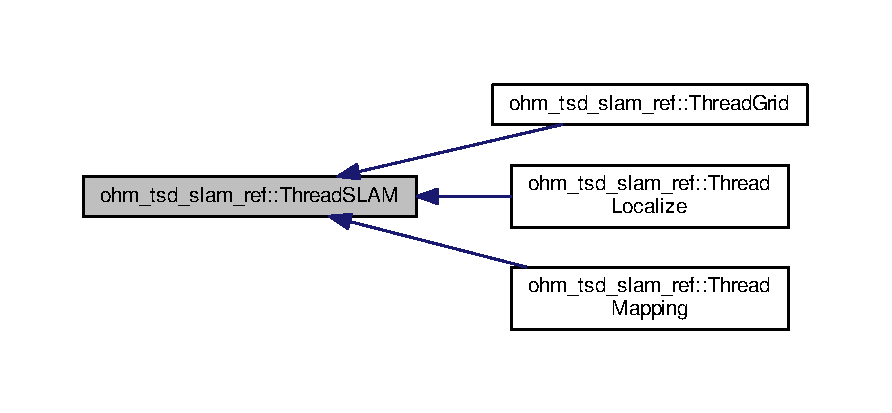
\includegraphics[width=350pt]{classohm__tsd__slam__ref_1_1ThreadSLAM__inherit__graph}
\end{center}
\end{figure}
\subsection*{Public Member Functions}
\begin{DoxyCompactItemize}
\item 
\hyperlink{classohm__tsd__slam__ref_1_1ThreadSLAM_ac2c871a0e2fcf8d5b0d8cd795d4c411c}{Thread\-S\-L\-A\-M} (obvious\-::\-Tsd\-Grid \&grid)
\item 
virtual \hyperlink{classohm__tsd__slam__ref_1_1ThreadSLAM_ac6855fff76f89863ef91186cd097cd87}{$\sim$\-Thread\-S\-L\-A\-M} ()
\item 
void \hyperlink{classohm__tsd__slam__ref_1_1ThreadSLAM_aa2516f5f4a5840bfc47c3314b5f62d48}{unblock} (void)
\item 
bool \hyperlink{classohm__tsd__slam__ref_1_1ThreadSLAM_adddd2cc23e446ffee1d2554f9d0f3a60}{alive} (unsigned int ms)
\item 
void \hyperlink{classohm__tsd__slam__ref_1_1ThreadSLAM_a3f3030728d97821ce6fb958587b93c83}{terminate\-Thread} (void)
\end{DoxyCompactItemize}
\subsection*{Protected Member Functions}
\begin{DoxyCompactItemize}
\item 
virtual void \hyperlink{classohm__tsd__slam__ref_1_1ThreadSLAM_a7f8eec542ea75b833d981b9c4af5beb0}{event\-Loop} (void)=0
\end{DoxyCompactItemize}
\subsection*{Protected Attributes}
\begin{DoxyCompactItemize}
\item 
boost\-::thread $\ast$ \hyperlink{classohm__tsd__slam__ref_1_1ThreadSLAM_af046376720757fbc1c2302809fd6ba07}{\-\_\-thread}
\item 
boost\-::mutex \hyperlink{classohm__tsd__slam__ref_1_1ThreadSLAM_aa461c69e9be71020e371babc6e534120}{\-\_\-sleep\-Mutex}
\item 
boost\-::condition\-\_\-variable\-\_\-any \hyperlink{classohm__tsd__slam__ref_1_1ThreadSLAM_a0302ee2027cf077f552395da5c618c30}{\-\_\-sleep\-Cond}
\item 
bool \hyperlink{classohm__tsd__slam__ref_1_1ThreadSLAM_a303f8c9d58dca22db1f1f9c0e37cf6e4}{\-\_\-stay\-Active}
\item 
obvious\-::\-Tsd\-Grid \& \hyperlink{classohm__tsd__slam__ref_1_1ThreadSLAM_ab0eaf26f3b9c549fe0d21332f88ccc35}{\-\_\-grid}
\end{DoxyCompactItemize}


\subsection{Detailed Description}
Base class implementing boost thread functionality. 

\begin{DoxyAuthor}{Author}
Philipp Koch, Stefan May 
\end{DoxyAuthor}


\subsection{Constructor \& Destructor Documentation}
\hypertarget{classohm__tsd__slam__ref_1_1ThreadSLAM_ac2c871a0e2fcf8d5b0d8cd795d4c411c}{\index{ohm\-\_\-tsd\-\_\-slam\-\_\-ref\-::\-Thread\-S\-L\-A\-M@{ohm\-\_\-tsd\-\_\-slam\-\_\-ref\-::\-Thread\-S\-L\-A\-M}!Thread\-S\-L\-A\-M@{Thread\-S\-L\-A\-M}}
\index{Thread\-S\-L\-A\-M@{Thread\-S\-L\-A\-M}!ohm_tsd_slam_ref::ThreadSLAM@{ohm\-\_\-tsd\-\_\-slam\-\_\-ref\-::\-Thread\-S\-L\-A\-M}}
\subsubsection[{Thread\-S\-L\-A\-M}]{\setlength{\rightskip}{0pt plus 5cm}ohm\-\_\-tsd\-\_\-slam\-\_\-ref\-::\-Thread\-S\-L\-A\-M\-::\-Thread\-S\-L\-A\-M (
\begin{DoxyParamCaption}
\item[{obvious\-::\-Tsd\-Grid \&}]{grid}
\end{DoxyParamCaption}
)}}\label{classohm__tsd__slam__ref_1_1ThreadSLAM_ac2c871a0e2fcf8d5b0d8cd795d4c411c}
Constructor \hypertarget{classohm__tsd__slam__ref_1_1ThreadSLAM_ac6855fff76f89863ef91186cd097cd87}{\index{ohm\-\_\-tsd\-\_\-slam\-\_\-ref\-::\-Thread\-S\-L\-A\-M@{ohm\-\_\-tsd\-\_\-slam\-\_\-ref\-::\-Thread\-S\-L\-A\-M}!$\sim$\-Thread\-S\-L\-A\-M@{$\sim$\-Thread\-S\-L\-A\-M}}
\index{$\sim$\-Thread\-S\-L\-A\-M@{$\sim$\-Thread\-S\-L\-A\-M}!ohm_tsd_slam_ref::ThreadSLAM@{ohm\-\_\-tsd\-\_\-slam\-\_\-ref\-::\-Thread\-S\-L\-A\-M}}
\subsubsection[{$\sim$\-Thread\-S\-L\-A\-M}]{\setlength{\rightskip}{0pt plus 5cm}ohm\-\_\-tsd\-\_\-slam\-\_\-ref\-::\-Thread\-S\-L\-A\-M\-::$\sim$\-Thread\-S\-L\-A\-M (
\begin{DoxyParamCaption}
{}
\end{DoxyParamCaption}
)\hspace{0.3cm}{\ttfamily [virtual]}}}\label{classohm__tsd__slam__ref_1_1ThreadSLAM_ac6855fff76f89863ef91186cd097cd87}
Destructor 

\subsection{Member Function Documentation}
\hypertarget{classohm__tsd__slam__ref_1_1ThreadSLAM_adddd2cc23e446ffee1d2554f9d0f3a60}{\index{ohm\-\_\-tsd\-\_\-slam\-\_\-ref\-::\-Thread\-S\-L\-A\-M@{ohm\-\_\-tsd\-\_\-slam\-\_\-ref\-::\-Thread\-S\-L\-A\-M}!alive@{alive}}
\index{alive@{alive}!ohm_tsd_slam_ref::ThreadSLAM@{ohm\-\_\-tsd\-\_\-slam\-\_\-ref\-::\-Thread\-S\-L\-A\-M}}
\subsubsection[{alive}]{\setlength{\rightskip}{0pt plus 5cm}bool ohm\-\_\-tsd\-\_\-slam\-\_\-ref\-::\-Thread\-S\-L\-A\-M\-::alive (
\begin{DoxyParamCaption}
\item[{unsigned int}]{ms}
\end{DoxyParamCaption}
)}}\label{classohm__tsd__slam__ref_1_1ThreadSLAM_adddd2cc23e446ffee1d2554f9d0f3a60}
Method to determine the state of a thread. Function tries to call the thread until the given time in ms runs out 
\begin{DoxyParams}{Parameters}
{\em ms} & time trying to call thread \\
\hline
\end{DoxyParams}
\begin{DoxyReturn}{Returns}
true if thread could be called successfully during given ms 
\end{DoxyReturn}
\hypertarget{classohm__tsd__slam__ref_1_1ThreadSLAM_a7f8eec542ea75b833d981b9c4af5beb0}{\index{ohm\-\_\-tsd\-\_\-slam\-\_\-ref\-::\-Thread\-S\-L\-A\-M@{ohm\-\_\-tsd\-\_\-slam\-\_\-ref\-::\-Thread\-S\-L\-A\-M}!event\-Loop@{event\-Loop}}
\index{event\-Loop@{event\-Loop}!ohm_tsd_slam_ref::ThreadSLAM@{ohm\-\_\-tsd\-\_\-slam\-\_\-ref\-::\-Thread\-S\-L\-A\-M}}
\subsubsection[{event\-Loop}]{\setlength{\rightskip}{0pt plus 5cm}virtual void ohm\-\_\-tsd\-\_\-slam\-\_\-ref\-::\-Thread\-S\-L\-A\-M\-::event\-Loop (
\begin{DoxyParamCaption}
\item[{void}]{}
\end{DoxyParamCaption}
)\hspace{0.3cm}{\ttfamily [protected]}, {\ttfamily [pure virtual]}}}\label{classohm__tsd__slam__ref_1_1ThreadSLAM_a7f8eec542ea75b833d981b9c4af5beb0}
Abstract method connected to Boost threading functionality 

Implemented in \hyperlink{classohm__tsd__slam__ref_1_1ThreadLocalize_a93b32600effe05fe0db9fdf74cd40aa7}{ohm\-\_\-tsd\-\_\-slam\-\_\-ref\-::\-Thread\-Localize}, \hyperlink{classohm__tsd__slam__ref_1_1ThreadMapping_a4adf91a34a9cc1c237b180d02eb0b013}{ohm\-\_\-tsd\-\_\-slam\-\_\-ref\-::\-Thread\-Mapping}, and \hyperlink{classohm__tsd__slam__ref_1_1ThreadGrid_ab5153ffea8c253924f5d5f1f05d9aa59}{ohm\-\_\-tsd\-\_\-slam\-\_\-ref\-::\-Thread\-Grid}.

\hypertarget{classohm__tsd__slam__ref_1_1ThreadSLAM_a3f3030728d97821ce6fb958587b93c83}{\index{ohm\-\_\-tsd\-\_\-slam\-\_\-ref\-::\-Thread\-S\-L\-A\-M@{ohm\-\_\-tsd\-\_\-slam\-\_\-ref\-::\-Thread\-S\-L\-A\-M}!terminate\-Thread@{terminate\-Thread}}
\index{terminate\-Thread@{terminate\-Thread}!ohm_tsd_slam_ref::ThreadSLAM@{ohm\-\_\-tsd\-\_\-slam\-\_\-ref\-::\-Thread\-S\-L\-A\-M}}
\subsubsection[{terminate\-Thread}]{\setlength{\rightskip}{0pt plus 5cm}void ohm\-\_\-tsd\-\_\-slam\-\_\-ref\-::\-Thread\-S\-L\-A\-M\-::terminate\-Thread (
\begin{DoxyParamCaption}
\item[{void}]{}
\end{DoxyParamCaption}
)}}\label{classohm__tsd__slam__ref_1_1ThreadSLAM_a3f3030728d97821ce6fb958587b93c83}
Method to terminate the thread \hypertarget{classohm__tsd__slam__ref_1_1ThreadSLAM_aa2516f5f4a5840bfc47c3314b5f62d48}{\index{ohm\-\_\-tsd\-\_\-slam\-\_\-ref\-::\-Thread\-S\-L\-A\-M@{ohm\-\_\-tsd\-\_\-slam\-\_\-ref\-::\-Thread\-S\-L\-A\-M}!unblock@{unblock}}
\index{unblock@{unblock}!ohm_tsd_slam_ref::ThreadSLAM@{ohm\-\_\-tsd\-\_\-slam\-\_\-ref\-::\-Thread\-S\-L\-A\-M}}
\subsubsection[{unblock}]{\setlength{\rightskip}{0pt plus 5cm}void ohm\-\_\-tsd\-\_\-slam\-\_\-ref\-::\-Thread\-S\-L\-A\-M\-::unblock (
\begin{DoxyParamCaption}
\item[{void}]{}
\end{DoxyParamCaption}
)}}\label{classohm__tsd__slam__ref_1_1ThreadSLAM_aa2516f5f4a5840bfc47c3314b5f62d48}
Method to set a thread from sleep mode to run mode 

\subsection{Member Data Documentation}
\hypertarget{classohm__tsd__slam__ref_1_1ThreadSLAM_ab0eaf26f3b9c549fe0d21332f88ccc35}{\index{ohm\-\_\-tsd\-\_\-slam\-\_\-ref\-::\-Thread\-S\-L\-A\-M@{ohm\-\_\-tsd\-\_\-slam\-\_\-ref\-::\-Thread\-S\-L\-A\-M}!\-\_\-grid@{\-\_\-grid}}
\index{\-\_\-grid@{\-\_\-grid}!ohm_tsd_slam_ref::ThreadSLAM@{ohm\-\_\-tsd\-\_\-slam\-\_\-ref\-::\-Thread\-S\-L\-A\-M}}
\subsubsection[{\-\_\-grid}]{\setlength{\rightskip}{0pt plus 5cm}obvious\-::\-Tsd\-Grid\& ohm\-\_\-tsd\-\_\-slam\-\_\-ref\-::\-Thread\-S\-L\-A\-M\-::\-\_\-grid\hspace{0.3cm}{\ttfamily [protected]}}}\label{classohm__tsd__slam__ref_1_1ThreadSLAM_ab0eaf26f3b9c549fe0d21332f88ccc35}
Reference to tsdgrid representation \hypertarget{classohm__tsd__slam__ref_1_1ThreadSLAM_a0302ee2027cf077f552395da5c618c30}{\index{ohm\-\_\-tsd\-\_\-slam\-\_\-ref\-::\-Thread\-S\-L\-A\-M@{ohm\-\_\-tsd\-\_\-slam\-\_\-ref\-::\-Thread\-S\-L\-A\-M}!\-\_\-sleep\-Cond@{\-\_\-sleep\-Cond}}
\index{\-\_\-sleep\-Cond@{\-\_\-sleep\-Cond}!ohm_tsd_slam_ref::ThreadSLAM@{ohm\-\_\-tsd\-\_\-slam\-\_\-ref\-::\-Thread\-S\-L\-A\-M}}
\subsubsection[{\-\_\-sleep\-Cond}]{\setlength{\rightskip}{0pt plus 5cm}boost\-::condition\-\_\-variable\-\_\-any ohm\-\_\-tsd\-\_\-slam\-\_\-ref\-::\-Thread\-S\-L\-A\-M\-::\-\_\-sleep\-Cond\hspace{0.3cm}{\ttfamily [protected]}}}\label{classohm__tsd__slam__ref_1_1ThreadSLAM_a0302ee2027cf077f552395da5c618c30}
Boost condition variable for sleeping mode \hypertarget{classohm__tsd__slam__ref_1_1ThreadSLAM_aa461c69e9be71020e371babc6e534120}{\index{ohm\-\_\-tsd\-\_\-slam\-\_\-ref\-::\-Thread\-S\-L\-A\-M@{ohm\-\_\-tsd\-\_\-slam\-\_\-ref\-::\-Thread\-S\-L\-A\-M}!\-\_\-sleep\-Mutex@{\-\_\-sleep\-Mutex}}
\index{\-\_\-sleep\-Mutex@{\-\_\-sleep\-Mutex}!ohm_tsd_slam_ref::ThreadSLAM@{ohm\-\_\-tsd\-\_\-slam\-\_\-ref\-::\-Thread\-S\-L\-A\-M}}
\subsubsection[{\-\_\-sleep\-Mutex}]{\setlength{\rightskip}{0pt plus 5cm}boost\-::mutex ohm\-\_\-tsd\-\_\-slam\-\_\-ref\-::\-Thread\-S\-L\-A\-M\-::\-\_\-sleep\-Mutex\hspace{0.3cm}{\ttfamily [protected]}}}\label{classohm__tsd__slam__ref_1_1ThreadSLAM_aa461c69e9be71020e371babc6e534120}
Boost sleeping mutex \hypertarget{classohm__tsd__slam__ref_1_1ThreadSLAM_a303f8c9d58dca22db1f1f9c0e37cf6e4}{\index{ohm\-\_\-tsd\-\_\-slam\-\_\-ref\-::\-Thread\-S\-L\-A\-M@{ohm\-\_\-tsd\-\_\-slam\-\_\-ref\-::\-Thread\-S\-L\-A\-M}!\-\_\-stay\-Active@{\-\_\-stay\-Active}}
\index{\-\_\-stay\-Active@{\-\_\-stay\-Active}!ohm_tsd_slam_ref::ThreadSLAM@{ohm\-\_\-tsd\-\_\-slam\-\_\-ref\-::\-Thread\-S\-L\-A\-M}}
\subsubsection[{\-\_\-stay\-Active}]{\setlength{\rightskip}{0pt plus 5cm}bool ohm\-\_\-tsd\-\_\-slam\-\_\-ref\-::\-Thread\-S\-L\-A\-M\-::\-\_\-stay\-Active\hspace{0.3cm}{\ttfamily [protected]}}}\label{classohm__tsd__slam__ref_1_1ThreadSLAM_a303f8c9d58dca22db1f1f9c0e37cf6e4}
Shutdown flag \hypertarget{classohm__tsd__slam__ref_1_1ThreadSLAM_af046376720757fbc1c2302809fd6ba07}{\index{ohm\-\_\-tsd\-\_\-slam\-\_\-ref\-::\-Thread\-S\-L\-A\-M@{ohm\-\_\-tsd\-\_\-slam\-\_\-ref\-::\-Thread\-S\-L\-A\-M}!\-\_\-thread@{\-\_\-thread}}
\index{\-\_\-thread@{\-\_\-thread}!ohm_tsd_slam_ref::ThreadSLAM@{ohm\-\_\-tsd\-\_\-slam\-\_\-ref\-::\-Thread\-S\-L\-A\-M}}
\subsubsection[{\-\_\-thread}]{\setlength{\rightskip}{0pt plus 5cm}boost\-::thread$\ast$ ohm\-\_\-tsd\-\_\-slam\-\_\-ref\-::\-Thread\-S\-L\-A\-M\-::\-\_\-thread\hspace{0.3cm}{\ttfamily [protected]}}}\label{classohm__tsd__slam__ref_1_1ThreadSLAM_af046376720757fbc1c2302809fd6ba07}
Boost threading object 

The documentation for this class was generated from the following files\-:\begin{DoxyCompactItemize}
\item 
src/\hyperlink{ThreadSLAM_8h}{Thread\-S\-L\-A\-M.\-h}\item 
src/\hyperlink{ThreadSLAM_8cpp}{Thread\-S\-L\-A\-M.\-cpp}\end{DoxyCompactItemize}

\chapter{File Documentation}
\hypertarget{slam__node_8cpp}{\section{src/slam\-\_\-node.cpp File Reference}
\label{slam__node_8cpp}\index{src/slam\-\_\-node.\-cpp@{src/slam\-\_\-node.\-cpp}}
}
{\ttfamily \#include \char`\"{}Slam\-Node.\-h\char`\"{}}\\*
{\ttfamily \#include $<$ros/ros.\-h$>$}\\*
{\ttfamily \#include \char`\"{}obcore/base/\-Logger.\-h\char`\"{}}\\*
Include dependency graph for slam\-\_\-node.\-cpp\-:\nopagebreak
\begin{figure}[H]
\begin{center}
\leavevmode
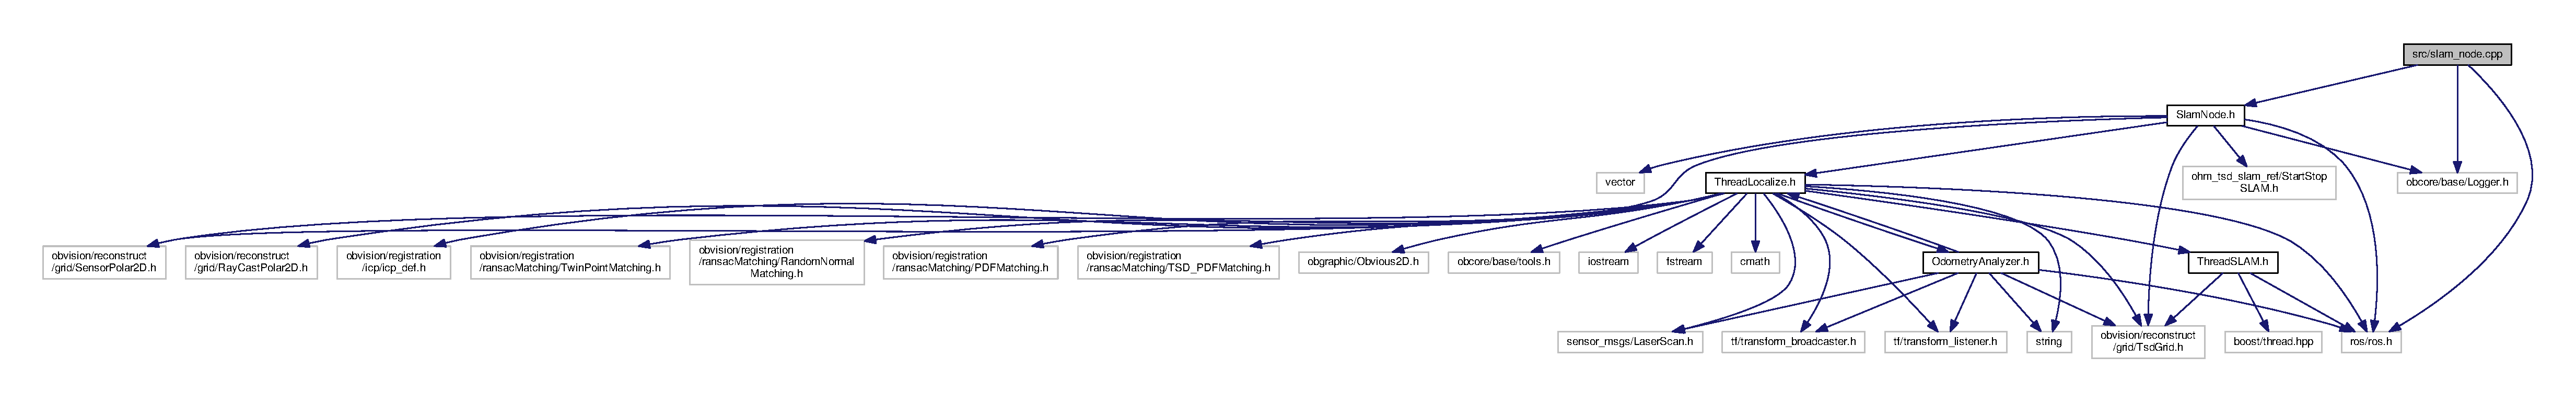
\includegraphics[width=350pt]{slam__node_8cpp__incl}
\end{center}
\end{figure}
\subsection*{Functions}
\begin{DoxyCompactItemize}
\item 
int \hyperlink{slam__node_8cpp_a3c04138a5bfe5d72780bb7e82a18e627}{main} (int argc, char $\ast$$\ast$argv)
\end{DoxyCompactItemize}


\subsection{Function Documentation}
\hypertarget{slam__node_8cpp_a3c04138a5bfe5d72780bb7e82a18e627}{\index{slam\-\_\-node.\-cpp@{slam\-\_\-node.\-cpp}!main@{main}}
\index{main@{main}!slam_node.cpp@{slam\-\_\-node.\-cpp}}
\subsubsection[{main}]{\setlength{\rightskip}{0pt plus 5cm}int main (
\begin{DoxyParamCaption}
\item[{int}]{argc, }
\item[{char $\ast$$\ast$}]{argv}
\end{DoxyParamCaption}
)}}\label{slam__node_8cpp_a3c04138a5bfe5d72780bb7e82a18e627}

\hypertarget{SlamNode_8cpp}{\section{src/\-Slam\-Node.cpp File Reference}
\label{SlamNode_8cpp}\index{src/\-Slam\-Node.\-cpp@{src/\-Slam\-Node.\-cpp}}
}
{\ttfamily \#include \char`\"{}Slam\-Node.\-h\char`\"{}}\\*
{\ttfamily \#include \char`\"{}Thread\-Mapping.\-h\char`\"{}}\\*
{\ttfamily \#include \char`\"{}Thread\-Grid.\-h\char`\"{}}\\*
{\ttfamily \#include \char`\"{}obcore/math/mathbase.\-h\char`\"{}}\\*
Include dependency graph for Slam\-Node.\-cpp\-:\nopagebreak
\begin{figure}[H]
\begin{center}
\leavevmode
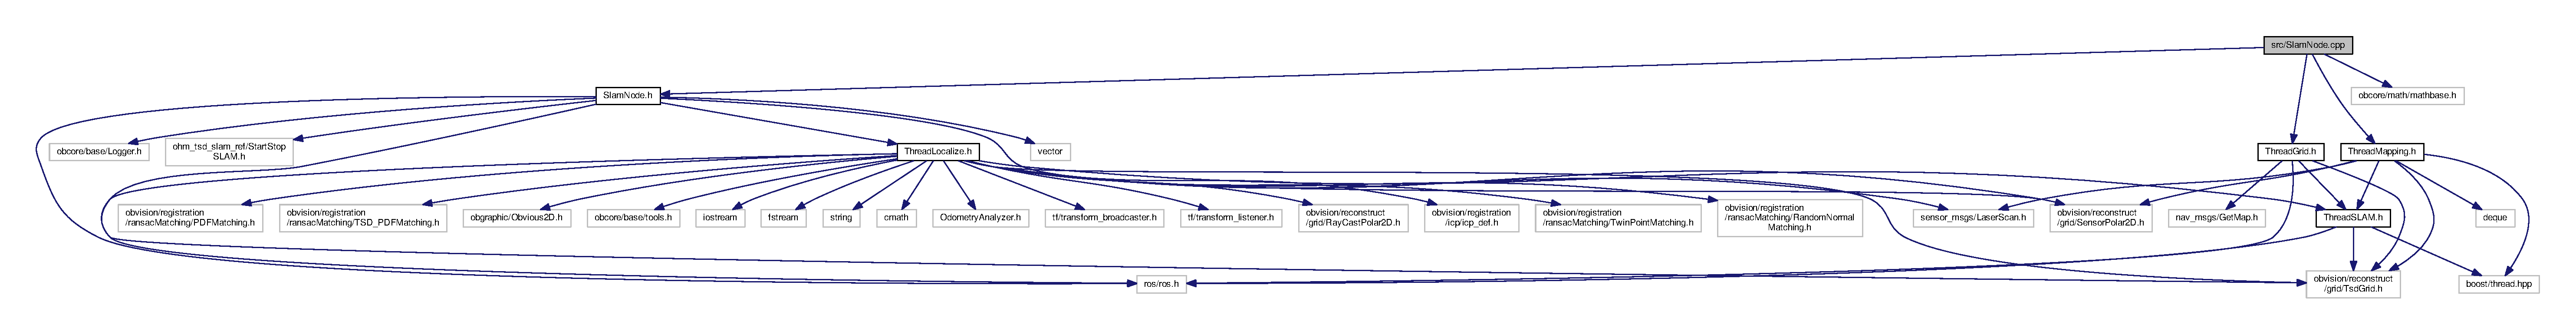
\includegraphics[width=350pt]{SlamNode_8cpp__incl}
\end{center}
\end{figure}
\subsection*{Namespaces}
\begin{DoxyCompactItemize}
\item 
\hyperlink{namespaceohm__tsd__slam__ref}{ohm\-\_\-tsd\-\_\-slam\-\_\-ref}
\begin{DoxyCompactList}\small\item\em todo whats T\-R\-A\-C\-E kommt unten nochmal \end{DoxyCompactList}\end{DoxyCompactItemize}

\hypertarget{SlamNode_8h}{\section{src/\-Slam\-Node.h File Reference}
\label{SlamNode_8h}\index{src/\-Slam\-Node.\-h@{src/\-Slam\-Node.\-h}}
}
{\ttfamily \#include $<$ros/ros.\-h$>$}\\*
{\ttfamily \#include $<$vector$>$}\\*
{\ttfamily \#include \char`\"{}obvision/reconstruct/grid/\-Tsd\-Grid.\-h\char`\"{}}\\*
{\ttfamily \#include \char`\"{}obvision/reconstruct/grid/\-Sensor\-Polar2\-D.\-h\char`\"{}}\\*
{\ttfamily \#include \char`\"{}obcore/base/\-Logger.\-h\char`\"{}}\\*
{\ttfamily \#include \char`\"{}Thread\-Localize.\-h\char`\"{}}\\*
{\ttfamily \#include \char`\"{}ohm\-\_\-tsd\-\_\-slam\-\_\-ref/\-Start\-Stop\-S\-L\-A\-M.\-h\char`\"{}}\\*
Include dependency graph for Slam\-Node.\-h\-:\nopagebreak
\begin{figure}[H]
\begin{center}
\leavevmode
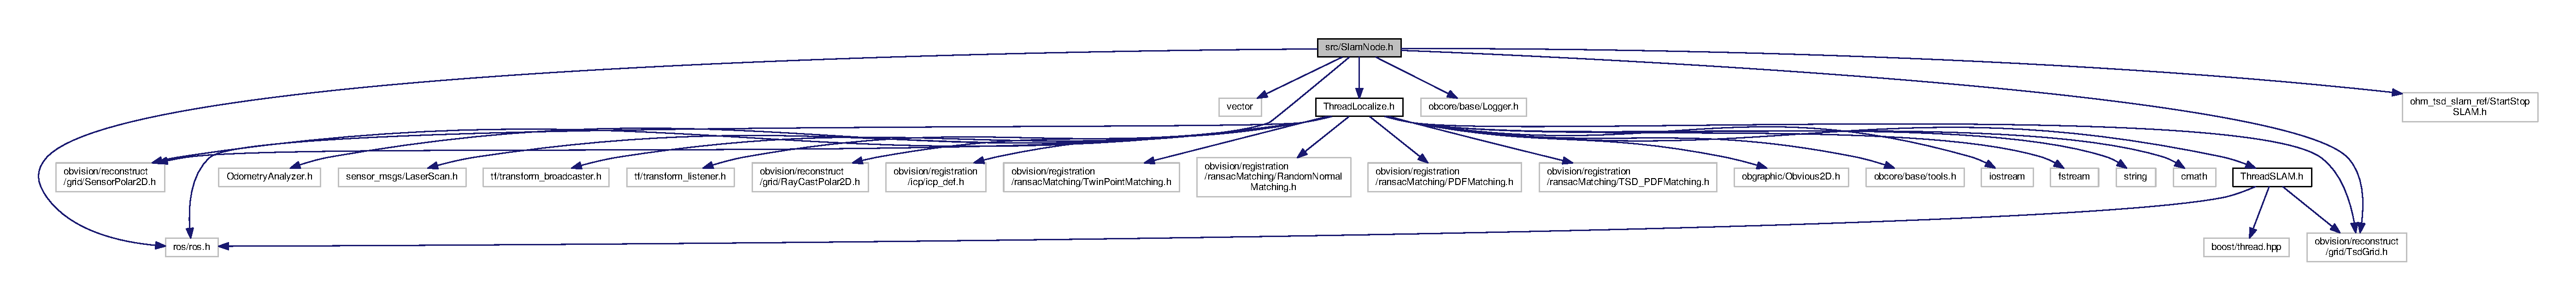
\includegraphics[width=350pt]{SlamNode_8h__incl}
\end{center}
\end{figure}
This graph shows which files directly or indirectly include this file\-:\nopagebreak
\begin{figure}[H]
\begin{center}
\leavevmode
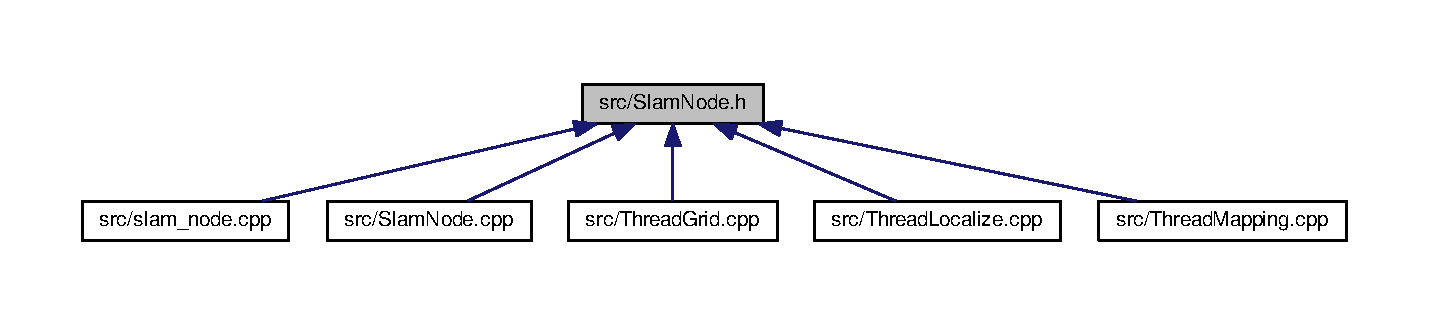
\includegraphics[width=350pt]{SlamNode_8h__dep__incl}
\end{center}
\end{figure}
\subsection*{Classes}
\begin{DoxyCompactItemize}
\item 
struct \hyperlink{structohm__tsd__slam__ref_1_1TaggedSubscriber}{ohm\-\_\-tsd\-\_\-slam\-\_\-ref\-::\-Tagged\-Subscriber}
\begin{DoxyCompactList}\small\item\em \hyperlink{structohm__tsd__slam__ref_1_1TaggedSubscriber}{Tagged\-Subscriber} struct creates new datatype of subscribers for ros communication. \end{DoxyCompactList}\item 
class \hyperlink{classohm__tsd__slam__ref_1_1SlamNode}{ohm\-\_\-tsd\-\_\-slam\-\_\-ref\-::\-Slam\-Node}
\begin{DoxyCompactList}\small\item\em main node management of 2\-D slam, contains sub classes and ros interface \end{DoxyCompactList}\end{DoxyCompactItemize}
\subsection*{Namespaces}
\begin{DoxyCompactItemize}
\item 
\hyperlink{namespaceohm__tsd__slam__ref}{ohm\-\_\-tsd\-\_\-slam\-\_\-ref}
\end{DoxyCompactItemize}
\subsection*{Macros}
\begin{DoxyCompactItemize}
\item 
\#define \hyperlink{SlamNode_8h_a7f516bedc9360ce81c38b2b6fbd1a5ff}{I\-N\-I\-T\-\_\-\-P\-S\-H\-S}~1
\begin{DoxyCompactList}\small\item\em I\-N\-I\-T\-\_\-\-P\-S\-H\-S number of initial pushes into the grid. \end{DoxyCompactList}\item 
\#define \hyperlink{SlamNode_8h_a502d892a0b86363c94e2f11fb2370346}{T\-H\-R\-E\-A\-D\-\_\-\-T\-E\-R\-M\-\_\-\-M\-S}~1
\begin{DoxyCompactList}\small\item\em T\-H\-R\-E\-A\-D\-\_\-\-T\-E\-R\-M\-\_\-\-M\-S amount of time (ms) waiting for thread to terminate. \end{DoxyCompactList}\end{DoxyCompactItemize}


\subsection{Macro Definition Documentation}
\hypertarget{SlamNode_8h_a7f516bedc9360ce81c38b2b6fbd1a5ff}{\index{Slam\-Node.\-h@{Slam\-Node.\-h}!I\-N\-I\-T\-\_\-\-P\-S\-H\-S@{I\-N\-I\-T\-\_\-\-P\-S\-H\-S}}
\index{I\-N\-I\-T\-\_\-\-P\-S\-H\-S@{I\-N\-I\-T\-\_\-\-P\-S\-H\-S}!SlamNode.h@{Slam\-Node.\-h}}
\subsubsection[{I\-N\-I\-T\-\_\-\-P\-S\-H\-S}]{\setlength{\rightskip}{0pt plus 5cm}\#define I\-N\-I\-T\-\_\-\-P\-S\-H\-S~1}}\label{SlamNode_8h_a7f516bedc9360ce81c38b2b6fbd1a5ff}


I\-N\-I\-T\-\_\-\-P\-S\-H\-S number of initial pushes into the grid. 

\hypertarget{SlamNode_8h_a502d892a0b86363c94e2f11fb2370346}{\index{Slam\-Node.\-h@{Slam\-Node.\-h}!T\-H\-R\-E\-A\-D\-\_\-\-T\-E\-R\-M\-\_\-\-M\-S@{T\-H\-R\-E\-A\-D\-\_\-\-T\-E\-R\-M\-\_\-\-M\-S}}
\index{T\-H\-R\-E\-A\-D\-\_\-\-T\-E\-R\-M\-\_\-\-M\-S@{T\-H\-R\-E\-A\-D\-\_\-\-T\-E\-R\-M\-\_\-\-M\-S}!SlamNode.h@{Slam\-Node.\-h}}
\subsubsection[{T\-H\-R\-E\-A\-D\-\_\-\-T\-E\-R\-M\-\_\-\-M\-S}]{\setlength{\rightskip}{0pt plus 5cm}\#define T\-H\-R\-E\-A\-D\-\_\-\-T\-E\-R\-M\-\_\-\-M\-S~1}}\label{SlamNode_8h_a502d892a0b86363c94e2f11fb2370346}


T\-H\-R\-E\-A\-D\-\_\-\-T\-E\-R\-M\-\_\-\-M\-S amount of time (ms) waiting for thread to terminate. 

\begin{DoxyRefDesc}{Todo}
\item[\hyperlink{todo__todo000006}{Todo}]in Thread\-Grid wird im Destruktor thread\-::join() aus boost aufgerufen, um auf Beendigung des Threads zu warten. Slam\-Node erbt aber nicht von Thread\-S\-L\-A\-M, also besitzt es auch kein boost object thread. wäre es denkbar das auch damit zu lösen anstatt diese Zeit hier festzusetzen? \end{DoxyRefDesc}

\hypertarget{ThreadGrid_8cpp}{\section{src/\-Thread\-Grid.cpp File Reference}
\label{ThreadGrid_8cpp}\index{src/\-Thread\-Grid.\-cpp@{src/\-Thread\-Grid.\-cpp}}
}
{\ttfamily \#include \char`\"{}Thread\-Grid.\-h\char`\"{}}\\*
{\ttfamily \#include \char`\"{}Slam\-Node.\-h\char`\"{}}\\*
{\ttfamily \#include $<$string$>$}\\*
{\ttfamily \#include \char`\"{}obvision/reconstruct/grid/\-Ray\-Cast\-Axis\-Aligned2\-D.\-h\char`\"{}}\\*
{\ttfamily \#include \char`\"{}obcore/base/\-Logger.\-h\char`\"{}}\\*
{\ttfamily \#include $<$sensor\-\_\-msgs/\-Image.\-h$>$}\\*
{\ttfamily \#include $<$sensor\-\_\-msgs/image\-\_\-encodings.\-h$>$}\\*
Include dependency graph for Thread\-Grid.\-cpp\-:\nopagebreak
\begin{figure}[H]
\begin{center}
\leavevmode
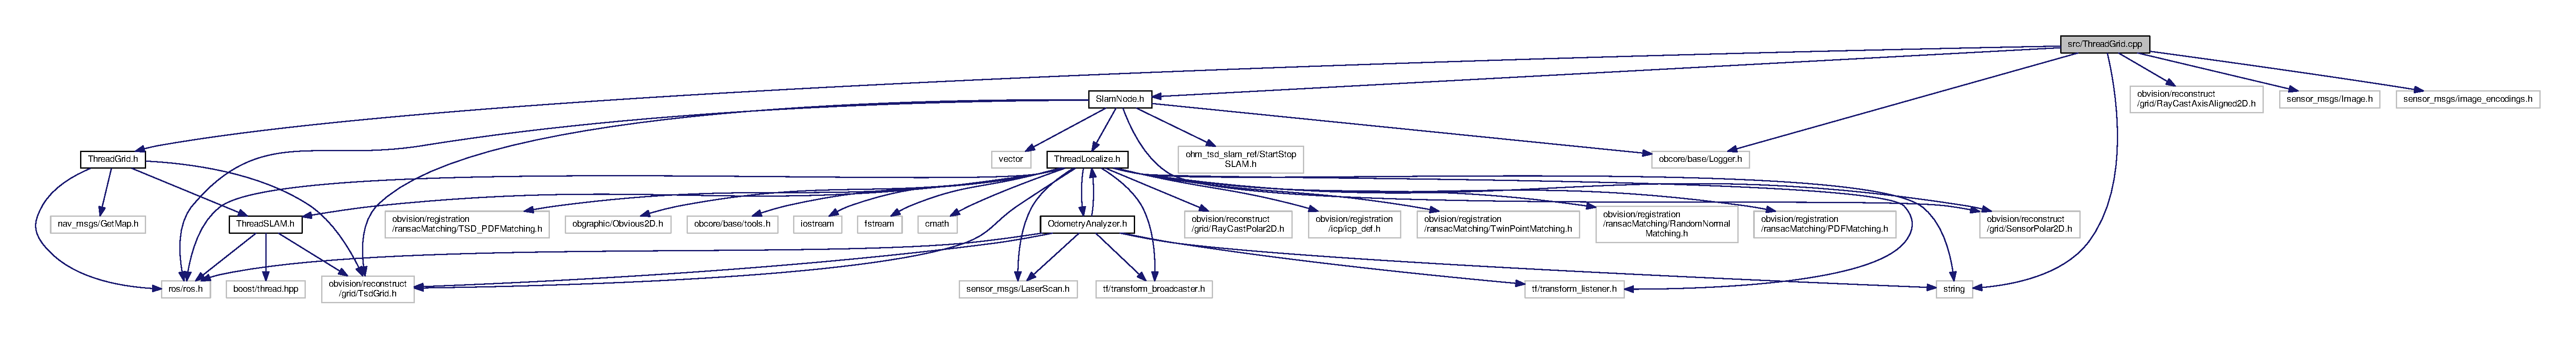
\includegraphics[width=350pt]{ThreadGrid_8cpp__incl}
\end{center}
\end{figure}
\subsection*{Namespaces}
\begin{DoxyCompactItemize}
\item 
\hyperlink{namespaceohm__tsd__slam__ref}{ohm\-\_\-tsd\-\_\-slam\-\_\-ref}
\end{DoxyCompactItemize}

\hypertarget{ThreadGrid_8h}{\section{src/\-Thread\-Grid.h File Reference}
\label{ThreadGrid_8h}\index{src/\-Thread\-Grid.\-h@{src/\-Thread\-Grid.\-h}}
}
{\ttfamily \#include \char`\"{}Thread\-S\-L\-A\-M.\-h\char`\"{}}\\*
{\ttfamily \#include \char`\"{}obvision/reconstruct/grid/\-Tsd\-Grid.\-h\char`\"{}}\\*
{\ttfamily \#include $<$ros/ros.\-h$>$}\\*
{\ttfamily \#include $<$nav\-\_\-msgs/\-Get\-Map.\-h$>$}\\*
Include dependency graph for Thread\-Grid.\-h\-:\nopagebreak
\begin{figure}[H]
\begin{center}
\leavevmode
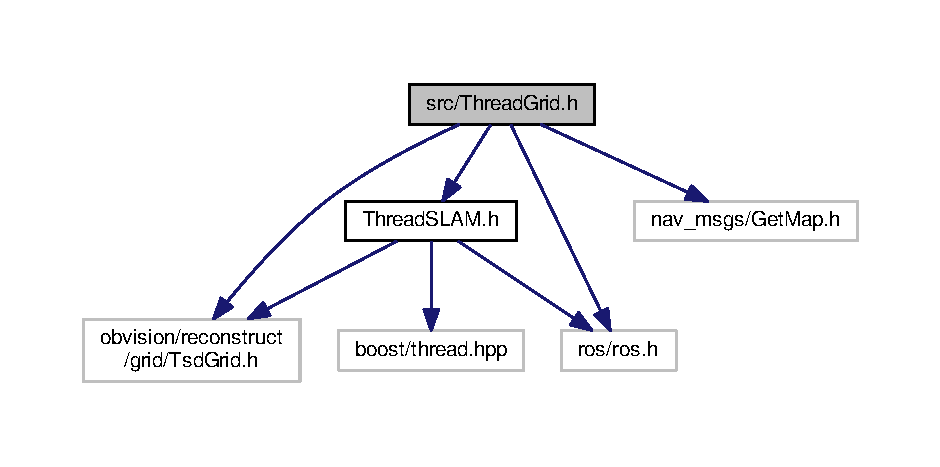
\includegraphics[width=350pt]{ThreadGrid_8h__incl}
\end{center}
\end{figure}
This graph shows which files directly or indirectly include this file\-:\nopagebreak
\begin{figure}[H]
\begin{center}
\leavevmode
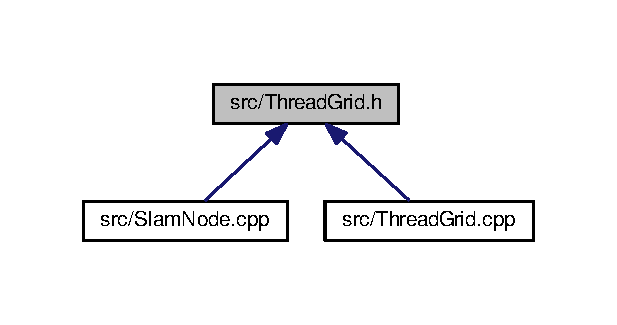
\includegraphics[width=296pt]{ThreadGrid_8h__dep__incl}
\end{center}
\end{figure}
\subsection*{Classes}
\begin{DoxyCompactItemize}
\item 
class \hyperlink{classohm__tsd__slam__ref_1_1ThreadGrid}{ohm\-\_\-tsd\-\_\-slam\-\_\-ref\-::\-Thread\-Grid}
\begin{DoxyCompactList}\small\item\em Class implementing a thread that generates an occupancy grid. \end{DoxyCompactList}\end{DoxyCompactItemize}
\subsection*{Namespaces}
\begin{DoxyCompactItemize}
\item 
\hyperlink{namespaceohm__tsd__slam__ref}{ohm\-\_\-tsd\-\_\-slam\-\_\-ref}
\begin{DoxyCompactList}\small\item\em todo whats T\-R\-A\-C\-E kommt unten nochmal \end{DoxyCompactList}\end{DoxyCompactItemize}

\hypertarget{ThreadLocalize_8cpp}{\section{src/\-Thread\-Localize.cpp File Reference}
\label{ThreadLocalize_8cpp}\index{src/\-Thread\-Localize.\-cpp@{src/\-Thread\-Localize.\-cpp}}
}
{\ttfamily \#include \char`\"{}Thread\-Localize.\-h\char`\"{}}\\*
{\ttfamily \#include \char`\"{}Slam\-Node.\-h\char`\"{}}\\*
{\ttfamily \#include \char`\"{}Thread\-Mapping.\-h\char`\"{}}\\*
{\ttfamily \#include \char`\"{}obcore/math/linalg/linalg.\-h\char`\"{}}\\*
{\ttfamily \#include \char`\"{}obcore/base/\-Logger.\-h\char`\"{}}\\*
{\ttfamily \#include $<$boost/bind.\-hpp$>$}\\*
{\ttfamily \#include $<$cstring$>$}\\*
{\ttfamily \#include $<$unistd.\-h$>$}\\*
{\ttfamily \#include $<$geometry\-\_\-msgs/\-Pose\-Stamped.\-h$>$}\\*
{\ttfamily \#include $<$tf/tf.\-h$>$}\\*
Include dependency graph for Thread\-Localize.\-cpp\-:\nopagebreak
\begin{figure}[H]
\begin{center}
\leavevmode
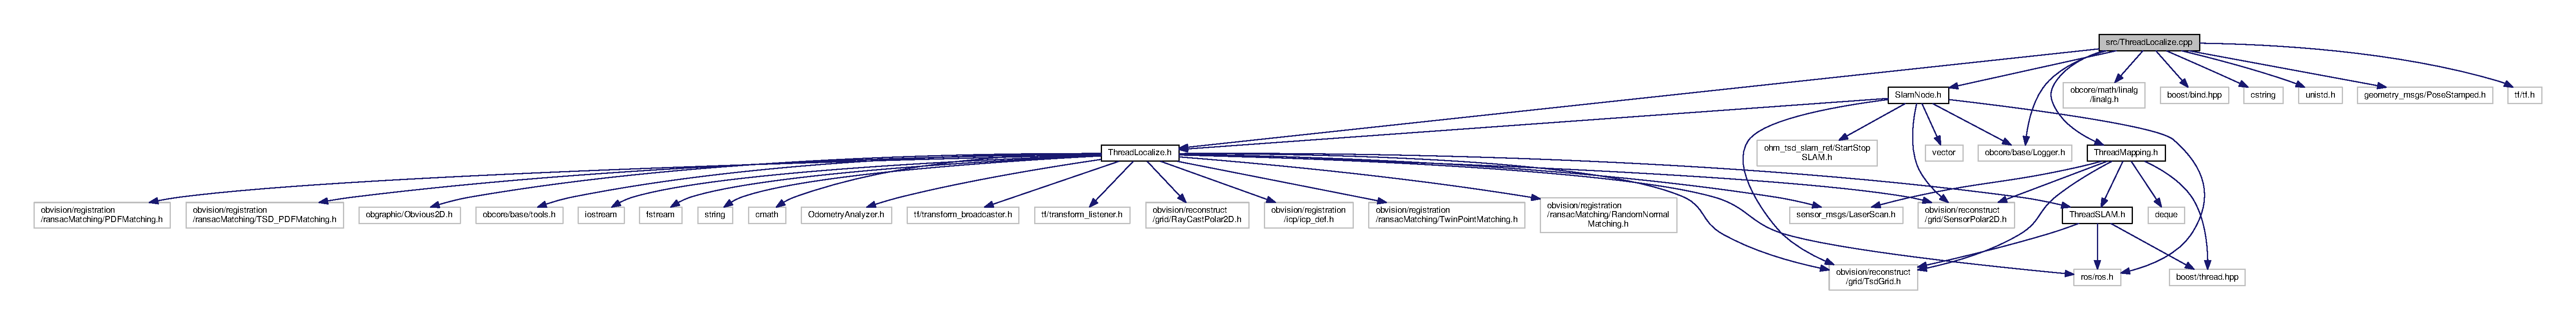
\includegraphics[width=350pt]{ThreadLocalize_8cpp__incl}
\end{center}
\end{figure}

\hypertarget{ThreadLocalize_8h}{\section{src/\-Thread\-Localize.h File Reference}
\label{ThreadLocalize_8h}\index{src/\-Thread\-Localize.\-h@{src/\-Thread\-Localize.\-h}}
}
{\ttfamily \#include \char`\"{}Thread\-S\-L\-A\-M.\-h\char`\"{}}\\*
{\ttfamily \#include \char`\"{}Odometry\-Analyzer.\-h\char`\"{}}\\*
{\ttfamily \#include $<$sensor\-\_\-msgs/\-Laser\-Scan.\-h$>$}\\*
{\ttfamily \#include $<$ros/ros.\-h$>$}\\*
{\ttfamily \#include $<$tf/transform\-\_\-broadcaster.\-h$>$}\\*
{\ttfamily \#include $<$tf/transform\-\_\-listener.\-h$>$}\\*
{\ttfamily \#include \char`\"{}obvision/reconstruct/grid/\-Sensor\-Polar2\-D.\-h\char`\"{}}\\*
{\ttfamily \#include \char`\"{}obvision/reconstruct/grid/\-Tsd\-Grid.\-h\char`\"{}}\\*
{\ttfamily \#include \char`\"{}obvision/reconstruct/grid/\-Ray\-Cast\-Polar2\-D.\-h\char`\"{}}\\*
{\ttfamily \#include \char`\"{}obvision/registration/icp/icp\-\_\-def.\-h\char`\"{}}\\*
{\ttfamily \#include \char`\"{}obvision/registration/ransac\-Matching/\-Twin\-Point\-Matching.\-h\char`\"{}}\\*
{\ttfamily \#include \char`\"{}obvision/registration/ransac\-Matching/\-Random\-Normal\-Matching.\-h\char`\"{}}\\*
{\ttfamily \#include \char`\"{}obvision/registration/ransac\-Matching/\-P\-D\-F\-Matching.\-h\char`\"{}}\\*
{\ttfamily \#include \char`\"{}obvision/registration/ransac\-Matching/\-T\-S\-D\-\_\-\-P\-D\-F\-Matching.\-h\char`\"{}}\\*
{\ttfamily \#include \char`\"{}obgraphic/\-Obvious2\-D.\-h\char`\"{}}\\*
{\ttfamily \#include \char`\"{}obcore/base/tools.\-h\char`\"{}}\\*
{\ttfamily \#include $<$iostream$>$}\\*
{\ttfamily \#include $<$fstream$>$}\\*
{\ttfamily \#include $<$string$>$}\\*
{\ttfamily \#include $<$cmath$>$}\\*
Include dependency graph for Thread\-Localize.\-h\-:\nopagebreak
\begin{figure}[H]
\begin{center}
\leavevmode
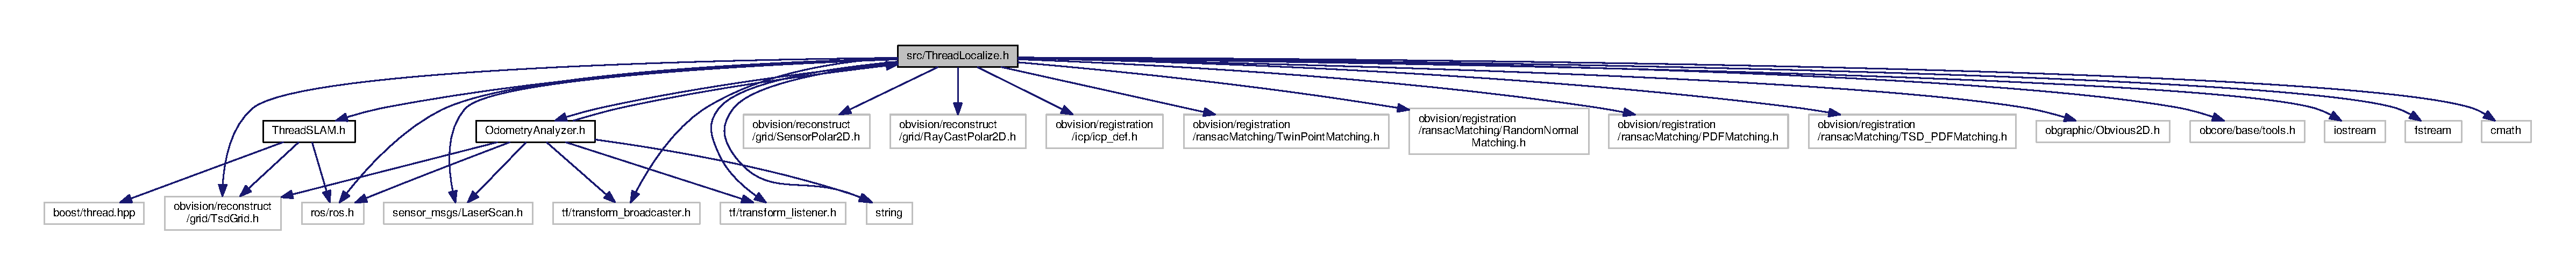
\includegraphics[width=350pt]{ThreadLocalize_8h__incl}
\end{center}
\end{figure}
This graph shows which files directly or indirectly include this file\-:\nopagebreak
\begin{figure}[H]
\begin{center}
\leavevmode
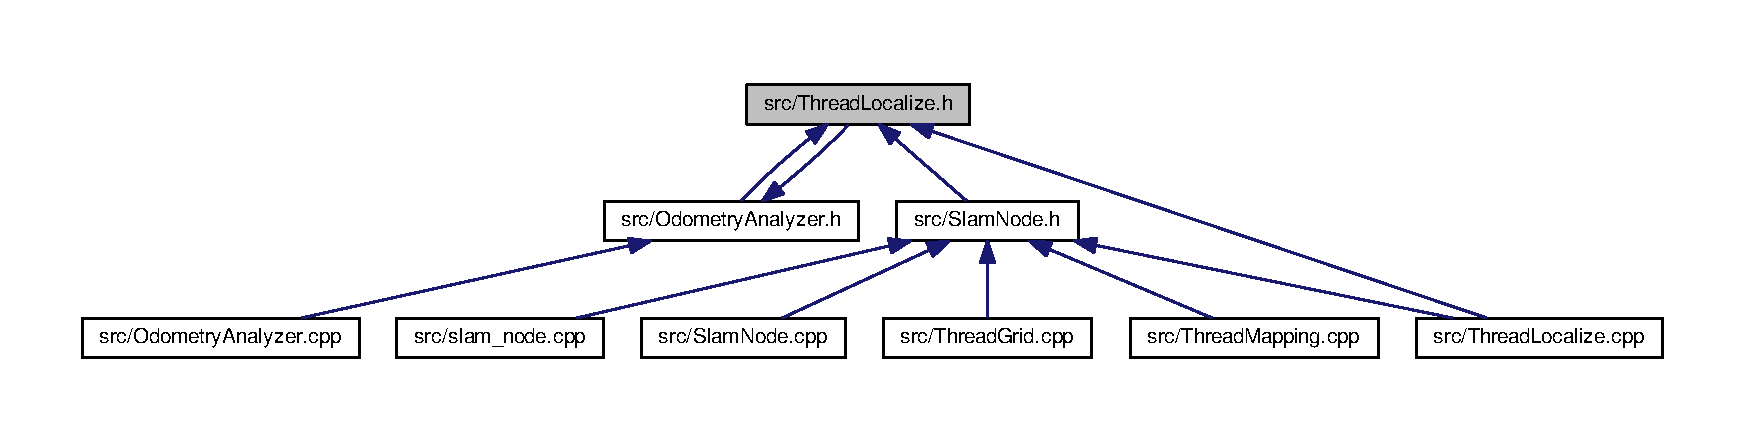
\includegraphics[width=350pt]{ThreadLocalize_8h__dep__incl}
\end{center}
\end{figure}
\subsection*{Classes}
\begin{DoxyCompactItemize}
\item 
class \hyperlink{classohm__tsd__slam__ref_1_1ThreadLocalize}{ohm\-\_\-tsd\-\_\-slam\-\_\-ref\-::\-Thread\-Localize}
\end{DoxyCompactItemize}
\subsection*{Namespaces}
\begin{DoxyCompactItemize}
\item 
\hyperlink{namespaceohm__tsd__slam__ref}{ohm\-\_\-tsd\-\_\-slam\-\_\-ref}
\begin{DoxyCompactList}\small\item\em todo whats T\-R\-A\-C\-E kommt unten nochmal \end{DoxyCompactList}\end{DoxyCompactItemize}

\hypertarget{ThreadMapping_8cpp}{\section{src/\-Thread\-Mapping.cpp File Reference}
\label{ThreadMapping_8cpp}\index{src/\-Thread\-Mapping.\-cpp@{src/\-Thread\-Mapping.\-cpp}}
}
{\ttfamily \#include \char`\"{}Thread\-Mapping.\-h\char`\"{}}\\*
{\ttfamily \#include \char`\"{}Slam\-Node.\-h\char`\"{}}\\*
{\ttfamily \#include \char`\"{}obcore/base/\-Logger.\-h\char`\"{}}\\*
{\ttfamily \#include \char`\"{}obcore/math/mathbase.\-h\char`\"{}}\\*
{\ttfamily \#include $<$cmath$>$}\\*
Include dependency graph for Thread\-Mapping.\-cpp\-:\nopagebreak
\begin{figure}[H]
\begin{center}
\leavevmode
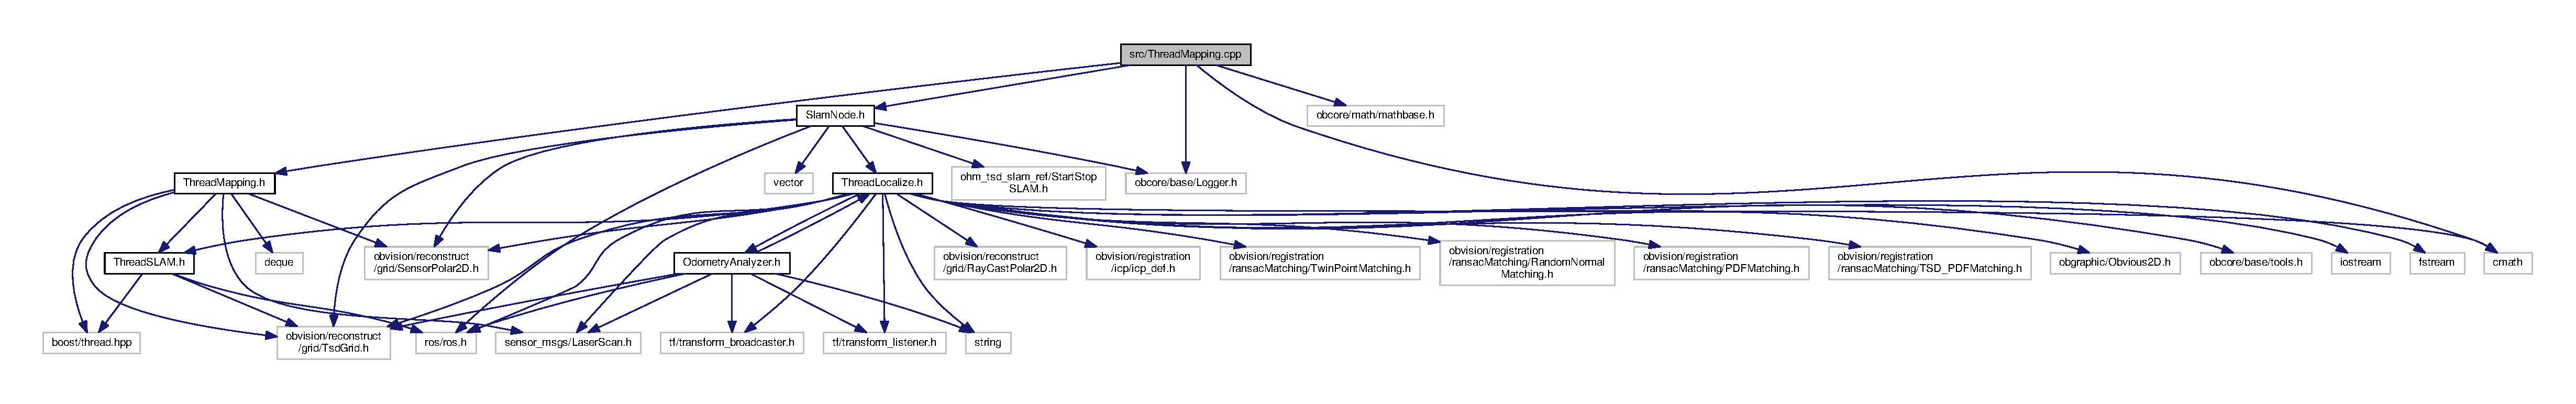
\includegraphics[width=350pt]{ThreadMapping_8cpp__incl}
\end{center}
\end{figure}
\subsection*{Namespaces}
\begin{DoxyCompactItemize}
\item 
\hyperlink{namespaceohm__tsd__slam__ref}{ohm\-\_\-tsd\-\_\-slam\-\_\-ref}
\end{DoxyCompactItemize}

\hypertarget{ThreadMapping_8h}{\section{src/\-Thread\-Mapping.h File Reference}
\label{ThreadMapping_8h}\index{src/\-Thread\-Mapping.\-h@{src/\-Thread\-Mapping.\-h}}
}
{\ttfamily \#include \char`\"{}Thread\-S\-L\-A\-M.\-h\char`\"{}}\\*
{\ttfamily \#include \char`\"{}sensor\-\_\-msgs/\-Laser\-Scan.\-h\char`\"{}}\\*
{\ttfamily \#include \char`\"{}obvision/reconstruct/grid/\-Sensor\-Polar2\-D.\-h\char`\"{}}\\*
{\ttfamily \#include \char`\"{}obvision/reconstruct/grid/\-Tsd\-Grid.\-h\char`\"{}}\\*
{\ttfamily \#include $<$boost/thread.\-hpp$>$}\\*
{\ttfamily \#include $<$deque$>$}\\*
Include dependency graph for Thread\-Mapping.\-h\-:\nopagebreak
\begin{figure}[H]
\begin{center}
\leavevmode
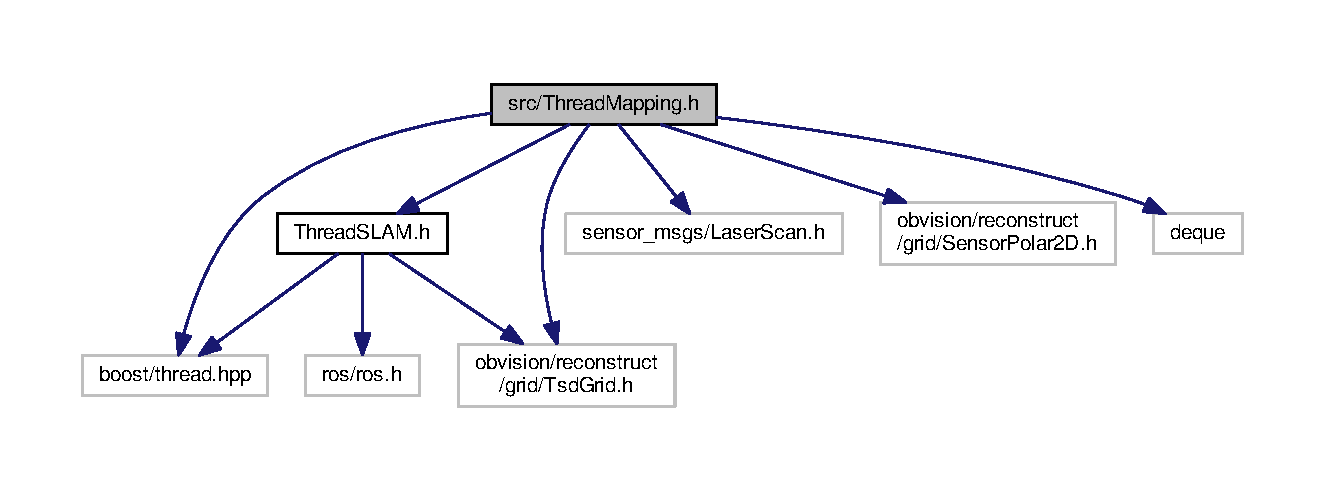
\includegraphics[width=350pt]{ThreadMapping_8h__incl}
\end{center}
\end{figure}
This graph shows which files directly or indirectly include this file\-:\nopagebreak
\begin{figure}[H]
\begin{center}
\leavevmode
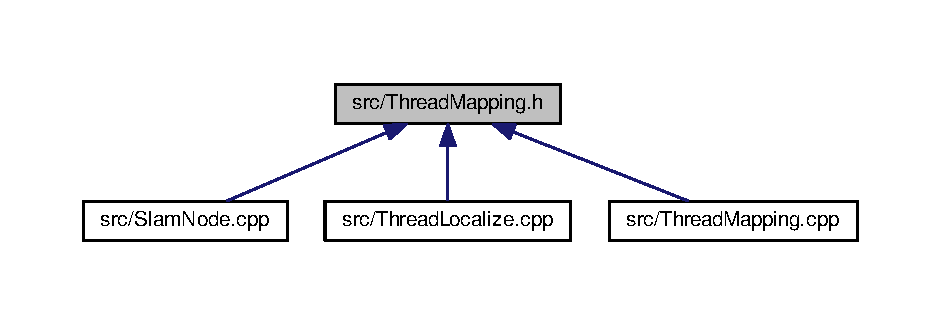
\includegraphics[width=350pt]{ThreadMapping_8h__dep__incl}
\end{center}
\end{figure}
\subsection*{Classes}
\begin{DoxyCompactItemize}
\item 
class \hyperlink{classohm__tsd__slam__ref_1_1ThreadMapping}{ohm\-\_\-tsd\-\_\-slam\-\_\-ref\-::\-Thread\-Mapping}
\begin{DoxyCompactList}\small\item\em Implements a thread updating an obvious\-:Tsd\-Grid. \end{DoxyCompactList}\end{DoxyCompactItemize}
\subsection*{Namespaces}
\begin{DoxyCompactItemize}
\item 
\hyperlink{namespaceohm__tsd__slam__ref}{ohm\-\_\-tsd\-\_\-slam\-\_\-ref}
\end{DoxyCompactItemize}

\hypertarget{ThreadSLAM_8cpp}{\section{src/\-Thread\-S\-L\-A\-M.cpp File Reference}
\label{ThreadSLAM_8cpp}\index{src/\-Thread\-S\-L\-A\-M.\-cpp@{src/\-Thread\-S\-L\-A\-M.\-cpp}}
}
{\ttfamily \#include \char`\"{}Thread\-S\-L\-A\-M.\-h\char`\"{}}\\*
Include dependency graph for Thread\-S\-L\-A\-M.\-cpp\-:\nopagebreak
\begin{figure}[H]
\begin{center}
\leavevmode
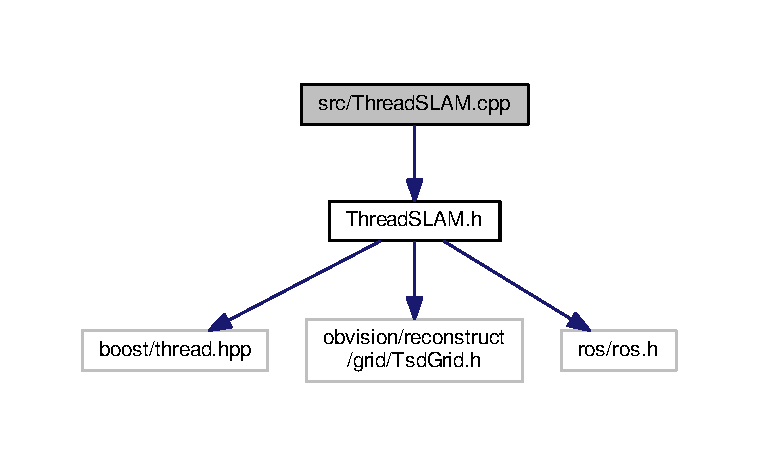
\includegraphics[width=350pt]{ThreadSLAM_8cpp__incl}
\end{center}
\end{figure}
\subsection*{Namespaces}
\begin{DoxyCompactItemize}
\item 
\hyperlink{namespaceohm__tsd__slam__ref}{ohm\-\_\-tsd\-\_\-slam\-\_\-ref}
\begin{DoxyCompactList}\small\item\em todo whats T\-R\-A\-C\-E kommt unten nochmal \end{DoxyCompactList}\end{DoxyCompactItemize}

\hypertarget{ThreadSLAM_8h}{\section{src/\-Thread\-S\-L\-A\-M.h File Reference}
\label{ThreadSLAM_8h}\index{src/\-Thread\-S\-L\-A\-M.\-h@{src/\-Thread\-S\-L\-A\-M.\-h}}
}
{\ttfamily \#include $<$boost/thread.\-hpp$>$}\\*
{\ttfamily \#include \char`\"{}obvision/reconstruct/grid/\-Tsd\-Grid.\-h\char`\"{}}\\*
{\ttfamily \#include $<$ros/ros.\-h$>$}\\*
Include dependency graph for Thread\-S\-L\-A\-M.\-h\-:\nopagebreak
\begin{figure}[H]
\begin{center}
\leavevmode
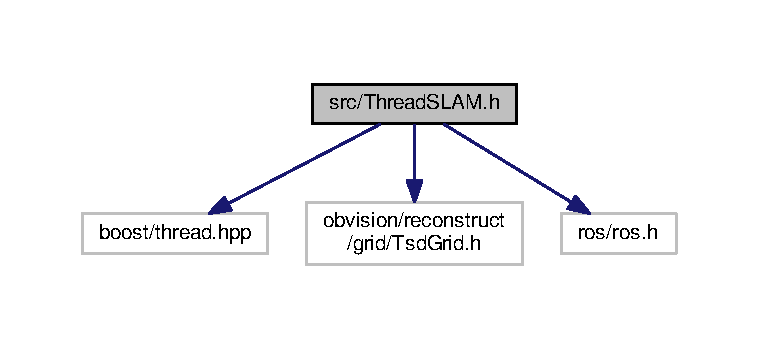
\includegraphics[width=350pt]{ThreadSLAM_8h__incl}
\end{center}
\end{figure}
This graph shows which files directly or indirectly include this file\-:\nopagebreak
\begin{figure}[H]
\begin{center}
\leavevmode
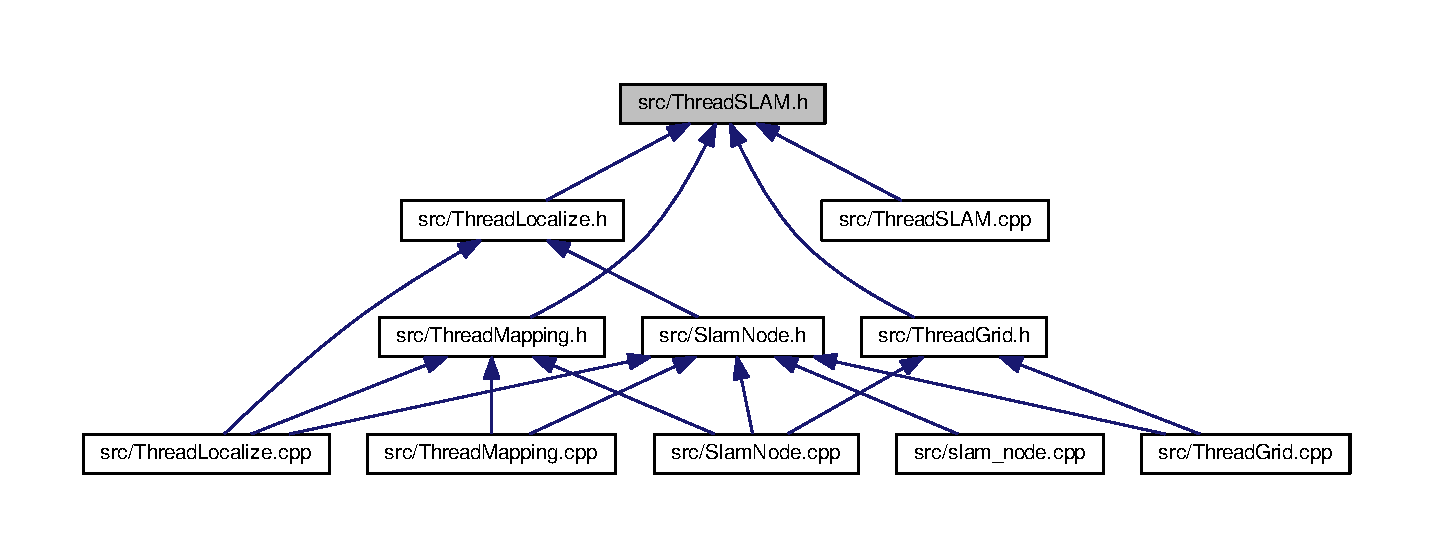
\includegraphics[width=350pt]{ThreadSLAM_8h__dep__incl}
\end{center}
\end{figure}
\subsection*{Classes}
\begin{DoxyCompactItemize}
\item 
class \hyperlink{classohm__tsd__slam__ref_1_1ThreadSLAM}{ohm\-\_\-tsd\-\_\-slam\-\_\-ref\-::\-Thread\-S\-L\-A\-M}
\begin{DoxyCompactList}\small\item\em Base class implementing boost thread functionality. \end{DoxyCompactList}\end{DoxyCompactItemize}
\subsection*{Namespaces}
\begin{DoxyCompactItemize}
\item 
\hyperlink{namespaceohm__tsd__slam__ref}{ohm\-\_\-tsd\-\_\-slam\-\_\-ref}
\end{DoxyCompactItemize}

%--- End generated contents ---

% Index
\newpage
\phantomsection
\addcontentsline{toc}{chapter}{Index}
\printindex

\end{document}
